\documentclass{../../../yukibook.cls/yukibook}

\makeatletter
\@addtoreset{chapter}{part}

\begin{document}

\yukibook{Sistemas Operativos \linebreak en red} 	% Title
  {Rubén Gómez}  % Author
  {2021-2022}    % Year
  {Técnico en Sistemas microinformáticos y redes} % Name of degree
  {}	% catch phrase
  {}	% the phrase's author
  {img/cover.png}

%--------------------------------------------------------------------------
% Start your parts, chapters and sections here
%--------------------------------------------------------------------------
\part{Windows Server 2019 como servidor de red}
\graphicspath{{img/windows/}}
\chapter{Un poco de historia}

Windows Server es la línea de productos de Microsoft \textbf{enfocada a servidores} que se inició con la primera versión: Windows 2000.

Anteriormente, Microsoft contaba con una línea también dedicada a estaciones de trabajo y servidores en red cuyo nombre era Windows NT, por lo que se puede considerar que \textbf{Windows Server es la continuación de NT} con el cambio de nombre.

Las versiones más importantes han sido, sin contar las denominadas NT:
\begin{itemize}
    \item Windows 2000.
    \item Windows Server 2003.
    \item Windows Server 2008.
    \item Windows Server 2012.
    \item Windows Server 2016.
    \item Windows Server 2019.
\end{itemize}

\chapter{Proceso de instalación de Windows Server 2019}
Para realizar la instalación de Windows Server 2019 necesitaremos el medio desde el que realizaremos la instalación. Microsoft permite la descarga desde su página oficial una evaluación de 180 días que podremos descargar en varios formatos:

\begin{itemize}
    \item \textbf{Azure}: Es el sistema “en la nube” de Microsoft. Se puede probar Windows Server a través de una cuenta gratuita y posteriormente gestionar los sistemas virtualizados que se creen en la nube.
    \item \textbf{ISO}: Una imagen ISO que podremos utilizar grabándolo en un DVD, a través de un USB o usarlo en un sistema de virtualización propio.
    \item \textbf{VHD}: Formato de archivo que representa una unidad de disco duro virtual.
\end{itemize}

Para realizar una instalación completa en nuestro sistema de virtualización elegiremos el archivo ISO. Para poder descargarlo tendremos que rellenar un formulario, elegir el idioma y posteriormente comenzará la descarga.

\section{Requisitos previos}
Antes de realizar la instalación debemos conocer cuáles son los requisitos mínimos de hardware que necesita Windows Server para así asegurar que la máquina virtual (o el hardware donde lo vamos a instalar) es 100\% compatible. En este caso, y tal como nos indica la web de Microsoft, los requisitos son:

\begin{itemize}
    \item \textbf{Procesador} de 64 bits a 1,4 GHz, compatible con el conjunto de instrucciones x64
    \begin{itemize}
        \item Admite DEP y NX
        \item Admite CMPXCHG16b, LAHF/SAHF y PrefetchW
        \item Admite la traducción de direcciones de segundo nivel (EPT o NPT)
    \end{itemize}
    \item \textbf{RAM}: 512 MB (\textbf{2 GB} para la opción de instalación Servidor con Experiencia de escritorio). Se admite RAM tipo ECC (código de corrección de errores)
    \item \textbf{Espacio en disco}:  mínimo 32GB. Windows Server no admite discos ATA, PATA, IDE y EIDE para unidades de arranque, página o datos.
    \item \textbf{Adaptador de red} de 1 gigabit/s
\end{itemize}

Dado que estos son los requisitos mínimos, nuestra máquina virtual deberá cumplirlos, pero en un sistema que vaya a estar en producción deberemos realizar un análisis de requisitos para asegurar que el hardware (ya sea virtual o físico) cumple las necesidades de los servicios que alojará:

\begin{itemize}
    \item ¿El servidor va a contar con un servidor web?
    \begin{itemize}
        \item ¿Cuántas visitas se esperan?
        \item ¿Qué tipo de web va a servir? ¿Programada en Java, PHP, …?
    \end{itemize}
    \item ¿El servidor va a contar con un sistema gestor de base de datos?
    \begin{itemize}
        \item ¿Cuántas bases de datos va a tener?
        \item ¿Cuántas conexiones simultáneas esperamos?
        \item ¿Cuántas peticiones estimamos que va a recibir?
    \end{itemize}
    \item ¿El servidor va a servir para compartir ficheros?
    \begin{itemize}
        \item ¿Cuántos usuarios van a acceder?
        \item ¿Peticiones estimadas?
    \end{itemize}
    \item …
\end{itemize}

Por tanto, antes de realizar la instalación, deberemos confirmar que conocemos para qué se va a utilizar el servidor, cuántos servicios se van a utilizar y la carga esperada.

\section{Instalación de Windows Server 2019}
El asistente de instalación de Windows Server nos va a llevar por una serie de pasos que detallaremos a continuación.
\warnbox{Nos aseguramos que la máquina virtual arranque desde la ISO}

\subsection{Elección del idioma}

El primer paso del asistente será elegir el idioma principal que usaremos en el sistema operativo.
Antes de realizar la descarga de la ISO hemos elegido el idioma español, por lo que el asistente nos aparecerá por defecto en ese idioma. Podremos elegir:

{
    \begin{minipage}{0.6\linewidth}
        \setlength{\parskip}{1.2em}
        \begin{itemize}
            \item Idioma que va a instalar
            \item Formato de hora y moneda
            \item Teclado o método de entrada
        \end{itemize}

        En nuestro caso dejaremos las opciones tal como nos aparece por defecto, pero de utilizar el servidor en un sistema internacional, convendría hacer uso del sistema en inglés.
    \end{minipage}
    \hfill
    \begin{minipage}{0.36\linewidth}
            \vspace{-11pt}
            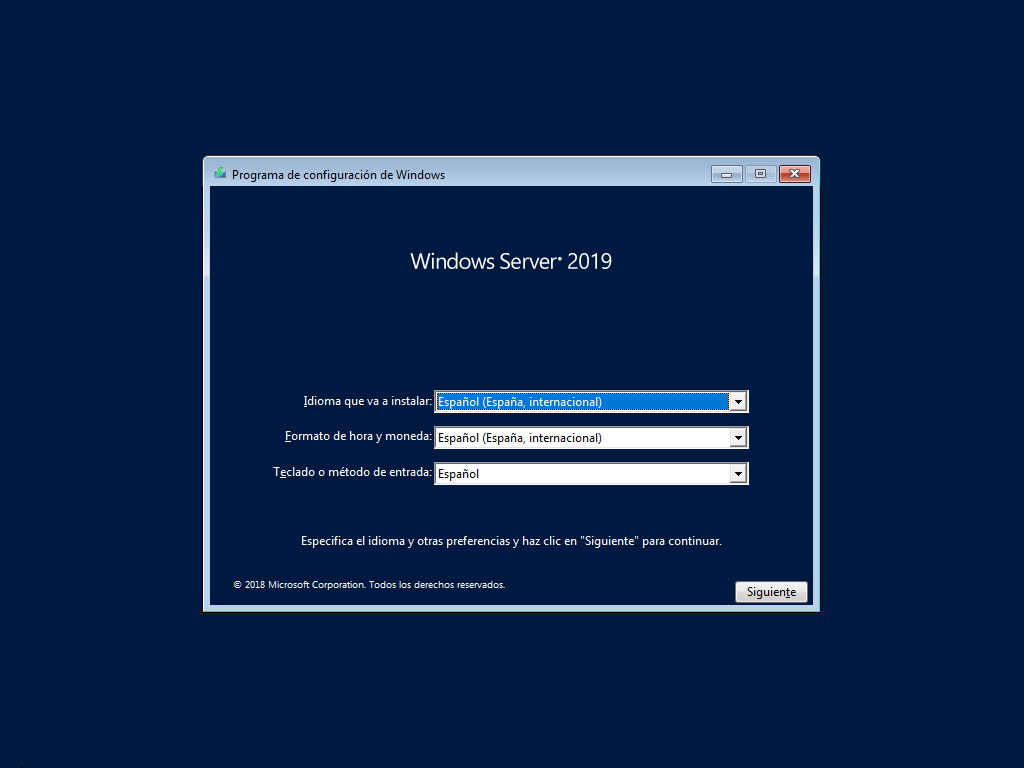
\includegraphics[trim={202 155 203 155},clip,width=\linewidth]{1_instalacion.png}
    \end{minipage}
}

\subsection{Elección del sistema operativo}
Windows Server 2019 tiene distintos modos a la hora de ser instalado, tal como podemos ver en la siguiente captura de pantalla del proceso de instalación:
\begin{center}
    \vspace{-10pt}
    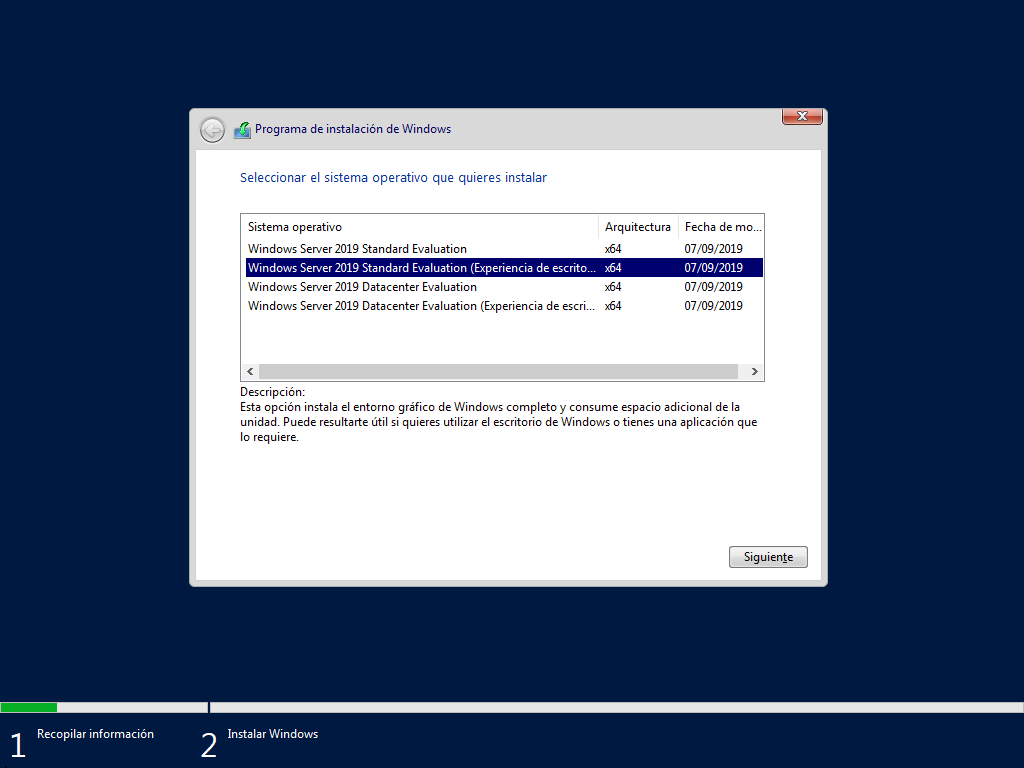
\includegraphics[trim={188 180 195 107},clip,width=10cm]{2_instalacion.png}
    \vspace{-15pt}
\end{center}

Existen dos opciones principales a la hora de elegir, ya que cada una de ellas permitirá instalarlo con o sin experiencia de escritorio. Las opciones principales son:

\begin{itemize}
    \item \textbf{Standard Evaluation}: Útil para empresas medianas o pequeñas, que no requieran de grandes sistemas de virtualización.
    \item \textbf{Datacenter Evaluation}: No habrá límite a la hora de crear máquinas virtuales con un host Hyper-V por cada licencia.
\end{itemize}

Existen más diferencias, y es por eso que Microsoft tiene una página dedicada con la \href{https://docs.microsoft.com/es-es/windows-server/get-started/editions-comparison-windows-server-2019}{comparación de ambas versiones}. Por lo tanto, antes de realizar la instalación para nuestro sistema, debemos realizar una estimación de los requisitos para así poder elegir de manera adecuada.

Nosotros vamos a elegir la versión “Standard Evaluation” con experiencia de escritorio ya que podremos realizar la configuración desde el propio servidor. Dependiendo del caso, habrá que analizar cuál es la mejor opción antes de realizar la instalación.

Al darle a “Siguiente” nos aparecerán los términos de la licencia.

\subsection{Tipo de instalación}
Tras aceptar la licencia nos aparecerá el tipo de instalación que deseamos realizar:
\begin{center}
    \vspace{-10pt}
    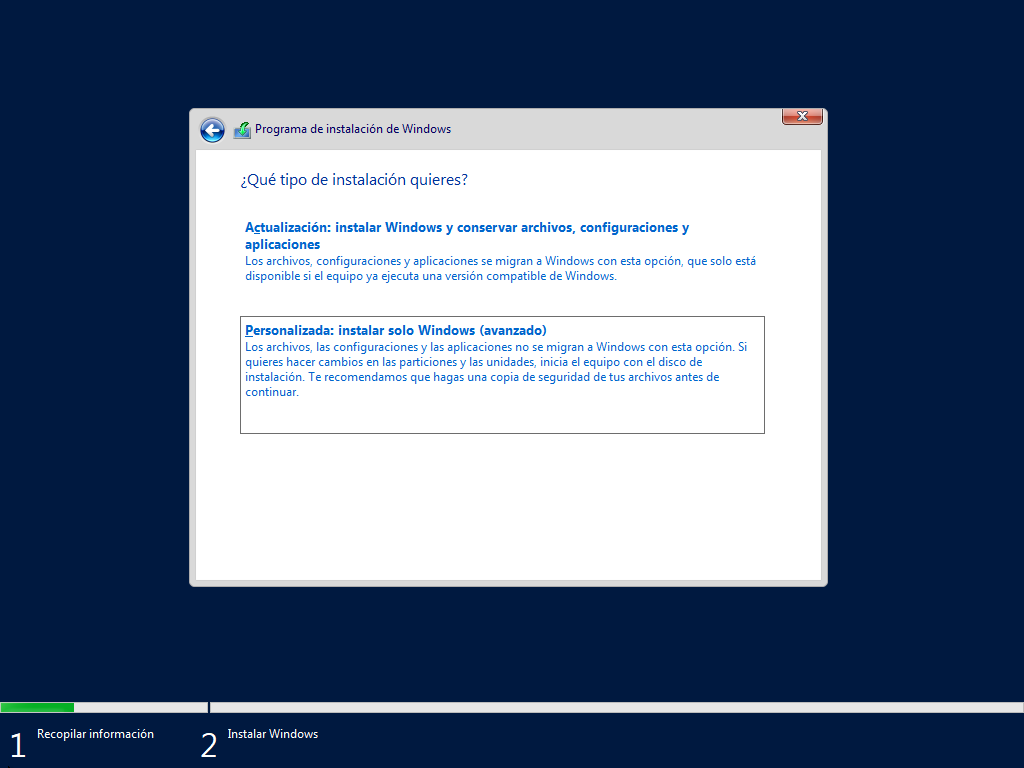
\includegraphics[trim={188 180 195 107},clip,width=10cm]{3_instalacion.png}
    \vspace{-10pt}
\end{center}

\begin{itemize}
    \item \textbf{Actualización}: Para realizar actualizaciones sobre sistemas compatibles ya instalados.
    \item \textbf{Personalizada}: Tal como indica la imagen anterior, los archivos, las configuraciones y las aplicaciones no se migran. En caso de realizar una instalación nueva (como en nuestro caso), \textbf{utilizaremos esta opción}.
\end{itemize}

\subsection{Particionado de discos duros}
Dado que nuestra máquina virtual es nueva, y no tiene ningún sistema operativo previo, vamos a tener que realizar la instalación en el disco duro que se ha añadido a la máquina virtual.

Dependiendo del tamaño que hayamos elegido, o incluso los discos duros que tengamos, nos aparecerán en la nueva pantalla del programa de instalación.

{
    \begin{minipage}{0.6\linewidth}
        \setlength{\parskip}{1.2em}
        En nuestro caso la máquina virtual cuenta con un único disco duro de 40GB de almacenamiento, en donde realizaremos la instalación de la manera predeterminada que Windows Server elija particionarlo. Por lo tanto, seleccionaremos el disco duro y le daremos al botón de “Siguiente”.
    \end{minipage}
    \hfill
    \begin{minipage}{0.36\linewidth}
        \vspace{-11pt}
        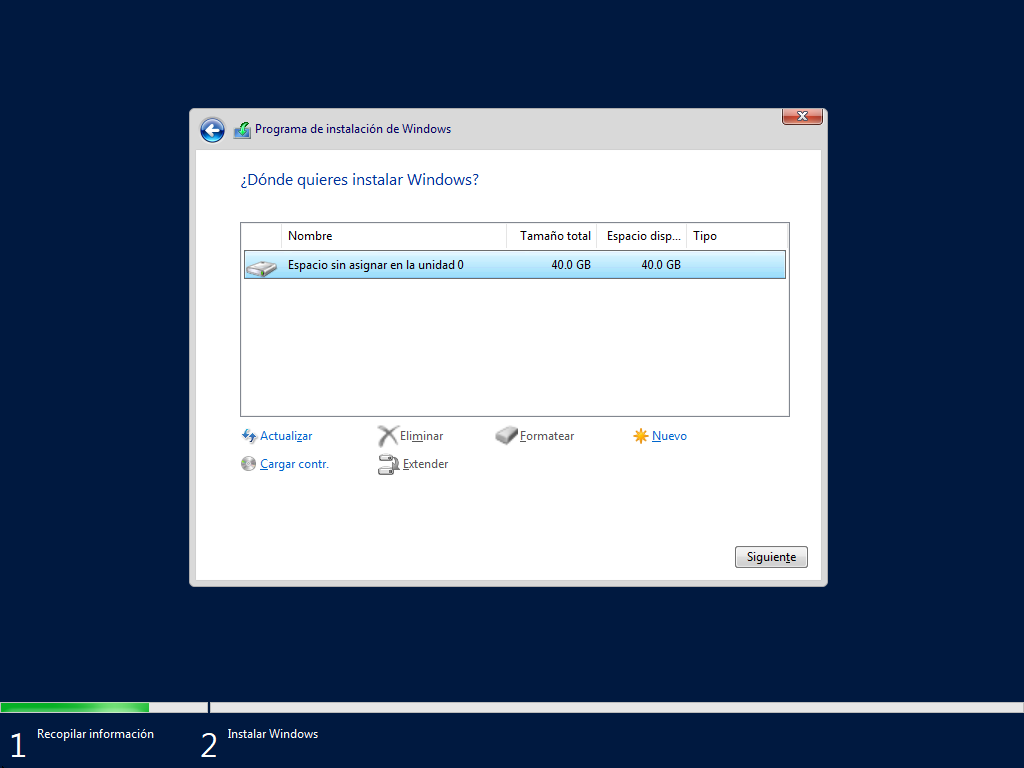
\includegraphics[trim={188 180 195 107},clip,width=\linewidth]{4_instalacion.png}
    \end{minipage}
}

\subsection{Terminar el proceso de instalación}
{
    \begin{minipage}{0.6\linewidth}
        \setlength{\parskip}{1.2em}
        Tras haber seleccionado y haber completado todos los pasos que se han descrito hasta ahora, el proceso de instalación comenzará.

        Este paso de la instalación requerirá de cierto tiempo que dependerá del hardware que tengamos disponible, ya que se realizará la copia de los ficheros de sistema, realizará las instalaciones pertinentes y por último instalará las actualizaciones necesarias.
    \end{minipage}
    \hfill
    \begin{minipage}{0.36\linewidth}
        \vspace{-11pt}
        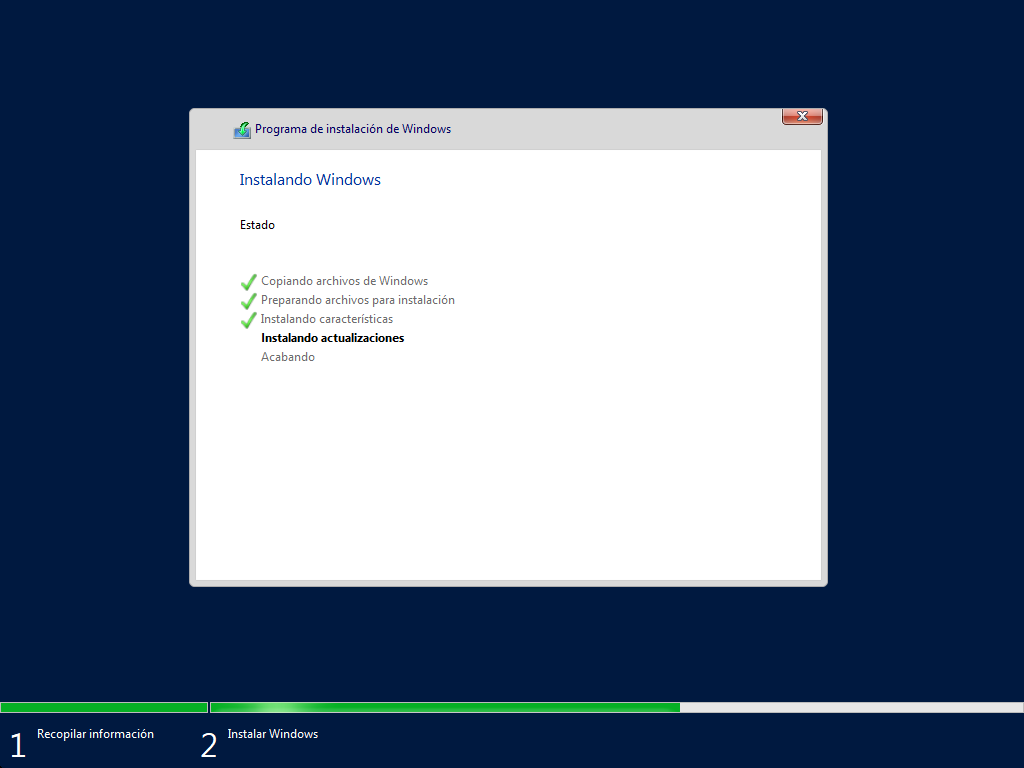
\includegraphics[trim={188 180 195 107},clip,width=\linewidth]{5_instalacion.png}
    \end{minipage}
}

\subsection{Personalizar la configuración}

{
    \begin{minipage}{0.6\linewidth}
        \setlength{\parskip}{1.2em}
        Al terminar el proceso anterior, el último paso nos permitirá realizar la configuración de la contraseña del usuario \textbf{Administrador}.

        Tal como se puede ver a continuación, el nombre de usuario no podrá ser modificado, y nos pedirá la contraseña y la confirmación de la contraseña.
    \end{minipage}
    \hfill
    \begin{minipage}{0.36\linewidth}
        \vspace{-11pt}
        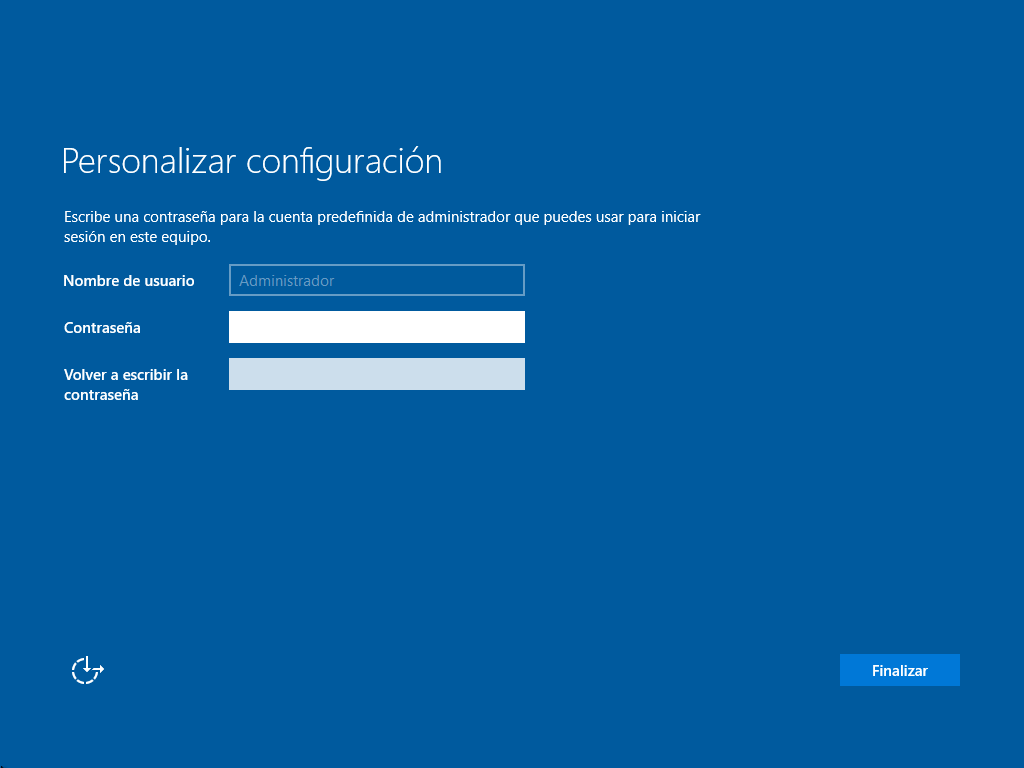
\includegraphics[trim={56 350 300 135},clip,width=\linewidth]{6_instalacion.png}
    \end{minipage}
}

Cabe recordar que esta contraseña es muy importante, ya que con ella realizaremos la configuración de todo el sistema, y por tanto debe ser una contraseña segura y debemos guardarla a buen recaudo. Al darle a “Finalizar” el servidor se reiniciará.

\section{Post-instalación}

Una vez realizada la instalación conviene retirar la imagen ISO del sistema de virtualización, así como incluso retirar el lector DVD virtual, ya que en principio no será necesario volverlo a usar.

Tras el primer arranque nos aparecerá la siguiente pantalla para realizar el login con el usuario Administrador, en donde introduciremos la contraseña que hemos puesto en el paso anterior. Una vez introducida, la siguiente pantalla será la pantalla de inicio donde podremos ver el panel de administrador del servidor.

\begin{tcolorbox}[title=Windows Server 2019 recién instalado,colback=white]
    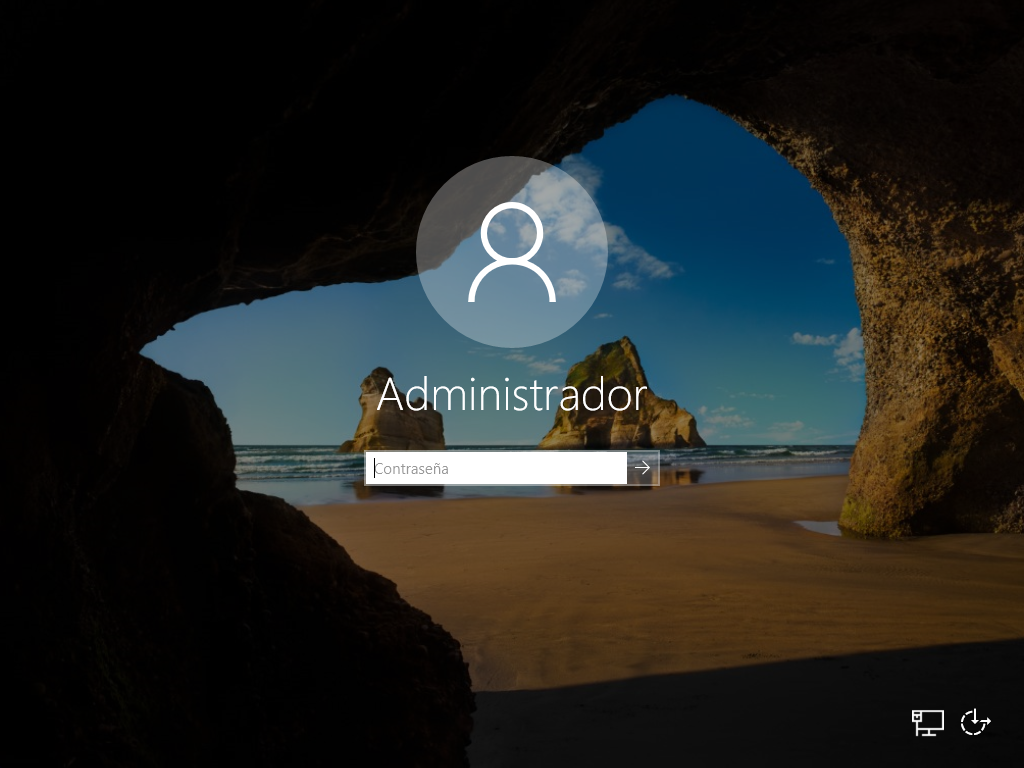
\includegraphics[width=0.48\linewidth]{7_instalacion.png}
    \hfill
    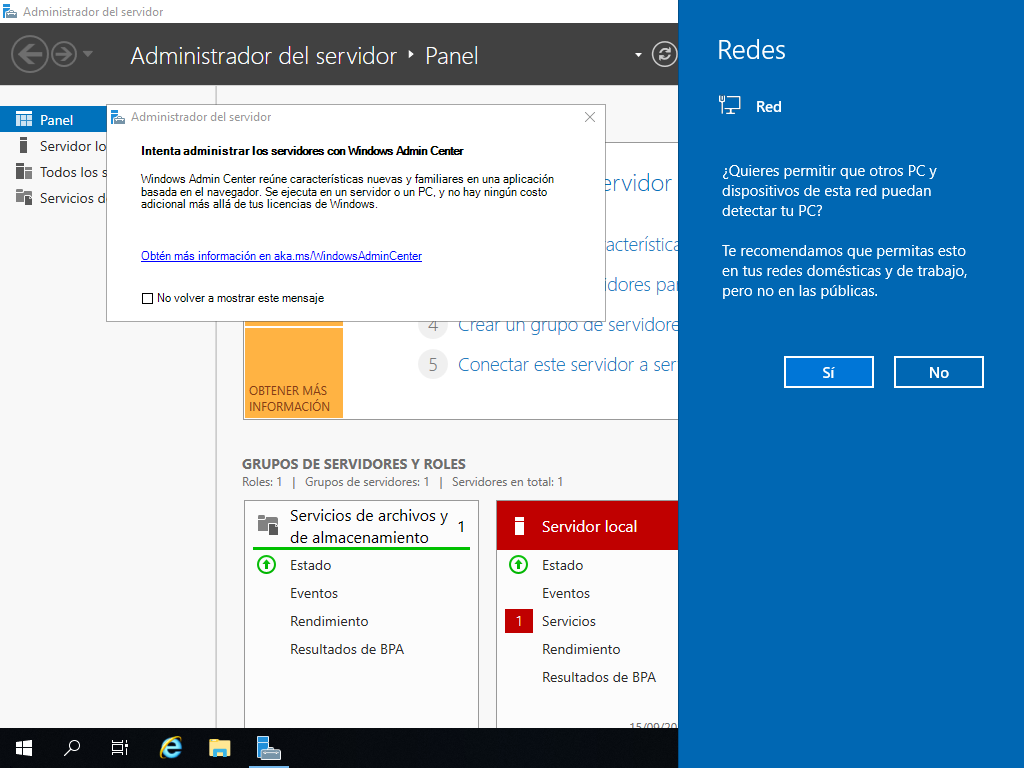
\includegraphics[width=0.48\linewidth]{8_instalacion.png}
\end{tcolorbox}


\chapter{Windows Server 2019 como servidor de red}
Windows Server 2019 tras la instalación no es más que un sistema operativo “normal”, que potencialmente se puede convertir en un Sistema Operativo de red, con funcionalidad para administrar usuarios, creación de grupos, permisos, … Para realizar estas funciones debemos de configurar el Sistema Operativo.

Como se ha observado, durante la instalación del Sistema Operativo apenas se realizan preguntas, por lo que es el propio instalador el que ha tomado ciertas decisiones por nosotros, como son:

\begin{itemize}
    \item Obtención de IP (a través de DHCP o Dynamic Host Configuration Protocol)
    \item Nombre del equipo
\end{itemize}

Estos datos los modificaremos más adelante.


\section{Entendiendo conceptos en Windows Server}
Durante la instalación y promoción del servidor como controlador de dominio y configuración de Active Directory, existen ciertos conceptos que son intrínsecos a cómo va a funcionar Windows Server como servidor  y que deben de ser entendidos.


\subsection{Active Directory}
\textbf{\textit{Active Directory}} (AD), o \textbf{Directorio Activo}, son los términos que utiliza Microsoft para referirse a su implementación de servicio de directorio en una red distribuida de computadores. Utiliza distintos protocolos, principalmente \href{https://es.wikipedia.org/wiki/Protocolo_ligero_de_acceso_a_directorios}{LDAP}, \href{https://es.wikipedia.org/wiki/Sistema_de_nombres_de_dominio}{DNS}, \href{https://es.wikipedia.org/wiki/Protocolo_de_configuraci%C3%B3n_din%C3%A1mica_de_host}{HDCP} y \href{https://es.wikipedia.org/wiki/Kerberos}{Kerberos}.

De forma sencilla se puede decir que es un servicio establecido en uno o varios servidores en donde se crean objetos tales como usuarios, equipos o grupos, con el objetivo de administrar los inicios de sesión en los equipos conectados a la red, así como también la administración de políticas en toda la red.

Su estructura jerárquica permite mantener una serie de objetos relacionados con componentes de una red, como usuarios, grupos de usuarios, permisos y asignación de recursos y políticas de acceso. (Fuente: \href{https://es.wikipedia.org/wiki/Active_Directory}{wikipedia}).


\subsection{Dominio}
Un dominio es una colección de objetos dentro del directorio que forman un subconjunto administrativo. Pueden existir diferentes dominios dentro de un bosque, cada uno de ellos con su propia colección de objetos y unidades organizativas.

Para poner nombre a los dominios se utiliza el protocolo DNS. Por este motivo, Active Directory necesita al menos un servidor DNS instalado en la red

\subsection{Unidad Organizativa (UO)}
En inglés Organizational Unit (OU). Es la unidad jerárquica inferior al dominio que puede tener objetos y/u otras UO. Más adelante las usaremos para la creación de GPOs.

\infobox{\textbf{Las Unidades Organizativas (UO) son contenedores dentro del Active Directory}}


\subsection{Objeto}
La palabra Objeto se utiliza como nombre genérico para referirnos a cualquiera de los componentes que forman parte del directorio, como una impresora o una carpeta compartida, pero también un usuario, un grupo, etc. Incluso podemos utilizar la palabra objeto para referirnos a una Unidad organizativa.

Cada objeto dispondrá de una serie de características específicas (según la clase a la que pertenezca) y un nombre que permitirá identificarlo de forma precisa. En general, los objetos se organizan en tres categorías:
\begin{itemize}
    \item \textbf{Usuarios}: identificados a través de un nombre (y, casi siempre, una contraseña), que pueden organizarse en grupos, para simplificar la administración.
    \item \textbf{Recursos}: que son los diferentes elementos a los que pueden acceder, o no, los usuarios según sus privilegios. Por ejemplo, carpetas compartidas, impresoras, etc.
    \item \textbf{Servicios}: que son las diferentes funciones a las que los usuarios pueden tener acceso. Por ejemplo, el correo electrónico.
\end{itemize}


\subsection{Controlador de dominio}
Un Controlador de Dominio (domain controller) contiene la base de datos de objetos del directorio para un determinado dominio, incluida la información relativa a la seguridad. Además, será responsable de la autenticación de objetos dentro de su ámbito de control.

En un dominio dado, puede haber varios controladores de dominio asociados, de modo que cada uno de ellos represente un rol diferente dentro del directorio. Sin embargo, a todos los efectos, todos los controladores de dominio, dentro del mismo dominio, tendrán la misma importancia.


\subsection{Árbol}
Un Árbol es simplemente una colección de dominios que dependen de una raíz común y se encuentran organizados como una determinada jerarquía. Dicha jerarquía también quedará representada por un espacio de nombres DNS común.

De esta forma, sabremos que los dominios \textbf{mikeldi.com} e \textbf{informatica.mikeldi.com} forman parte del mismo árbol, mientras que \textbf{mikeldi.com} y \textbf{linux.org} no.

Si un determinado usuario es creado dentro de un dominio, éste será reconocido automáticamente en todos los dominios que dependan jerárquicamente del dominio al que pertenece.


\subsection{Bosque}
El Bosque es el mayor contenedor lógico dentro de Active Directory, abarcando a todos los dominios dentro de su ámbito. Los dominios están interconectados por Relaciones de confianza transitivas que se construyen automáticamente (consultar más adelante el concepto de Relación de confianza). De esta forma, todos los dominios de un bosque confían automáticamente unos en otros y los diferentes árboles podrán compartir sus recursos.

\begin{center}
    \vspace{-15pt}
    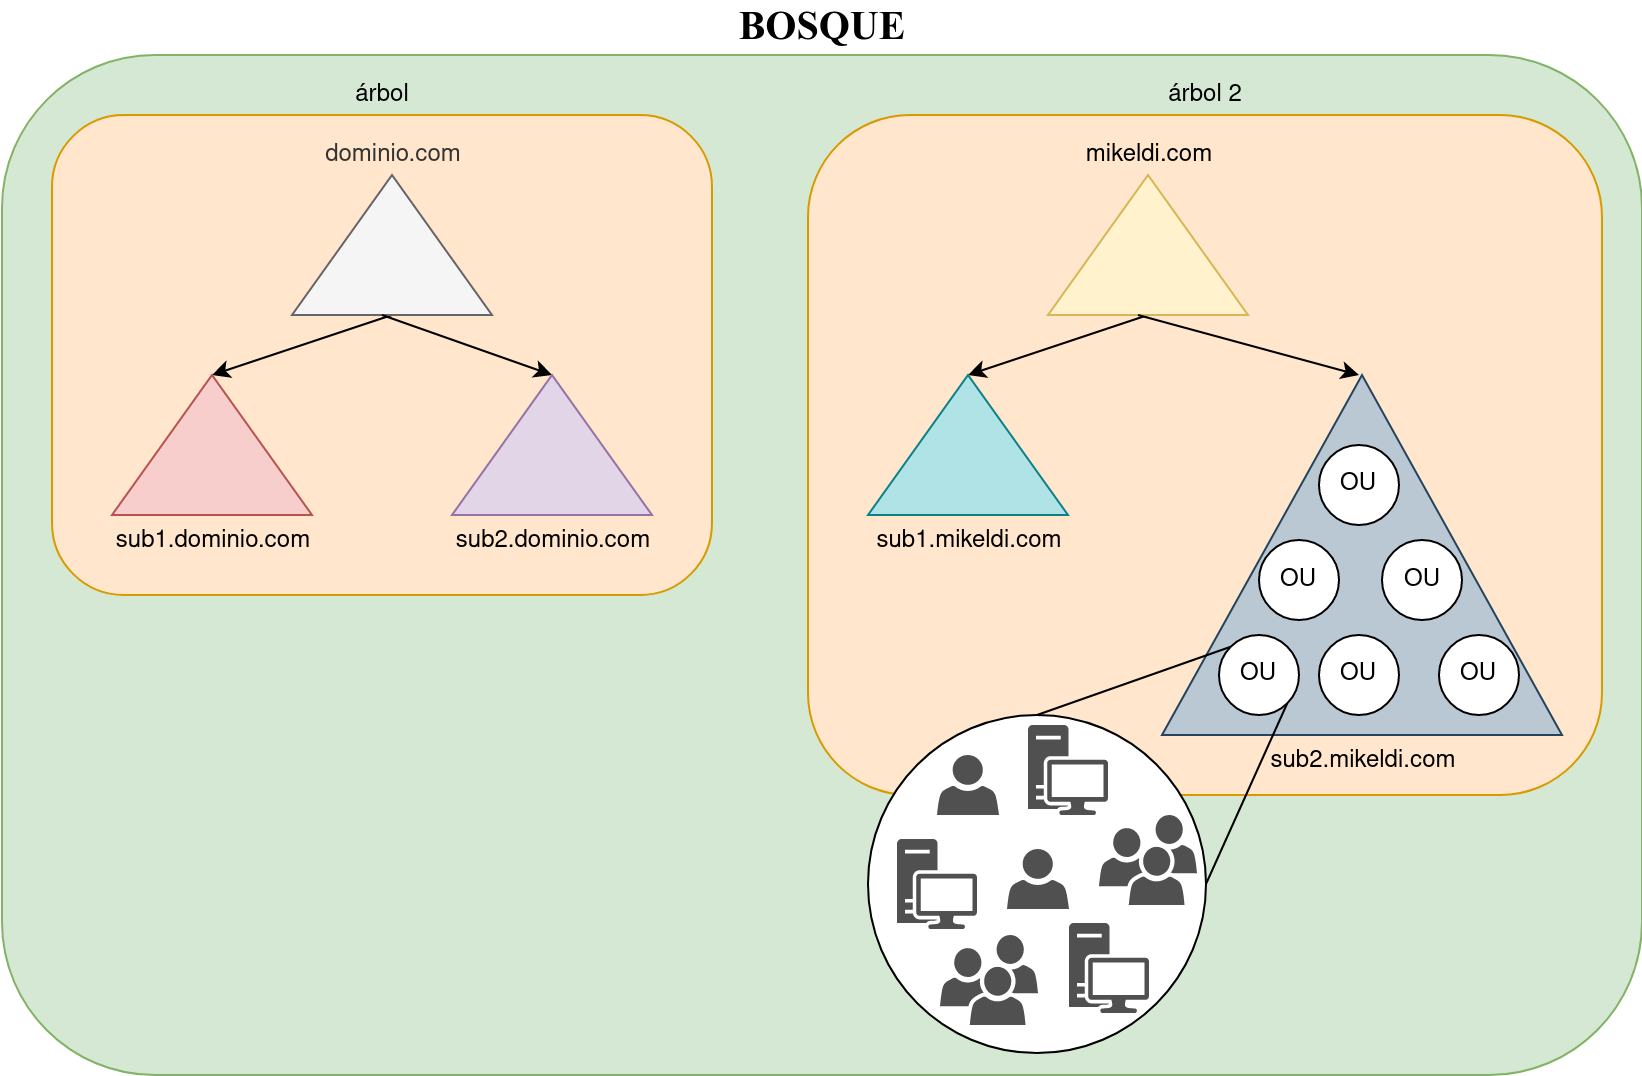
\includegraphics[width=0.6\linewidth]{bosque_directorio_activo.png}
    \vspace{-15pt}
\end{center}

Como ya hemos dicho, los dominios pueden estar organizados jerárquicamente en un árbol que comparte un espacio de nombres DNS común. A su vez, \textbf{diferentes árboles pueden estar integrados en un bosque}. Al tratarse de \textbf{árboles diferentes, no compartirán el mismo espacio de nombres}.

\subsection{Relaciones de confianza}
En el contexto de Active Directory, las Relaciones de confianza son un método de comunicación seguro entre dominios, árboles y bosques. Las relaciones de confianza permiten a los usuarios de un dominio del Directorio Activo autenticarse en otro dominio del directorio.


\section{Configurando Windows Server como servidor en Red}
Antes de promocionar el servidor a controlador de dominio, y por tanto convertirlo en un servidor en red, debemos realizar unos pasos previos de configuración. Los pasos que tendremos que realizar serán los siguientes:

\begin{itemize}
    \item Configurar una \textbf{IP estática} al equipo: Todos los servidores en una red (tanto pública como privada) debe de tener una IP estática en la misma. Deberemos de conocer el direccionamiento de la red, y confirmar que la IP que vamos a configurar no está siendo utilizada por otro equipo.
    \begin{itemize}
        \item El cambio de IP se realiza en “\textbf{Configuración de Red e Internet}”, en este caso “Protocolo de Internet versión 4” y poniendo la IP correspondiente a nuestra red.
        \begin{center}
            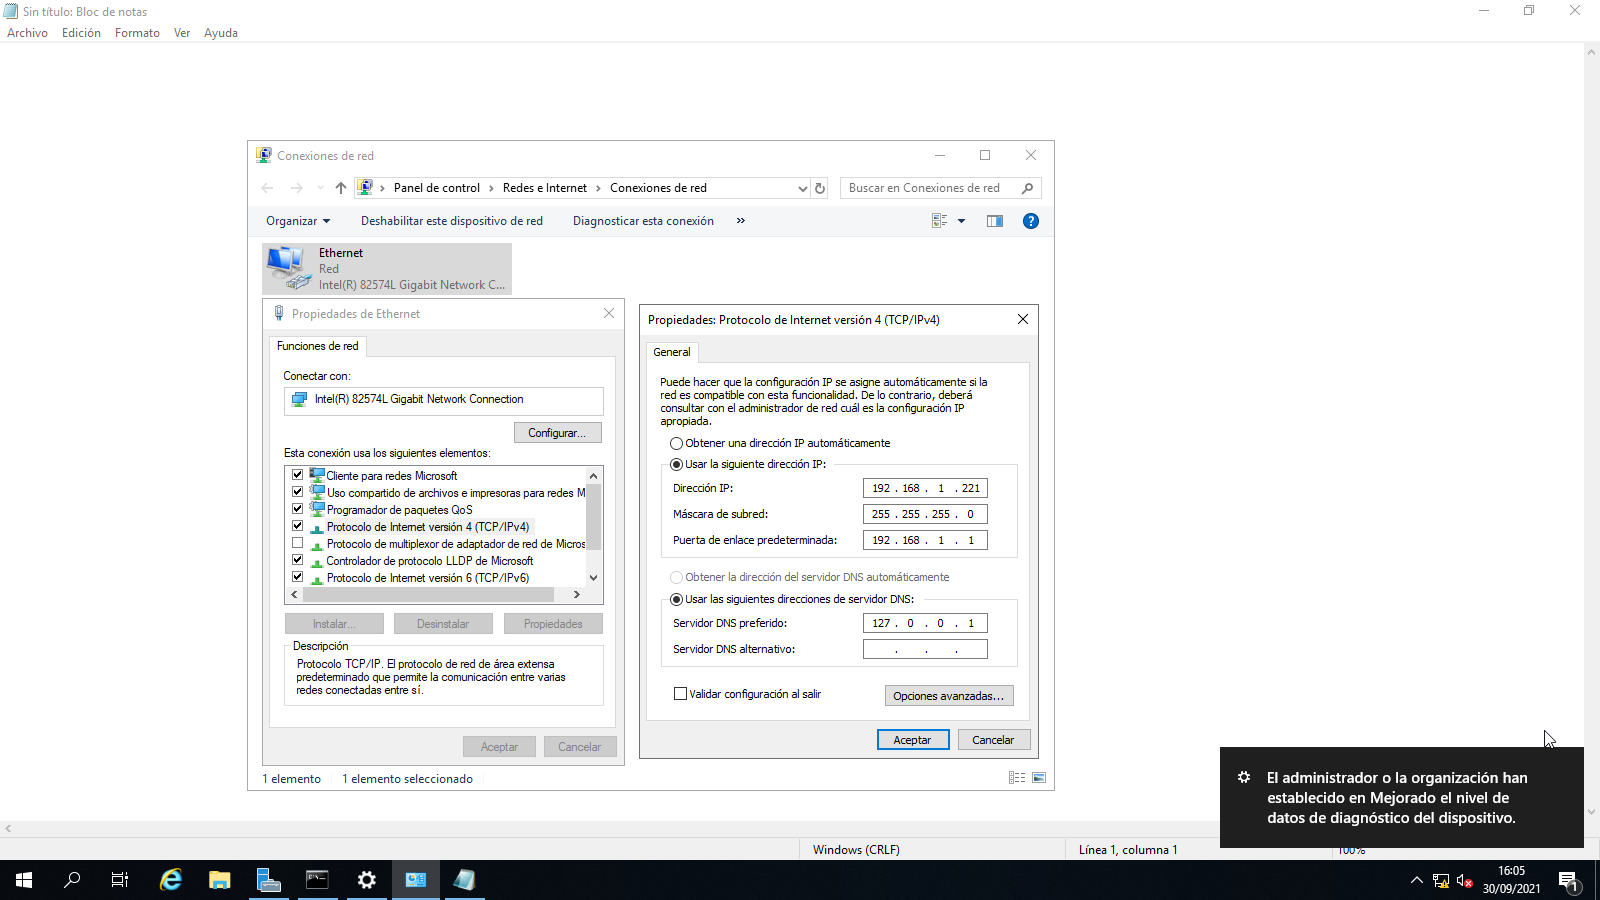
\includegraphics[trim={245 105 540 139},clip,width=0.8\linewidth]{cambiar_ip_windows.png}
        \end{center}
        \item También vamos a configurar como \textbf{Servidor DNS preferido} la IP localhost, “127.0.0.1”, para que posteriormente Active Directory ejerza de DNS local.
    \end{itemize}

    \hypertarget{cambiar_nombre_equipo}{}
    \item Cambiar el \textbf{nombre del equipo}: Para que los servidores sean fácilmente identificables, debemos proporcionarles un nombre de equipo que indique cuáles son sus funciones. En nuestro caso, podemos llamarlo “\textbf{AD}” (de Active Directory) o “\textbf{DC}” (de \textit{Domain Controller}). Tras realizar el cambio, el servidor deberá reiniciarse. El cambio se puede realizar desde varias partes de Windows Server, como por ejemplo:
    \begin{itemize}
        \item Click derecho en Inicio → Sistema
        \item Panel de control → Sistema y Seguridad → Sistema → Cambiar Configuración
    \end{itemize}
    \begin{center}
        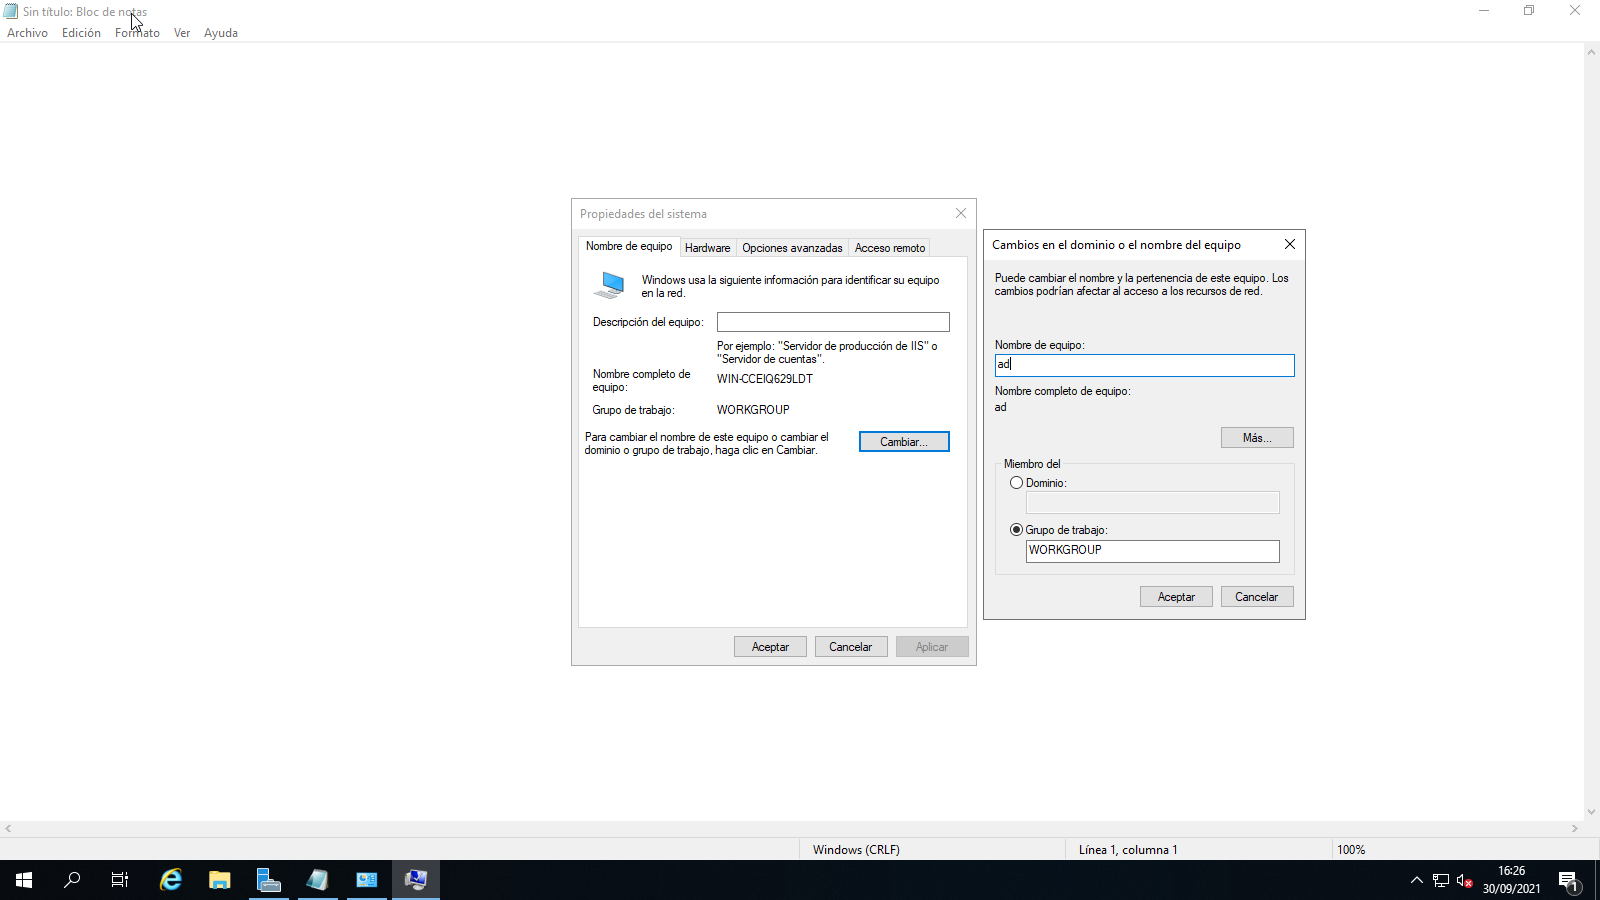
\includegraphics[trim={568 230 290  195},clip,width=0.8\linewidth]{cambiar_nombre_windows.png}
    \end{center}

    \item Asegurar que la zona horaria es la adecuada
    \begin{itemize}
        \item Comprobar servicio de hora
        \item Comprobar que la actualización de la hora es automática
    \end{itemize}

\end{itemize}


\section{Instalar Active Directory}
Para promocionar el servidor a controlador de dominio de Active Directory debemos de realizar la instalación del rol. Para ello, iremos al “\textbf{Administrador del Servidor}”.

\begin{center}
    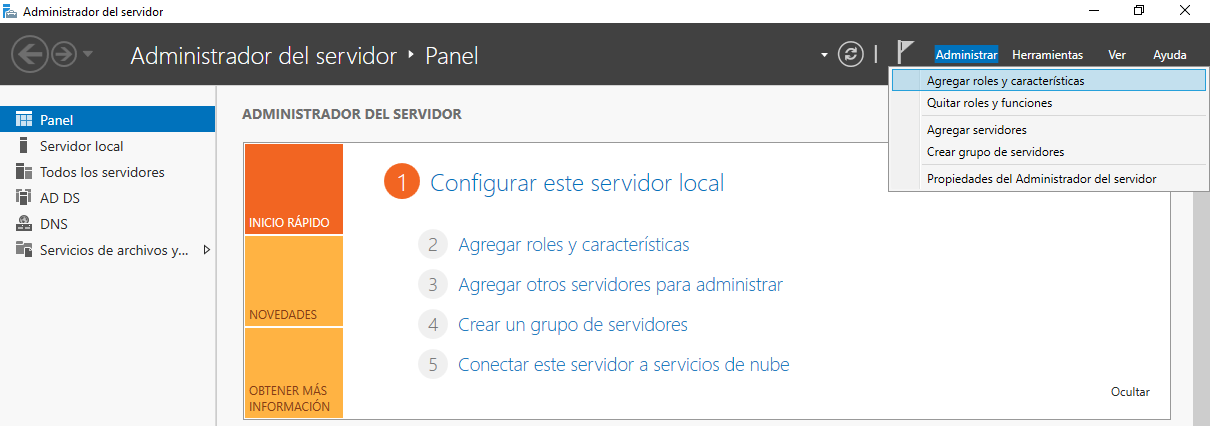
\includegraphics[frame,width=0.8\linewidth]{administrador_del_servidor.png}
\end{center}

Haremos click en “Administrar”, “Agregar roles y características” y nos saldrá una nueva ventana, con un aviso del asistente y al darle a “Siguiente”, elegiremos la primera opción, “\textbf{Instalación basada en características y roles}” y volveremos a darle a “Siguiente” en el asistente:

\begin{center}
    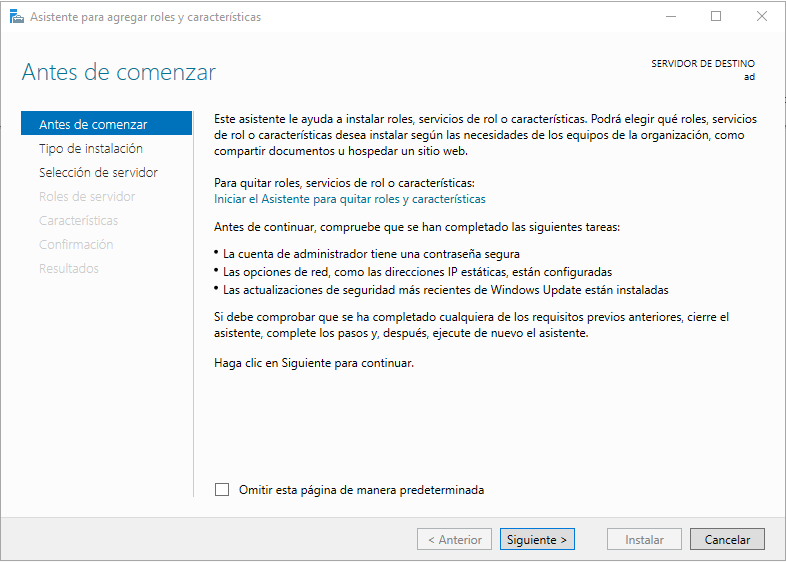
\includegraphics[width=0.46\linewidth]{active_directory_1.png}
    \hfill
    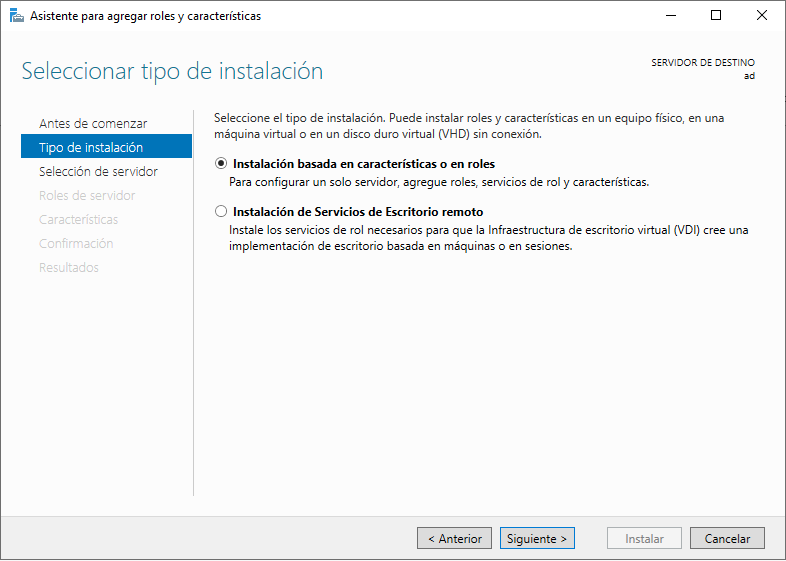
\includegraphics[width=0.46\linewidth]{active_directory_2.png}
\end{center}

{
    \begin{minipage}{0.6\linewidth}
        \setlength{\parskip}{1.2em}
        El siguiente paso será elegir el servidor dónde queremos realizar la instalación del rol de Active Directory. De primeras, puede parecer raro que nos pregunte en dónde queremos realizar la instalación, pero es fácil de entender cuando desde un servidor podremos llegar a controlar otros. De momento, sólo nos aparecerá el propio servidor donde estamos realizando la instalación, por lo que lo dejamos seleccionado y le damos a “Siguiente”.
    \end{minipage}
    \hfill
    \begin{minipage}{0.36\linewidth}
        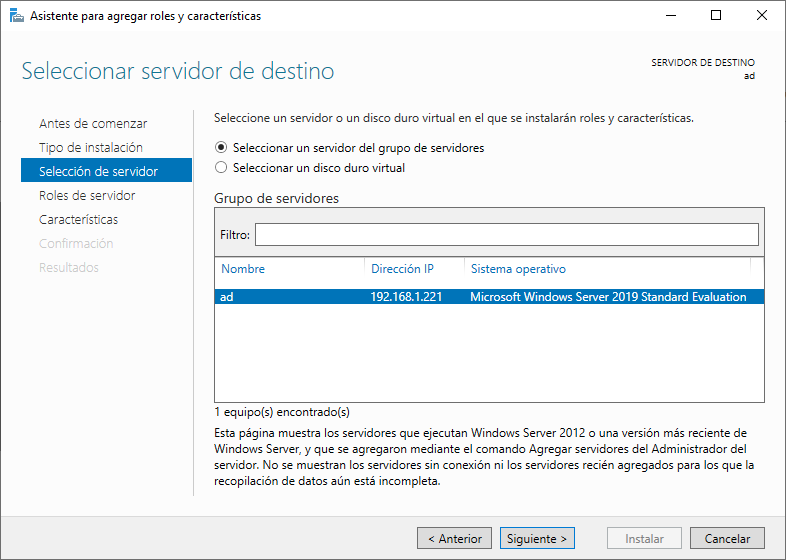
\includegraphics[width=\linewidth]{active_directory_3.png}
    \end{minipage}
}

En el siguiente apartado podremos realizar la elección del rol que queremos añadir a nuestro servidor, y en este caso deberemos hacer click y asegurarnos que la opción está seleccionada en la opción “\textbf{Servicios de dominio de Active Directory}”.


\begin{center}
    \vspace{-15pt}
    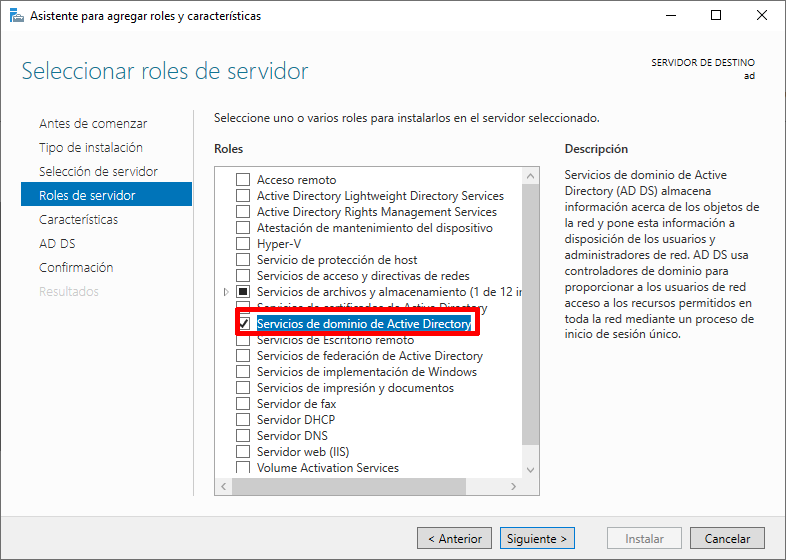
\includegraphics[width=0.6\linewidth]{active_directory_4.png}
    \vspace{-15pt}
\end{center}

Al hacer click en ella, nos saldrá una nueva ventana en la que nos avisa que se van a añadir herramientas necesarias para este rol, por lo que le daremos a “Agregar características” en esa nueva ventana. Le daremos a “Siguiente” para pasar al siguiente paso de la instalación.

El siguiente paso es el de “\textbf{Características}”, en la que aparecen distintas opciones con su descripción. De momento no vamos a realizar ninguna instalación en este apartado. Le daremos a Siguiente.

En el último paso nos aparecerá una confirmación de los pasos que se van a realizar y sólo nos quedará darle a “\textbf{Instalar}”:

\begin{center}
    \vspace{-15pt}
    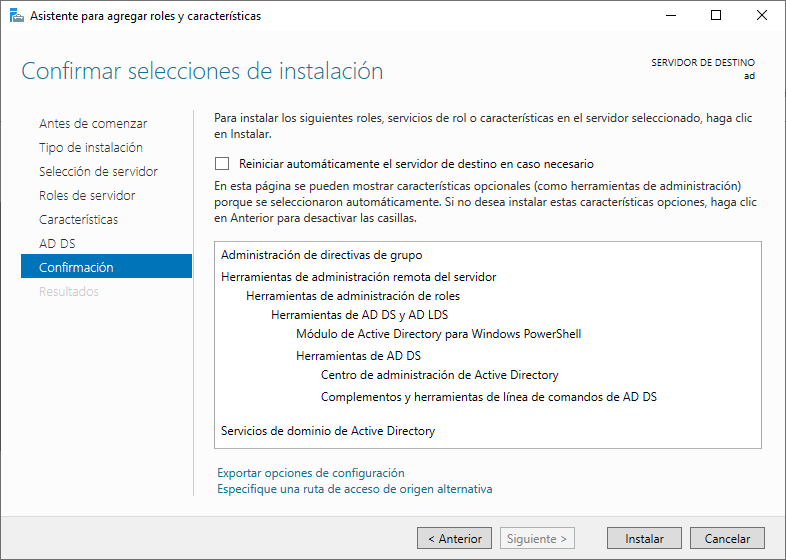
\includegraphics[width=0.8\linewidth]{active_directory_5.png}
    \vspace{-15pt}
\end{center}

Tras esperar unos segundos, el proceso terminará y el botón de “Instalar” se cambiará por el de “Cerrar”.

\section{Configurar Active Directory}
Tras realizar la instalación del rol de \textbf{Active Directory} en nuestro Windows Server, aparecerá un mensaje en la consola de administrador para que realicemos la configuración del mismo.

\begin{center}
    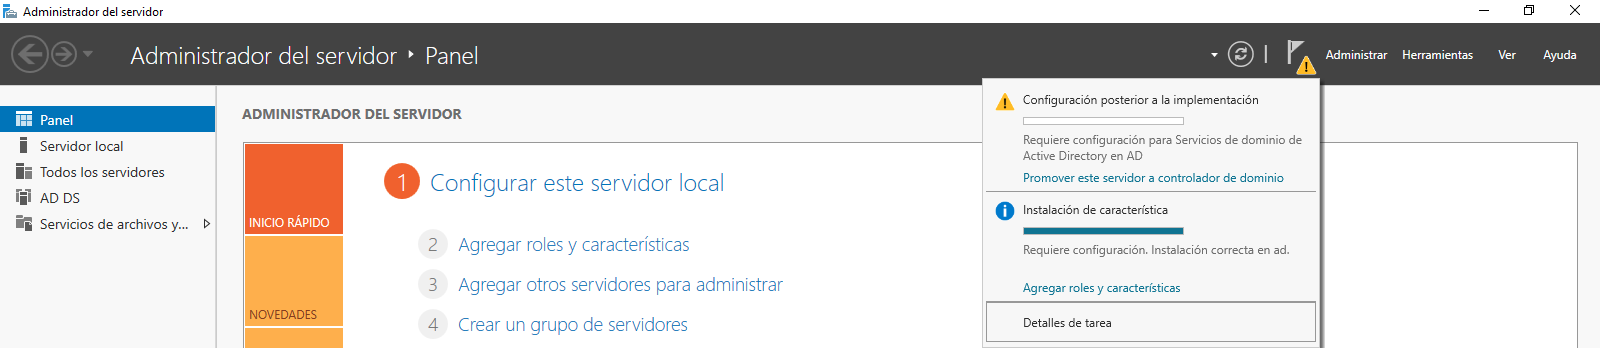
\includegraphics[frame,width=\linewidth]{configurar_active_directory_1.png}
\end{center}

En el desplegable haremos click en “\textbf{Promover este servidor a controlador de dominio}”, y nos abrirá una nueva ventana en la que tendremos que realizar una serie de pasos para realizar la configuración del Active Directory recién instalado.


\subsection{Tipos de implementación}
En el primer paso a la hora de configurar Active Directory aparecen tres opciones distintas que debemos de entender antes de proceder con la configuración. En la siguiente pantalla aparecen las tres opciones:

\begin{center}
    \vspace{-15pt}
    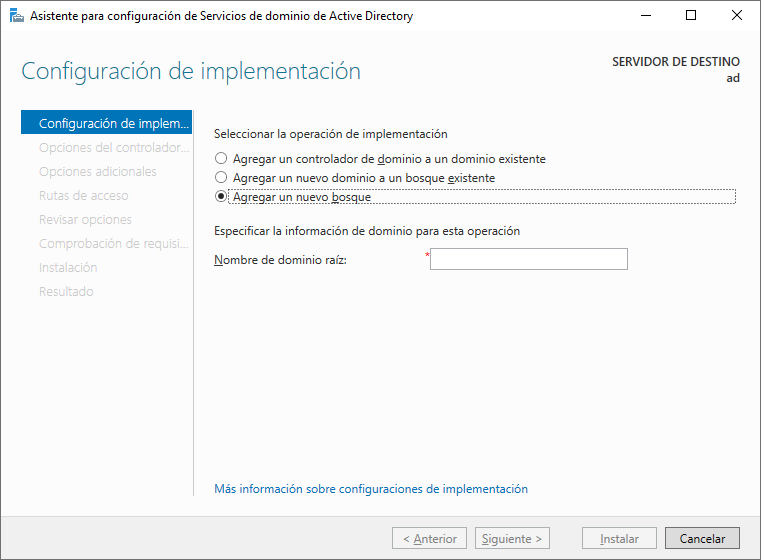
\includegraphics[width=0.6\linewidth]{configurar_active_directory_2.png}
    \vspace{-15pt}
\end{center}

\begin{itemize}
    \item \textbf{Agregar un controlador de dominio a un dominio existente}: lo utilizaremos cuando queramos tener Alta Disponibilidad en nuestra infraestructura, ya que el nuevo servidor actuará de réplica del servidor que actúe de controlador actualmente.
    \item \textbf{Agregar un dominio a un bosque existente}: cuando necesitemos añadir un nuevo dominio (para realizar diferenciación a otro que ya tengamos instalado) a un bosque ya existente.
    \item \textbf{Agregar un nuevo bosque}: Utilizado para realizar instalaciones nuevas creando un nuevo dominio.
\end{itemize}

\subsection{Nombre de dominio raíz}
A la hora de elegir un dominio para nuestro Active Directory existen varias opciones:

\begin{itemize}
    \item Elegir un \textbf{TLD} (Top Level Domain) válido, registrado a tu empresa. Ejemplo: \textbf{mikeldi.com}
    \item Usar un \textbf{subdominio de un TLD} válido. Ejemplo: corp.mikeldi.com
    Usar un \textbf{TLD no válido}. Ejemplo: mikeldi.local, mikeldi.corp, …
    \item En principio, y salvo que tengamos una razón para ello, elegiremos la primera opción y le daremos al botón de “Siguiente”.
\end{itemize}

Dado que estamos realizando una instalación nueva, utilizaremos la última opción.

\subsection{Opciones del controlador de dominio}
En el siguiente paso de configuración del Active Directory tendremos distintas opciones que debemos entender para proceder a su configuración:

\begin{center}
    \vspace{-15pt}
    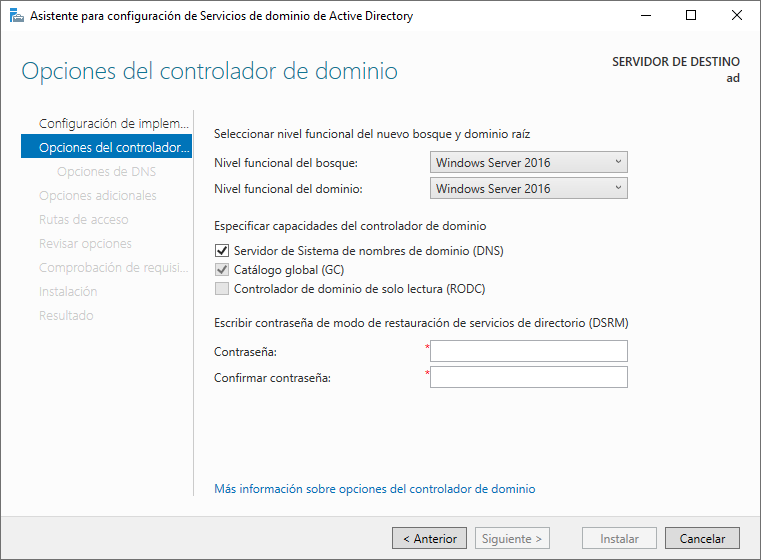
\includegraphics[width=0.6\linewidth]{configurar_active_directory_3.png}
    \vspace{-15pt}
\end{center}

Los niveles funcionales determinan las funcionalidades disponibles de dominio o bosque de Active Directory, y determinan los sistemas operativos Windows Server que se pueden ejecutar en los controladores. Normalmente, \textbf{deberíamos elegir las últimas versiones disponibles} para poder utilizar el mayor número de características posibles. En caso de que necesitemos compatibilidad con  versiones anteriores, entonces elegiremos la versión correspondiente.

También nos va a pedir la contraseña de restauración de servicios de directorio DSRM. Con ella podremos iniciar sesión cuando no se esté ejecutando el servicio de Active Directory, ya sea porque se ha detenido o porque hemos tenido que iniciar en modo DSRM el servidor.


\subsection{Otras opciones}
Una vez realizado el paso anterior, y tras darle a “Siguiente”, nos aparecerán nuevos pasos que podremos pasarlos sin realizar modificaciones, ya que las configuraciones por defecto se corresponden al dominio que hayamos introducido o rutas donde se almacena la información. El último paso será para revisar y realizar la instalación:

\begin{center}
    \vspace{-15pt}
    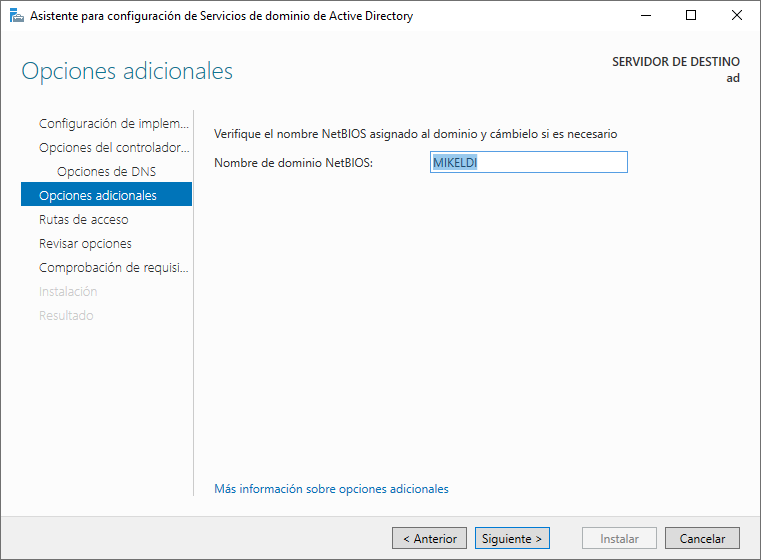
\includegraphics[width=0.32\linewidth]{configurar_active_directory_4.png}
    \hfill
    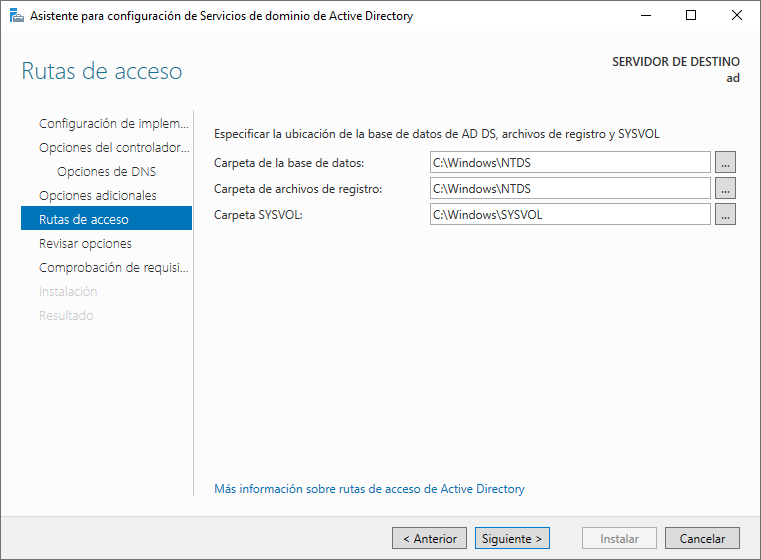
\includegraphics[width=0.32\linewidth]{configurar_active_directory_5.png}
    \hfill
    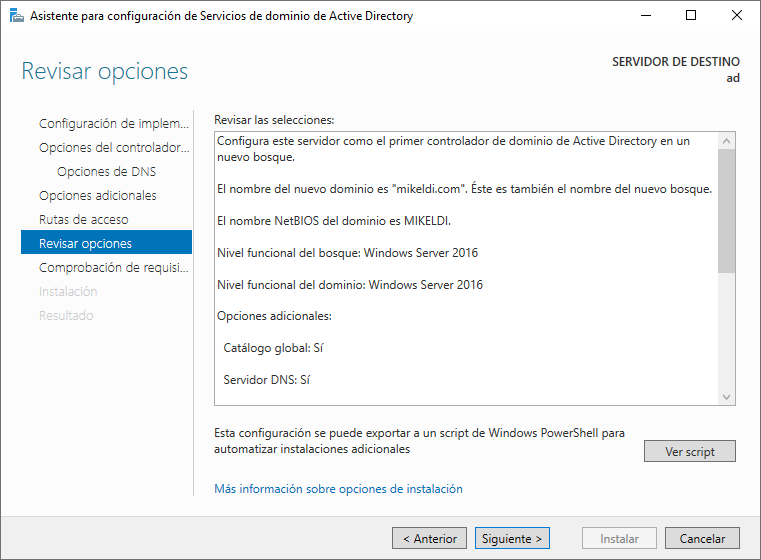
\includegraphics[width=0.32\linewidth]{configurar_active_directory_6.png}
    \vspace{-15pt}
\end{center}

Tras estos pasos revisaremos las opciones y le daremos a “Instalar”.

\chapter{Añadir un equipo Windows 10 al dominio}
Tras seguir los pasos previos, podremos añadir equipos al dominio creado en Active Directory y hacer uso de las configuraciones, usuarios y restricciones que iremos creando en apartados sucesivos. Para que un equipo Windows pueda pertenecer a un Active Directory debe ser de la familia “\textbf{Pro}”, como por ejemplo: Windows 7 Pro, Windows 10 Pro…

\section{Instalación de Windows 10 Pro}
Para realizar la instalación de un equipo con Windows 10, podremos hacer uso de la ISO que podremos descargar desde la página de Microsoft.


{
    \begin{minipage}{0.68\linewidth}
        \setlength{\parskip}{1.2em}
        No se van a explicar todos los pasos, ya que el sistema de instalación es sencillo. El único apartado donde deberemos fijarnos es en la pantalla de la derecha.

        Tal como se ve en la imagen, elegiremos la opción “Windows 10 Pro”, y continuaremos.
    \end{minipage}
    \hfill
    \begin{minipage}{0.3\linewidth}
        \vspace{-15pt}
        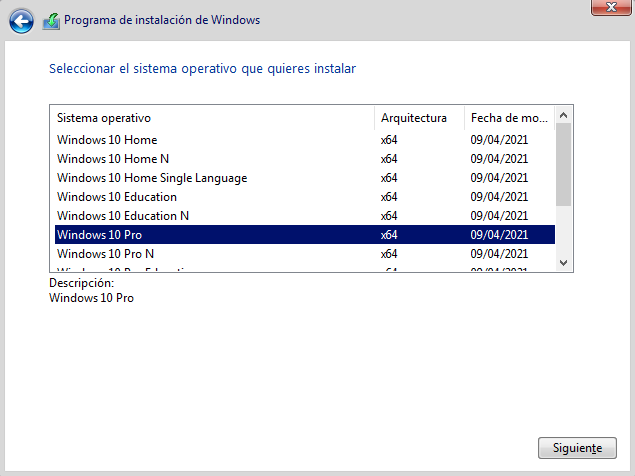
\includegraphics[width=\linewidth]{windows_10_1.png}
    \end{minipage}
}

Al finalizar la instalación, el equipo se reiniciará y podremos introducir el usuario y contraseña que hemos creado durante la instalación.

\infobox{\textbf{El usuario creado en la instalación es una cuenta LOCAL del equipo}}

\section{Pasos previos}
El equipo Windows 10 Pro deberá estar situado en la misma red del Windows Server, o permitir todas las conexiones que sean necesarias de estar en otra red.

Es recomendable modificar el nombre del equipo para que posteriormente sea más fácil de encontrarlo dentro del Active Directory, ya que el nombre por defecto de instalación es aleatorio. Para realizar el cambio, podremos seguir los \hyperlink{cambiar_nombre_equipo}{pasos indicados previamente para Windows Server}, y en este caso elegiremos el nombre “win10”.

Y por último, en la configuración de red del equipo Windows 10 configuraremos el servidor DNS preferido para que sea la IP del Windows Server 2019. Este cambio se podría realizar de manera automática si modificamos la configuración del DHCP de la red.

\begin{center}
    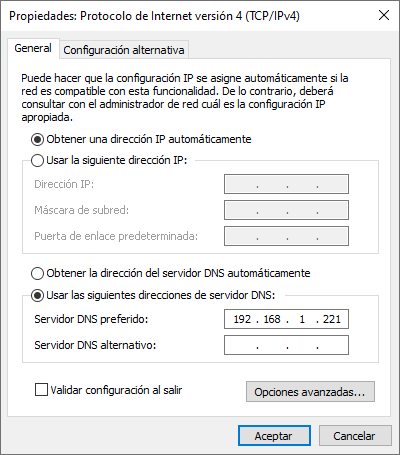
\includegraphics[trim={20 90 21 287},clip,width=0.5\linewidth]{windows_10_2.png}
\end{center}

\section{Añadir el equipo al dominio}
Tras realizar los pasos previos, para añadir un equipo a un dominio de Active Directory tendremos que ir a la \textbf{Propiedades del Sistema} de Windows (dependiendo de la versión de Windows se puede llegar a esta pantalla de varias maneras).

Le daremos a “Cambiar”. Si no hemos cambiado el nombre al equipo, podremos hacerlo en la nueva ventana, y a la par seleccionaremos el “Dominio” que hemos creado previamente, le daremos a “Aceptar” y nos aparecerá una nueva ventana donde \textbf{introduciremos el usuario “Administrador” y contraseña del Windows Server 2019}.

{
    \begin{minipage}{0.3\linewidth}
        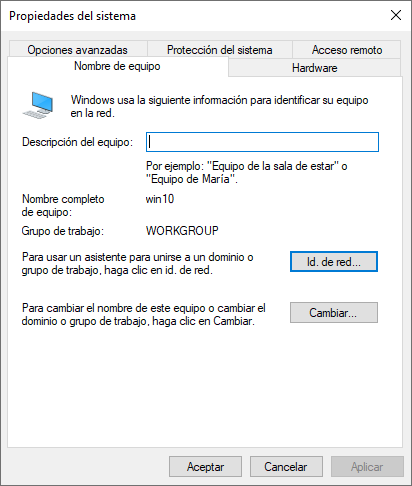
\includegraphics[width=\linewidth]{windows_10_meter_dominio_1.png}
    \end{minipage}
    \hfill
    \begin{minipage}{0.3\linewidth}
        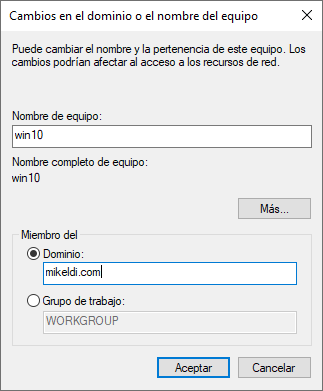
\includegraphics[width=\linewidth]{windows_10_meter_dominio_2.png}
    \end{minipage}
    \hfill
    \begin{minipage}{0.3\linewidth}
        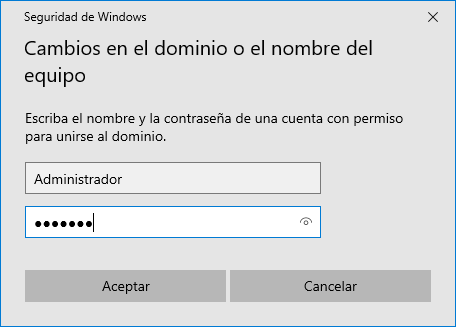
\includegraphics[width=\linewidth]{windows_10_meter_dominio_3.png}
    \end{minipage}
}

El equipo se conectará al servidor Windows Server 2019, comprobará que los datos son correctos, añadirá el equipo al Active Directory y nos pedirá reiniciar.


\section{Diferenciar usuario local y usuario de Active Directory}
Una vez que el equipo Windows 10 se ha añadido al Active Directory, nos vamos a poder loguear a él de dos maneras distintas:

\begin{itemize}
    \item \textbf{Usuario local}: Tras la instalación de Windows 10 sólo existe un usuario, que es el que hemos creado durante la instalación y es \textbf{Administrador local}. Este usuario no deberíamos utilizarlo salvo que el equipo tuviese algún problema que no se pudiese solventar desde Windows Server, quizá porque se haya salido del dominio, no tiene conexión a la red, …
    \item \textbf{Usuario de Active Directory}: La gestión de usuarios va a ser centralizada en Active Directory tal como vamos a ver en el apartado de gestión de grupos y usuarios, por lo que cualquier usuario que sea creado en Active Directory ahora mismo podría hacer login en este equipo.
\end{itemize}

A partir de ahora, cuando nos vuelva a salir la pantalla para introducir el usuario y contraseña, nos aparecerá a la izquierda el usuario que hayamos creado durante la instalación de Windows 10 y la opción “\textbf{Otro Usuario}”. Al seleccionar esta opción, tendremos que introducir un usuario y la contraseña de un usuario \textbf{que exista en Active Directory}.

\begin{center}
    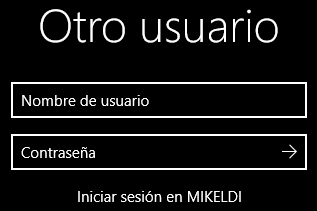
\includegraphics[width=0.3\linewidth]{windows_10_meter_dominio_4.png}
\end{center}

Tal como se puede ver, ya nos viene marcado que al introducir el usuario se va a iniciar la sesión en el dominio creado anteriormente. También podremos indicar lo siguiente como nombre de usuario:

\begin{itemize}
    \item \textbf{usuario@mikeldi.com}: cuando necesitemos iniciar sesión con “usuario” del dominio “mikeldi.com”.
    \item \textbf{ruben@dominio.com}: cuando queramos usar como inicio de sesión el usuario “ruben” del dominio “dominio.com”.
    \item \textbf{.\textbackslash{mikeldi}}: donde el punto hace referencia a iniciar sesión local y “mikeldi” es el usuario administrador local que hemos creado durante la instalación.
\end{itemize}

\chapter{Gestión de grupos y usuarios}
Para crear usuario y grupos, dentro del “\textbf{Administrador del Servidor}”, en el desplegable “\textbf{Herramientas}”, elegiremos la opción “\textbf{Usuarios y equipos de Active Directory}”, y nos aparecerá la siguiente ventana:

\begin{center}
    \vspace{-15pt}
    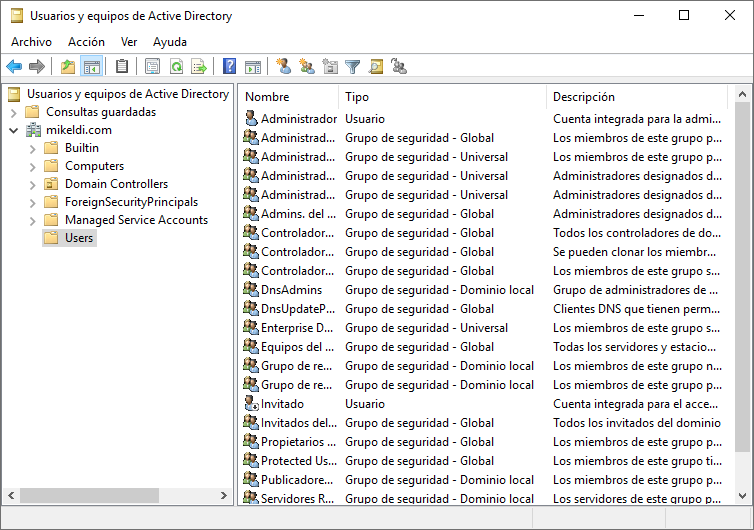
\includegraphics[width=0.7\linewidth]{configurar_active_directory_7.png}
\end{center}

Tal como se puede observar, a la izquierda tenemos un desplegable del dominio que hemos creado durante la instalación de Active Directory, y al seleccionar “Users” nos aparece a la derecha los \textbf{usuarios}  y \textbf{grupos de seguridad} que el sistema ha creado por defecto.

\section{Grupos dentro del Active Directory}
Los grupos dentro del Active Directory son objetos que \textbf{pueden contener usuarios, contactos, equipos u otros grupos}.

\warnbox{\textbf{No hay que confundir grupos con las Unidades Organizativas.}}

Al agregar un objeto a un grupo, ese objeto recibe todos los derechos asignados al grupo y todos los permisos asignados al grupo para todos los recursos compartidos.

Podemos utilizar los grupos para simplificar algunas tareas, como:

\begin{itemize}
    \item \textbf{Simplificar la administración}: Podemos asignar permisos al grupo y éstos afectarán a todos sus miembros.
    \item Delegar la \textbf{administración}: Podemos utilizar la directiva de grupo para asignar derechos de usuario una sola vez y, más tarde, agregar los usuarios a los que queramos delegar esos derechos.
    \item \textbf{Crear listas de distribución de correo electrónico}: Sólo se utilizan con los grupos de distribución que comentaremos más abajo.
\end{itemize}

Para crear grupos debemos tener clara la infraestructura de la empresa, los usuarios que tenemos y los grupos a los que va a pertenecer cada usuario. Esto es importante ya que la organización de los usuarios es una labor tediosa que en caso de tener que rehacerse se pierde tiempo en realizarlo.

Por otro lado, hay que recordar que cuando creemos el grupo el nombre será único dentro del dominio.


\subsection{Tipos de grupos}
Windows Server admite dos tipos de grupos:

\begin{itemize}
    \item \textbf{Distribución}: Se usa para crear listas de distribución de correo electrónico. Sólo se pueden usar con aplicaciones de correo electrónico (como Exchange Server) para enviar correo electrónico a colecciones de usuarios. Los grupos de distribución no tienen seguridad habilitada.
    \item \textbf{Seguridad}: Se usan para proporcionar de manera eficaz la asignación del acceso a los recursos de la red. Con los grupos de seguridad se pueden asignar derechos de usuario a grupos de seguridad en Active Directory permisos a grupos de seguridad de recursos.
\end{itemize}

\subsection{Ámbito de grupos}
Los grupos se caracterizan por un \textbf{ámbito} que identifica el grado en el que se aplica el grupo en el árbol de dominios o en el bosque. \textbf{El ámbito del grupo define dónde se pueden conceder permisos al grupo}. Los siguientes tres ámbitos de grupo se definen mediante Active Directory:

\begin{itemize}
    \item \textbf{Dominio Local}: Sólamente se puede otorgar permisos sobre los recursos que se sitúan en el dominio donde está ubicado el grupo de dominio local.
    \item \textbf{Global}: Puede otorgar permisos sobre los recursos de cualquier dominio del bosque, o dominios de confianza.
    \item \textbf{Universal}: Puede otorgar permisos sobre cualquier dominio del mismo bosque o de bosques de confianza.
\end{itemize}

\subsection{Grupos de seguridad predeterminados}
Los grupos predeterminados, como el grupo administradores del dominio, son grupos de seguridad que se crean automáticamente al crear un dominio en Active Directory. Se pueden utilizar estos grupos predefinidos para controlar el acceso a los recursos compartidos y para delegar roles administrativos específicos para todo el dominio.

A muchos grupos predeterminados se les asigna automáticamente un conjunto de derechos de usuario que autorizan a los miembros del grupo a realizar acciones específicas en un dominio, cómo iniciar sesión en un sistema local o realizar copias de seguridad de archivos y carpetas. Por ejemplo, un miembro del grupo operadores de copia de seguridad tiene el derecho de realizar operaciones de copia de seguridad para todos los controladores de dominio del dominio.

Los grupos predeterminados se encuentran en el contenedor \textbf{Builtin} y en el contenedor usuarios de usuarios y equipos de Active Directory.


\subsection{Crear un grupo para usuarios}
Windows Server ya trae una serie de grupos creados por defecto y cada uno de ellos cuenta con sus características.

Para crear un grupo propio tendremos que ir a “\textbf{Usuarios y equipos de Active Directory}”, seleccionar \textbf{Users} y hacer click derecho para elegir “\textbf{Nuevo}”:

\begin{center}
    \vspace{-10pt}
    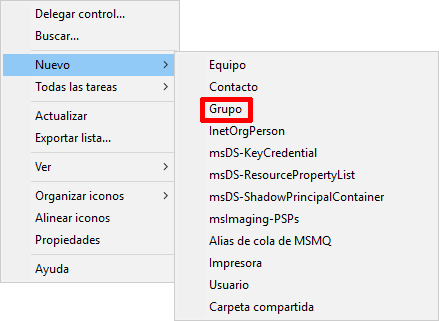
\includegraphics[width=0.5\linewidth]{crear_grupo.png}
    \vspace{-10pt}
\end{center}

Al darle a la opción “Grupo” tal como aparece en el menú desplegable, nos aparecerá una nueva ventana donde podremos elegir el nombre del grupo y las opciones comentadas previamente: qué “Ámbito de grupo” queremos que sea y el “Tipo de grupo”:

\begin{center}
    \vspace{-10pt}
    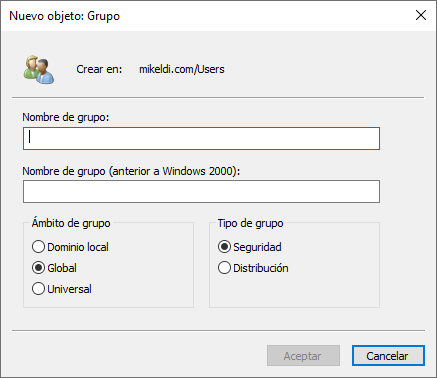
\includegraphics[width=0.5\linewidth]{crear_grupo2.png}
    \vspace{-10pt}
\end{center}

Tras poner las opciones que mejor nos convenga, nos aparecerá el nuevo grupo, al que posteriormente podremos añadir usuarios.

\section{Usuarios}
En Windows Server, una cuenta de usuario es un objeto que posibilita el acceso a los recursos del dominio de dos modos diferentes:

\begin{itemize}
    \item Permite \textbf{autenticar la identidad de un usuario}, porque sólo podrán iniciar una sesión aquellos usuarios que dispongan de una cuenta en el sistema asociada a una determinada contraseña.
    \item Permite \textbf{autorizar}, o \textbf{denegar}, el acceso a los recursos del dominio, porque, una vez que el usuario haya iniciado su sesión sólo tendrá acceso a los recursos para los que haya recibido los permisos correspondientes.
\end{itemize}

Cada cuenta de usuario dispone de un \textbf{identificador} de seguridad (\textbf{SID} o Security IDentifier) \textbf{que es único en el dominio}.


\subsection{Usuarios predeterminados}
Cuando se crea el dominio, se crean también dos nuevas cuentas:

\begin{itemize}
    \item \textbf{Administrador}: Tiene control total sobre el dominio y no se podrá eliminar ni retirar del grupo Administradores (aunque sí podemos cambiarle el nombre o deshabilitarla).
    \item \textbf{Invitado}: Está deshabilitada de forma predeterminada y, aunque no se recomienda, puede habilitarse, por ejemplo, para permitir el acceso a los usuarios que aún no tienen cuenta en el sistema o que la tienen deshabilitada. De forma predeterminada no requiere contraseña, aunque esta característica, como cualquier otra, puede ser modificada por el administrador.
\end{itemize}

\subsection{Agregar cuenta de usuario no-administrador}
Para crear un nuevo usuario, por ejemplo \textbf{user1}, tendremos que elegir dónde lo queremos guardar. Haremos igual que con el grupo, click derecho y elegir la opción “Usuario” en este caso:

\begin{center}
    \vspace{-10pt}
    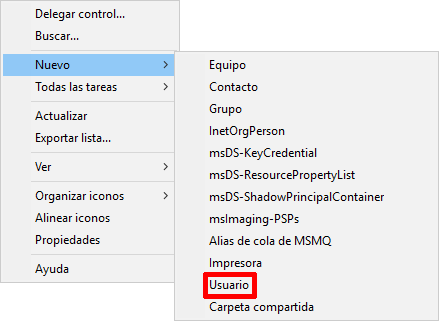
\includegraphics[width=0.5\linewidth]{crear_usuario.png}
    \vspace{-10pt}
\end{center}

Al seleccionar la opción de “Usuario”, nos aparecerá una nueva ventana donde podremos rellenar:

{
    \begin{minipage}{0.6\linewidth}
        \begin{itemize}
            \item \textbf{Nombre de pila}: Nombre del usuario. Este nombre se puede repetir en el servidor.
            \item \textbf{Iniciales}: Formato abreviado del nombre y apellidos
            \item \textbf{Apellidos}: Los apellidos del usuario
            \item \textbf{Nombre completo}: Se autocompleta con lo rellenado en el nombre y los apellidos

        \end{itemize}
    \end{minipage}
    \hfill
    \begin{minipage}{0.37\linewidth}
        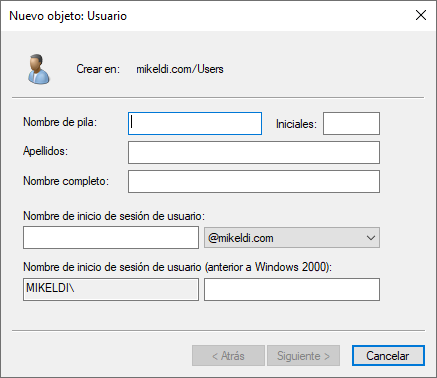
\includegraphics[width=\linewidth]{crear_usuario2.png}
    \end{minipage}
}

\begin{itemize}
    \item \textbf{Nombre de inicio de sesión de usuario}: El nombre que el usuario deberá introducir al encender el ordenador y aparecer la pantalla de inicio de sesión.

    \warnbox{El nombre de inicio de sesión \textbf{no debe repetirse}.}

    \item \textbf{Nombre de inicio de sesión de usuario (Anterior a Windows 2000)}: Debería coincidir con el nombre de inicio de sesión.
\end{itemize}

Tras darle a “Siguiente” nos aparecerá la pantalla donde debemos introducir:

\begin{itemize}
    \item \textbf{Contraseña}: La contraseña que el usuario deberá introducir al iniciar sesión.
    \item \textbf{Confirmar contraseña}: Debe coincidir.
\end{itemize}

Y aparecen cuatro opciones que podemos marcar dependiendo de lo que necesitemos:

{
    \begin{minipage}{0.65\linewidth}
        \begin{itemize}
            \item[\ding{111}] Si permitimos que el usuario pueda cambiar la contraseña la siguiente vez que inicie sesión (al estar creando el usuario, será en el primer inicio de sesión).
            \item[\ding{111}] NO permitir que el usuario pueda cambiar la contraseña. Por lo tanto, en caso de querer modificarla se deberá realizar desde el servidor.

        \end{itemize}
    \end{minipage}
    \hfill
    \begin{minipage}{0.3\linewidth}
        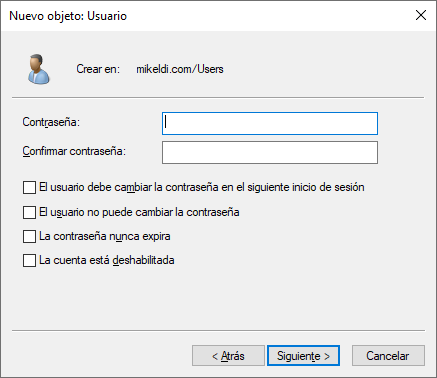
\includegraphics[width=\linewidth]{crear_usuario3.png}
    \end{minipage}
}

\begin{itemize}
    \item[\ding{111}] Que no expire la contraseña, ya que por defecto caducan pasados 42 días.
    \item[\ding{111}] Deshabilitar la cuenta.
\end{itemize}

Al darle a “Siguiente” nos aparecerá el último paso que será el de confirmar la creación del usuario.

\infobox{Todas estas opciones pueden ser modificadas una vez creado el usuario.}


\section{Cuentas de equipo}
Una cuenta de equipo sirve para autenticar a los diferentes equipos que se conectan al dominio, permitiendo o denegando su acceso a los diferentes recursos del dominio. Del mismo modo que con las cuentas de usuario, las cuentas de equipo deben ser únicas en el dominio. Aunque una cuenta de equipo se puede crear de forma manual, lo habitual es que se crean en el momento en el que el equipo se une al dominio.


\chapter{GPO: Directivas de grupos}

Las GPO (\textit{Group Policy Objets}) en castellano conocidas como “Objetos de Políticas de Grupo” (o simplemente directivas de grupo), son los objetos que incluye una serie de directivas (o políticas) que pueden aplicarse de manera centralizada a equipos y usuarios. Cada GPO  establece una configuración del objeto al que afecta. Por ejemplo:

\begin{itemize}
    \item Montar una unidad de red correspondiente
    \item Modificar configuración del firewall
    \item Ocultar el panel de control
    \item …
\end{itemize}

\infobox{Las Directivas de Grupos controlan lo que los usuarios
    y los equipos pueden y no pueden hacer.}

Las GPO se vinculan a nuestra estructura de árbol al nivel al que deseamos configurar. Si vinculamos una GPO en el nombre de nuestro árbol, esta GPO afectará a todo el árbol. Si por el contrario vinculamos nuestra GPO en un nombre de dominio, esa GPO solo afectará a dicho dominio. \textbf{Las GPO se pueden vincular en sitios, dominios y unidades organizativas}. Tal como se puede ver, y pese a su nombre, las GPO \underline{no se pueden asociar a un grupo de usuarios}.

Para crear una GPO, tendremos que ir al “Administrador del Servidor” y en “Herramientas” elegir “Administración de directivas de grupo” (también conocido como \textbf{GPMC.exe}), lo que nos abrirá la siguiente ventana:

\begin{center}
    \vspace{-15pt}
    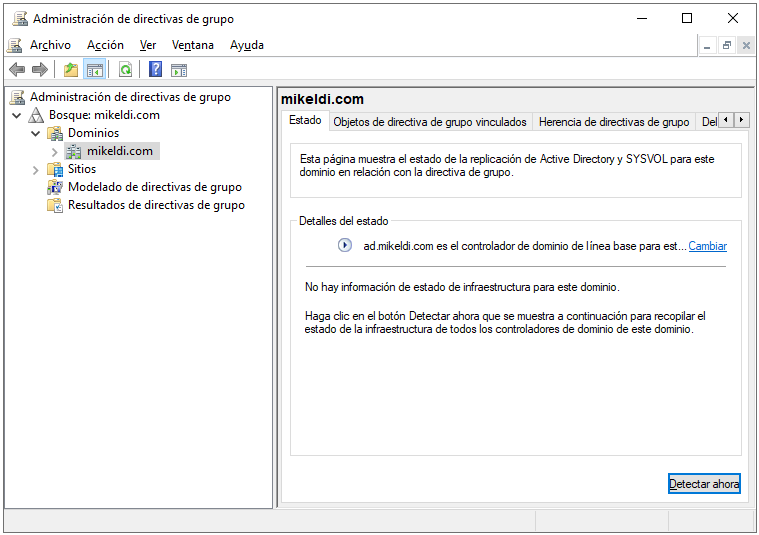
\includegraphics[width=12cm]{gpo_administrar.png}
    \vspace{-25pt}
\end{center}

Las GPOs no se aplican de manera inmediata, ya que el equipo debe reiniciarse o el usuario cerrar sesión. Podemos hacer que desde el equipo un usuario ejecute la orden “\textbf{gpupdate.exe}” y esto forzará la actualización de las GPO, pero requiere de la intervención del usuario. Más adelante vamos a ver cómo forzar la actualización de las GPO de manera remota desde el servidor.


\section{Nivel de aplicación}
Dado que en un bosque podemos tener distintas GPOs que puedan afectar a un mismo objeto, debemos conocer que las directivas se aplican en este orden:

\begin{enumerate}
    \item \textbf{Objeto de directiva de grupo local}: cada equipo tiene exactamente un objeto de directiva de grupo almacenado de forma local. Este objeto controla el procesamiento de las directivas de grupo de equipo y usuario.

    \item \textbf{Sitio}: todos los GPO vinculados al sitio al que pertenece el equipo se procesan a continuación. El procesamiento se efectúa en el orden especificado por el administrador en la ficha \textbf{Objetos de directivas de grupo vinculados} del sitio en la Consola de administración de directivas de grupo (GPMC, Group Policy Management Console). La GPO con el \textbf{orden de vínculos} más bajo es la última en procesarse y, por tanto, tiene la máxima prioridad.

    \item \textbf{Dominio}: el procesamiento de varias GPO vinculadas a un dominio se efectúa en el orden especificado por el administrador, en la ficha \textbf{Objetos de directivas de grupo vinculados} del dominio en GPMC. La GPO con el \textbf{orden de vínculos} más bajo es la última en procesarse y, por tanto, tiene la máxima prioridad.

    \item \textbf{Unidades organizativas}: los GPO vinculados a la unidad organizativa que se encuentra en el nivel más alto de la jerarquía de Active Directory se procesan primero, luego las GPO vinculadas a su unidad organizativa secundaria y así sucesivamente. Por último, se procesan los GPO vinculados a la unidad organizativa que contiene el usuario o el equipo.
\end{enumerate}

\begin{center}
    \vspace{-15pt}
    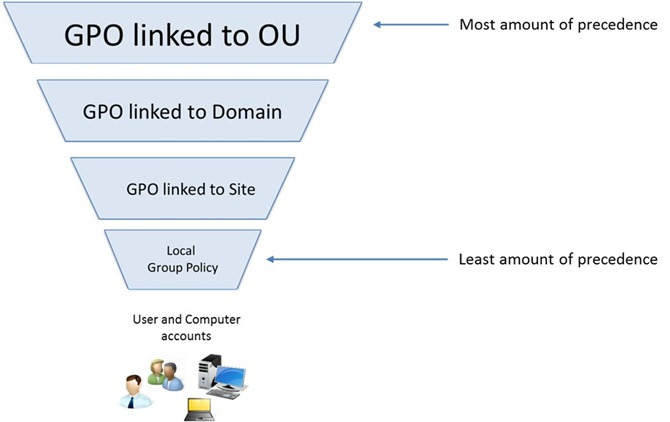
\includegraphics[width=10cm]{gpo.jpg}
    \vspace{-25pt}
\end{center}

La Directiva de Grupo se aplica de manera jerárquica desde el grupo menos restrictivo (Sitio) al grupo más restrictivo (Unidad Organizativa). La Directiva de Grupo también es acumulativa.

El comportamiento respecto a la herencia y prioridad entre GPO en contenedores anidados puede ser refinado mediante los siguientes dos parámetros de configuración:

\begin{itemize}
    \item \textbf{Exigido} (enforced). Este parámetro puede activarse independientemente a cada vínculo de un GPO. Si un vínculo de un GPO a un contenedor tiene este parámetro activado, sus políticas no pueden ser sobrescritas por GPO que se apliquen posteriormente.

    \item \textbf{Bloquear herencia} (de directivas) (Block Policy inheritance). Este parámetro pertenece a los contenedores del Directorio Activo. En particular, si un contenedor tiene este parámetro activado, se desactiva la herencia de las políticas establecidas en contenedores superiores, excepto aquellas que corresponden a GPO vinculados con el parámetro Exigido.
\end{itemize}

Para poder crear o modificar directivas de grupo deberemos ir al asistente de “Administración del Servidor → Herramientas →  Administración de directivas de grupo” o desde el comando \textbf{GPMC.exe}.


\section{Ejemplos prácticos}
A continuación se van a detallar la creación de distintas GPO que podremos utilizar de base para crear otras.

\subsection{Añadir una unidad de red a usuarios}
Es habitual que en una red los usuarios tengan que conectarse a unidades de red. Los usuarios finales no tienen por qué saber cómo conectarse a una unidad de red, y por tanto si les facilitamos el trabajo será más fácil que puedan acceder. En una red con Active Directory podemos indicar que los usuarios tengan distintas unidades de red conectadas en el equipo y con una letra correspondiente en el momento en el que se loguean.

Para el ejemplo se ha creado una Unidad Organizativa llamada “Usuarios” y dentro otra llamada “Sistemas” y dentro tenemos un usuario llamado “sysadmin1” que hemos añadido al grupo “sistemas”:

\begin{center}
    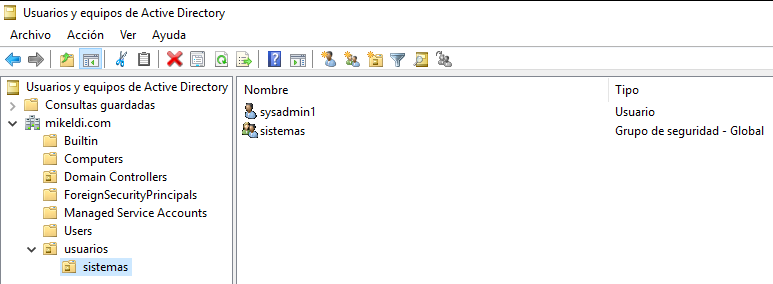
\includegraphics[frame,width=\linewidth]{gpo_1_1.png}
\end{center}


\subsubsection{Crear una carpeta compartida}
Se ha creado una carpeta que hemos dejado en el escritorio del usuario administrador, aunque lo ideal es ponerlo en una ruta más acorde, pero como prueba nos sirve. Esta carpeta va a ser compartida con el grupo “sistemas” que hemos creado previamente:

\begin{center}
    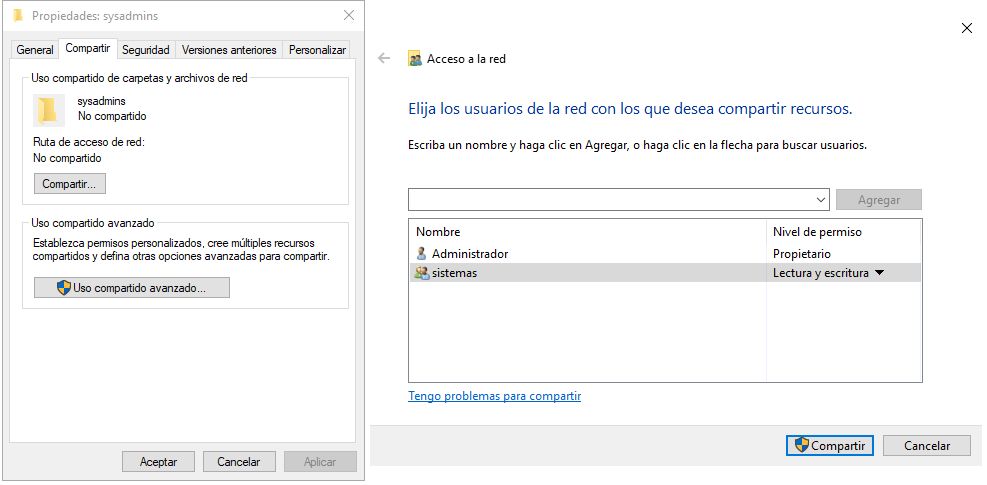
\includegraphics[frame,width=13cm]{gpo_1_2.png}
\end{center}

Tras realizar estos pasos, un usuario que pertenezca al grupo “sistemas” podría conectarse a la carpeta compartida, pero debería conocer la ruta. Vamos a automatizar esto a través de la GPO.

\subsubsection{Crear GPO}
Tal como hemos comentado previamente, la GPO va a permitir que cuando el usuario inicie sesión le aparezca la carpeta compartida como una unidad nueva  con la letra que especifiquemos.
Los pasos para crear la GPO son:

{
    \begin{minipage}{0.6\linewidth}
        \begin{enumerate}
            \item Ir a “Administración de directivas de grupo”
            \item Crear GPO en la unidad organizativa en la que queremos que esté asociado.
            \item Nos aparecerá una nueva ventana en la que podremos introducir un nombre para la GPO que vamos a crear. Este nombre debería darnos información de para qué sirve la GPO, por lo tanto, hay que elegir un nombre representativo, por ejemplo: “montar unidad para sysadmins”
        \end{enumerate}
    \end{minipage}
    \hfill
    \begin{minipage}{0.37\linewidth}
        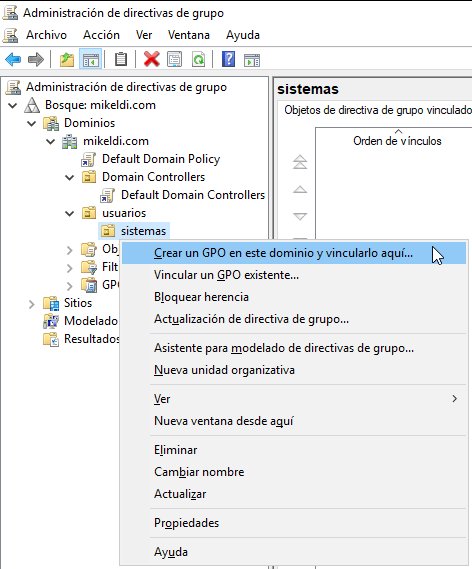
\includegraphics[trim={0 255 0 0},clip,width=\linewidth]{gpo_1_3.png}
    \end{minipage}
}

\begin{enumerate}
    \setcounter{enumi}{3}
    \item Una vez creada, debemos configurar qué acciones queremos que realice. Para ello, haremos click derecho encima de la GPO y le daremos a “Editar”, lo que nos abrirá una nueva ventana con el programa de edición de directivas de grupo, con la directiva que hemos seleccionado.

    \begin{center}
        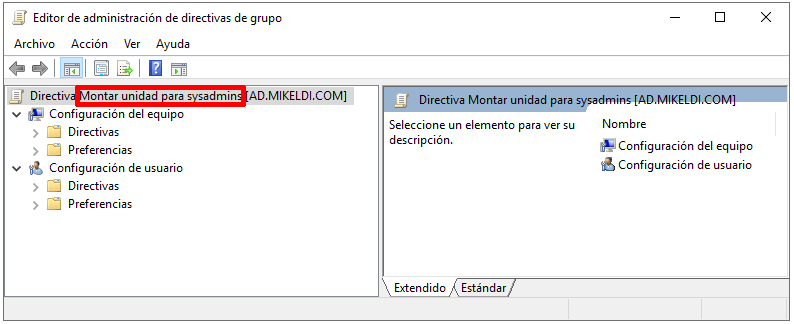
\includegraphics[width=13cm]{gpo_1_4.png}
    \end{center}

    Tal como se puede ver en la imagen, arriba a la izquierda aparece el nombre de la GPO y el servidor en el que está creada. Debajo aparece si va a ser de tipo Configuración del equipo o configuración para usuario.

    \item Vamos a crear una configuración para usuarios, por lo tanto iremos a “\textit{Configuraciones de usuario → Preferencias → Configuración de Windows → Asignaciones de unidades”. Le damos a “Nueva → Unidad asignada}” y deberemos rellenar los datos indicando:
    \begin{enumerate}
        \item Ubicación de los datos
        \item Etiqueta
        \item Letra de unidad
    \end{enumerate}
\end{enumerate}

{
    \begin{minipage}{0.46\linewidth}
        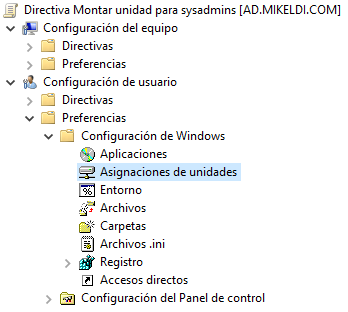
\includegraphics[frame,width=\linewidth]{gpo_1_5.png}
    \end{minipage}
    \hfill
    \begin{minipage}{0.46\linewidth}
        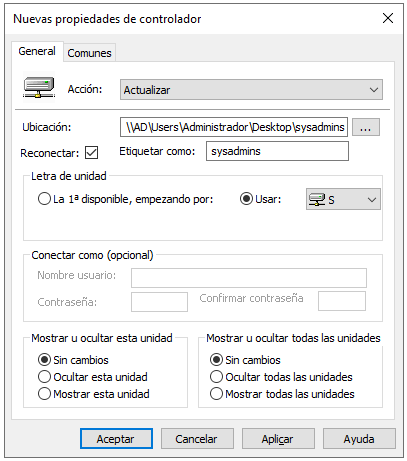
\includegraphics[width=\linewidth]{gpo_1_6.png}
    \end{minipage}
}

Una vez hecho esto, cuando cualquier usuario que esté creado en la Unidad Organizativa “sistemas” inicie sesión, tendrá una unidad compartida en el apartado “Este equipo”:

\begin{center}
    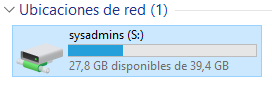
\includegraphics[frame,width=6cm]{gpo_1_7.png}
\end{center}

De esta manera, realizando una única configuración será válida para todos los usuarios que tengamos en esa Unidad Organizativa. El resumen de la GPO es:

\begin{center}
    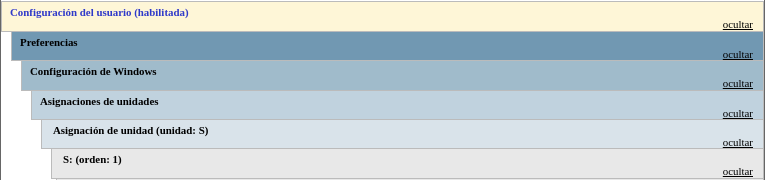
\includegraphics[trim={1 0 0 0},clip,frame,width=14cm]{gpo_1_8.png}
\end{center}


\subsection{Permitir conexiones ping}

Es habitual que los equipos Windows 10 no permitan realizar conexiones del protocolo ICMP (ping) ya que el firewall las rechaza. Por otro lado, para tener controlado los equipos que están encendidos en la red es interesante que esté habilitado.

Dado que ir configurando equipo a equipo el firewall es una tarea tediosa, el realizar la configuración de manera automática mediante una GPO es sencillo y nos permite ver cómo podemos realizar configuraciones que en este caso afectan al equipo y no al usuario.


{
    \begin{minipage}{0.6\linewidth}
        \setlength{\parskip}{1.2em}
        En este caso vamos a crear una GPO que afecte a todos los equipos del dominio, por lo tanto haremos click derecho sobre el dominio y crearemos la GPO en él, poniéndole un nombre como “\textbf{Habilitar ping}”.

        Editamos la GPO y esta vez tenemos que desplegar los menús hasta llegar a: “\textit{Configuración del equipo → Directivas → Configuración de Windows → Configuración de Seguridad → Windows Defender Firewall con seguridad avanzada → Windows Defender Firewall con seguridad avanzada → \textbf{Reglas de entrada}}”.
    \end{minipage}
    \hfill
    \begin{minipage}{0.36\linewidth}
        \vspace{-5pt}
        \hfill
        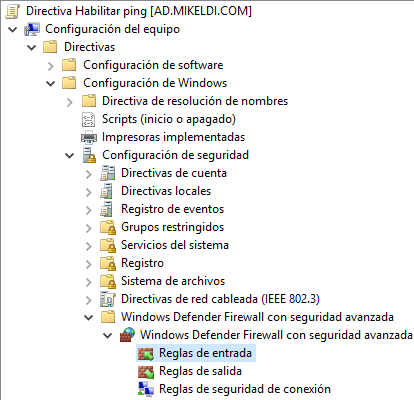
\includegraphics[frame,trim={1 0 0 2},frame,clip,width=\linewidth]{gpo_2_1.png}
    \end{minipage}
}

\vspace{5pt}

Al llegar a este punto, haremos click derecho y le daremos a “Nueva regla” y vamos a seguir el asistente de creación de una nueva regla personalizada que permita el protocolo ICMPv4 de entrada desde cualquier equipo.

\begin{center}
    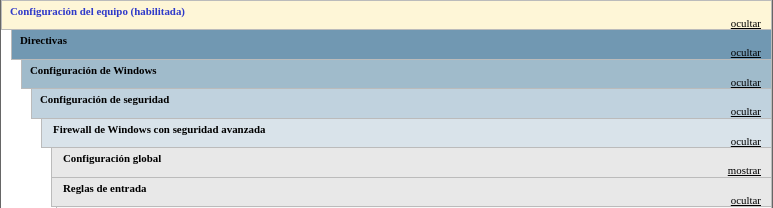
\includegraphics[trim={1 0 0 0},clip,frame,width=14cm]{gpo_2_2.png}
\end{center}

Una vez creada la GPO se aplicará cuando los equipos reinicien. Para evitar tener que reiniciar al crear nuevas GPO, vamos a crear la siguiente GPO que permitirá la administración del equipo de manera remota.


\subsection{Administración remota de equipos}
Tal como hemos dicho anteriormente, las GPOs no se aplican de manera inmediata, y dependiendo de si son de equipo o de usuario se deberá reiniciar o cerrar sesión.

Para poder actualizar las GPOs de manera remota  vamos a crear una GPO que va a permitir la conexión desde el servidor a los equipos y que permitirá recibir la orden de actualizar las GPOs entre otras cosas. Para tener ordenados los equipos, vamos a crear una “OU” llamada “equipos” y dentro de ella otras “OU” para cada departamento que queramos. Los equipos que tengamos en la red los deberemos ordenar en estas Unidades Organizativas creadas, y de esta manera podremos mandar la actualización a los equipos que nos interese.

Vamos a crear una nueva GPO llamada “Permitir actualizar GPOs desde servidor” y la vamos a crear en la “OU” de “equipos”.

La ruta para crear es: “\textit{Configuración del equipo → Plantillas Administrativas → Red → Conexiones de red → Firewall De Windows Defender → Perfil de dominio → \textbf{Firewall de Windows Defender: permitir excepción de administración remota entrante}}”, la cual habilitaremos pero sólo permitiendo la IP de nuestro servidor. El resumen de la GPO sería el que aparece en la imagen:

\begin{center}
    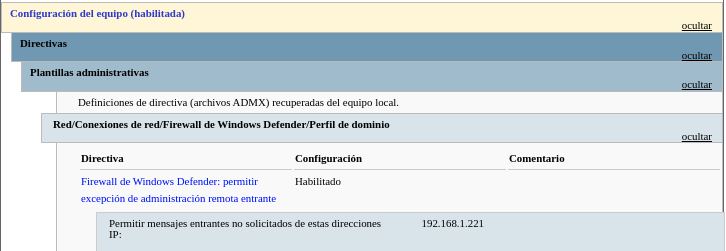
\includegraphics[trim={1 0 0 2},clip,frame,width=14cm]{gpo_3_1.png}
\end{center}

Para aplicar esta GPO el equipo remoto deberá reiniciarse. A partir de este momento, cuando ya se haya aplicado la GPO podremos forzar la actualización de las GPO desde el servidor desde el propio “Administrador de directivas de grupo”, haciendo click derecho sobre la OU donde están los equipos que nos interesa y dando a “Actualización de directiva de grupo”

{
    \begin{minipage}{0.48\linewidth}
        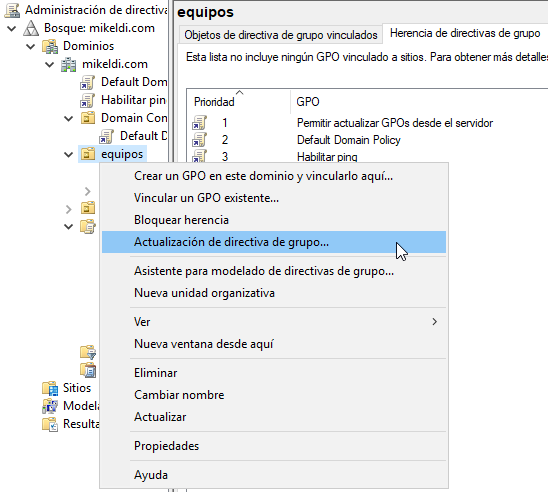
\includegraphics[frame,width=\linewidth]{gpo_3_2.png}
    \end{minipage}
    \hfill
    \begin{minipage}{0.48\linewidth}
        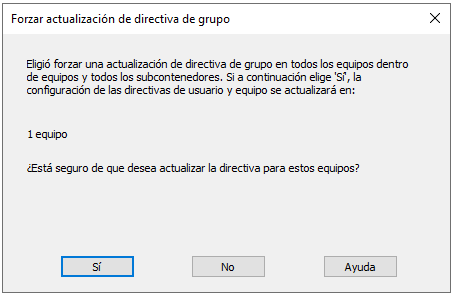
\includegraphics[width=\linewidth]{gpo_3_3.png}
    \end{minipage}
}

Tras confirmar que queremos actualizar las directivas para el número de equipos que estén en esa Unidad Organizativa, nos aparecerá un mensaje de confirmación de que el proceso se ha realizado de manera correcta:

\begin{center}
    \includegraphics[width=10cm]{gpo_3_4.png}
\end{center}

Debemos fijarnos que en la columna central no aparece ningún código de error. Este proceso hará que las GPOs se recarguen en una tarea que se va a ejecutar en el equipo remoto en los \textbf{próximos 10 minutos}. Si queremos que sea inmediato podemos forzar la actualización mediante un comando en powershell.

También podremos administrar los equipos desde el programa de “Usuarios y equipos de Active Directory”, eligiendo el equipo que queramos y darle a “Administrar”:

\begin{center}
    \includegraphics[frame,width=10cm]{gpo_3_5.png}
\end{center}

Lo que nos abrirá el asistente de administración remota:

\begin{center}
    \includegraphics[width=14cm]{gpo_3_6.png}
\end{center}

Y desde aquí podremos realizar parte de la administración remota del equipo.


\subsection{Habilitar acceso al escritorio remoto}
En una red no siempre tenemos acceso a los equipos de los usuarios, por encontrarse en otras sedes, oficinas o situaciones geográficas. Es por esto por lo que el poder acceder a los equipos de los usuarios puede suponer una ventaja administrativa a nivel global.

Para ello, podemos crear una GPO para que los equipos que están en nuestro Active Directory se les active el acceso remoto para poder así conectarnos a ellos.

Los pasos a dar cuando creamos la GPO son:

\begin{enumerate}
    \item \textbf{Habilitar escritorio remoto}: “\textit{Configuración del equipo  →  Directivas  →  Plantillas administrativas \hfill →   Componentes de Windows → Servicios de Escritorio remoto → Host de sesión de Escritorio remoto → Conexiones → Permitir que los usuarios se conecten de forma remota mediante Servicios de Escritorio remoto}”

    \begin{center}
        \includegraphics[trim={2 0 0 0},clip,frame,width=14cm]{gpo_4_1.png}
    \end{center}

    \item Habilitar el acceso en el firewall al puerto necesario (RDP, que es 3389). Existe una plantilla para ello en: “\textit{Configuración del equipo → Directivas → Plantillas administrativas → Red → Conexiones de Red → Firewall de Windows Defender → Perfil de dominio}” y aceptar conexiones desde la IP del servidor.

    \begin{center}
        \includegraphics[trim={1 0 0 0},clip,frame,width=14cm]{gpo_4_2.png}
    \end{center}
\end{enumerate}

Si queremos que cualquier otro usuario que no sea el Administrador pueda realizar conexiones mediante escritorio remoto, tendremos que meterlo en el grupo “Usuarios de escritorio remoto” que está dentro de “Builtin”, ya que es un grupo que se ha creado durante la instalación de Active Directory.

\begin{center}
    \includegraphics[trim={1 0 0 0},clip,frame,width=14cm]{gpo_4_3.png}
\end{center}



\chapter{Alta Disponibilidad en Active Directory}
Cuando hablamos de Alta Disponibilidad hacemos referencia al diseño de una infraestructura de servicios y de servidores en la que no existe un único punto de fallo. Hasta ahora, nuestro dominio está controlado por un único servidor que realiza la función de Controlador de Dominio, por lo que en caso de catástrofe, perderíamos la posibilidad de configurar el dominio, añadir nuevos usuarios…

Para evitar ese único punto de fallo, es conveniente realizar la instalación de un nuevo servidor y configurarlo para que actúe como servidor réplica del controlador de dominio principal.


\section{Instalación del  servidor réplica}
La instalación del servidor réplica será igual que la del primer controlador de dominio, tal como hemos visto anteriormente. Lógicamente nos aseguraremos que el servidor cuente con otro nombre y otra dirección IP que no coincida con el servidor principal.

También realizaremos la instalación del rol de “\textbf{Servicios de dominio de Active Directory}” ya que lo vamos a necesitar más adelante.

\section{Meter servidor en el dominio actual}
El primer paso es meter el nuevo servidor como un equipo más en el dominio del que queremos ser réplica. Los pasos a dar son los vistos anteriormente para un equipo Windows 10.

Tras realizar el reinicio correspondiente, vamos a promocionar el nuevo servidor para que actúe como servidor réplica.


\section{Configurar nuevo Active Directory como servidor réplica}
Para promocionar el nuevo servidor Active Directory para que actúe como servidor réplica del dominio debemos ir al “Administrador del servidor” y pinchar sobre el aviso para promocionarlo, tal como hicimos en el servidor principal.

Al darle a promocionar, nos aparecerá en la nueva ventana la opción de “\textbf{Agregar un controlador de dominio a un dominio existente}” seleccionada, con el dominio correspondiente al que nos hemos metido previamente. Le daremos a “Cambiar” y meteremos las credenciales de Administrador del dominio. De esta manera, tendremos la ventana tal como aparece en la siguiente imagen y podremos dar a “Siguiente”.


{
    \begin{minipage}{0.48\linewidth}
        \includegraphics[width=\linewidth]{HA_active_directory_1.png}
    \end{minipage}
    \hfill
    \begin{minipage}{0.48\linewidth}
        \includegraphics[width=\linewidth]{HA_active_directory_2.png}
    \end{minipage}
    \vspace{1em}
}

En este paso podremos elegir si queremos que nuestro servidor sea configurado en modo “sólo lectura” (por lo que realizará la réplica de datos, pero no podremos crear nada en él) y nos preguntará por la contraseña DSRM para este servidor. Una vez introducida, continuamos hasta llegar al siguiente paso.

{
    \begin{minipage}{0.48\linewidth}
        \setlength{\parskip}{1.2em}
        En este paso nos permitirá realizar las opciones del DNS que necesitemos. En nuestro caso, vamos a continuar al siguiente paso sin realizar modificaciones en este apartado, por lo que llegaremos a las “opciones adicionales”:
    \end{minipage}
    \hfill
    \begin{minipage}{0.48\linewidth}
        \includegraphics[width=\linewidth]{HA_active_directory_3.png}
    \end{minipage}
}

\vspace{5pt}

Tal como se puede ver en la captura de pantalla, podremos elegir desde qué servidor queremos realizar la réplica de los datos. En nuestra infraestructura sólo tenemos otro servidor, por lo que no importa si seleccionamos el servidor o la opción “Cualquier controlador de dominio”. Esta opción es útil cuando ya tengamos previamente dos o más servidores, ya que por conectividad nos puede interesar que realice la réplica desde uno en concreto.

Los siguientes pasos los dejaremos tal como están hasta realizar la instalación y que el servidor se reinicie.

\section{Comprobación del funcionamiento de la réplica}
Una vez reiniciado el servidor réplica, veremos que al iniciar sesión nos aparecerán los grupos, usuarios y GPOs que teníamos en el servidor principal. Si vamos al gestor de “Usuarios y equipos de Active Directory” veremos que el nuevo servidor aparece dentro del apartado “Domain Controller”:

\begin{center}
    \vspace{-10pt}
    \includegraphics[width=0.8\linewidth]{HA_active_directory_4.png}
\end{center}

Si creamos un nuevo usuario en cualquiera de los dos servidores, comprobaremos cómo en el otro servidor nos aparece también. De ser así, la réplica está funcionando de manera correcta.

\section{Configuración final}
Para dejar nuestra configuración final correcta debemos de realizar una pequeña modificación en los DNS de los servidores y también en los clientes.

El cambio de configuración es que los servidores tienen que tener al otro servidor como DNS principal, y a sí mismos como DNS secundarios. Es decir, configuración cruzada:

\begin{center}
    \vspace{-10pt}
    \includegraphics[width=0.5\linewidth]{HA_active_directory_5.png}
\end{center}

Tal como se puede ver en la imagen, contamos con dos servidores para el dominio “mikeldi.com”, ambos se replican entre sí y cada uno tiene como DNS principal al otro servidor.

Por otro lado, en lo referente a los equipos, la configuración debe ser igual: deben de tener como DNS principal uno de los servidores y como DNS secundario el otro . De esta manera, si el servidor que actúa como DNS principal cae, los equipos realizarán las peticiones al otro servidor. Esta modificación de DNS lo habitual es que se realice mediante el servidor DHCP en lugar de ir equipo por equipo (ya que es una tarea tediosa y fácilmente automatizable).


\part{GNU/Linux como servidor de red}
\graphicspath{{img/linux/}}
\chapter{Introducción a GNU/Linux}
\section{Un poco de historia}
Para conocer cómo nació el movimiento GNU y el kernel Linux debemos conocer un poco de historia de la informática y cómo evolucionó en los primeros años.

\subsection{El nacimiento de Unix}

\begin{description}
\item[1964-1969]Los laboratorios \textbf{Bell} empiezan un proyecto con el \textbf{MIT} (Instituto Tecnológico de Massachusetts) y \textbf{General Electric} para desarrollar un sistema de \textbf{tiempo compartido} (“time-sharing computing”): se llamaría \textbf{Multics} (Multiplexed Information and Computing Service).

Hasta este momento, los sistemas utilizados eran de un único proceso, la CPU no era compartida por múltiples procesos sino que se ejecutaba por lotes (se les mandaba los procesos a ejecutar y se ejecutaban en orden).

Multics obtuvo licencia libre en el 2007. En Diciembre del 2016 salió la última versión 12.6f.

\itemimage{1969}{r}{0.33}
  {/Ken_Thompson_and_Dennis_Ritchie--1973.jpg}
  {\href{https://en.wikipedia.org/wiki/Ken_Thompson}{Ken y Dennis. Origen: Wikipedia}}
  {
  Uno de los desarrolladores de Multics, \href{https://en.wikipedia.org/wiki/Ken_Thompson}{Ken Thompson}, decidió escribir su propio sistema operativo. Ken Thompson es conocido también por crear el lenguaje de programación \textbf{B}, el sistema de codificación de caracteres UTF-8 y el lenguaje de programación Go, entre otras cosas.

A Ken Thompson se le une \href{https://en.wikipedia.org/wiki/Dennis_Ritchie}{Dennis Ritchie} y otros, y empiezan a programar un sistema de ficheros jerárquico, el concepto de procesos de computación, ficheros de dispositivos, un intérprete de comandos, … El resultado de lo programado era más pequeño y simple que Multics, lo que se convertiría en Unix. En Agosto ya tendrían el sistema operativo, se auto-gestiona,  tenía un assembler, un editor y una shell de comandos.

Dennis Ritchie es conocido también por crear junto con Ken el lenguaje de programación \textbf{C} (aparece por primera vez en 1972).
}


\item[1970]En ese momento el nuevo sistema operativo se llamaba \textbf{Unics} (\textit{Uniplexed Information and Computing Service}, un juego de palabras en contraposición a  Multics). No tenían todavía dinero de la organización en el desarrollo (era desarrollado por los programadores) y tampoco era multitarea todavía.

A finales de año el sistema ya era conocido como \textbf{UNIX}, y se había portado a la máquina PDP-11.

\textbf{Las primeras versiones de Unix incluían el código fuente} para que las universidades lo pudiesen modificar y así poder extenderlo a sus necesida des.


\item[1971]El sistema se empieza a hacer complejo y como querían que más usuarios lo usasen, crean el sistema de manuales que es utilizado hoy en día (mediante el comando \textbf{"man"}).

\begin{center}
  \includegraphics[width=0.8\linewidth]{/Ken_Thompson_(sitting)_and_Dennis_Ritchie_at_PDP-11_(2876612463).jpg}
  \vspace{-10pt}\captionof{figure}{\href{https://en.wikipedia.org/wiki/Ken_Thompson}{Dennis Ritchie y Ken Thompson trabajando en un PDP-11. Origen: Wikipedia}}\vspace{-13pt}
\end{center}


\item[1973]La versión 4 del sistema es reescrita completamente en C. Hasta este momento el sistema había estado escrito en ensamblador, por lo que no era portable entre distintos tipos de máquinas, aunque la primera versión portada a otra plataforma fue en 1978. Se cree que había “más de 20” instalaciones del sistema.

\item[1974]La versión 5 se licencia para ser utilizada en \textbf{instituciones educativas}.

\item[1975]La versión 6 se licencia para poder ser utilizadas por empresas por \$20.000 de la época.

\item[1977]La universidad de Berkeley lanza su primera versión de Unix bajo la Berkeley Software Distribution (BSD).

\item[1979]Con la salida de Unix v7, se comienza a portar a los distintos ``microordenadores'' de la época y a los distintos microprocesadores (Motorola 68000, Intel 8086, … ).

\item[1980]Microsoft anuncia su primer Unix para microcomputadoras de 16 bits (Xenix).
\end{description}

\subsection{El nacimiento de GNU (GNU's Not Unix}
\begin{description}

\item[1971]\href{https://en.wikipedia.org/wiki/Richard_Stallman}{Richard Stallman} comienza su carrera en el MIT en el laboratorio de inteligencia artificial.

Es conocido no sólo por el movimiento GNU, si no también por crear GCC y Emacs entre otra gran cantidad de software.

En esa época el software se distribuía de manera abierta para poder ser modificado. Lo habitual era realizar modificaciones para mejorar el software y distribuirlo entre compañeros y universidades.

\itemimage{1982}{r}{0.25}
  {/Richard_Stallman_2016_Talk_in_Madrid_06.jpg}
  {\href{https://commons.wikimedia.org/wiki/File:Richard_Stallman_2016_Talk_in_Madrid_06.jpg}{Richard Stallman: Wikimedia}}
  {
Richard Stallman quiere modificar el firmware de unas impresoras y el fabricante le pide que firme un acuerdo de no divulgación si le enseñan el código. Esto hace que Stallman se enfurezca y es cuando decide que la situación actual debe cambiar y volver al sistema de intercambio de software anterior.

\item[1983] Se anuncia el nacimiento del proyecto \textbf{GNU}, cuya finalidad es la de construir un sistema operativo completamente libre, compatible con Unix. La idea es dar a los usuarios la libertad y el control de sus ordenadores.

\item[1985] Se lanza el \href{https://www.gnu.org/gnu/manifesto.es.html}{manifiesto GNU}, y ya cuenta con un editor de texto (Emacs), compilador de C, una shell, varias utilidades … El núcleo inicial todavía no es funcional.
}


\item[1986]
Richard Stallman escribe y publica la definición de lo que es Free Software (Software Libre) a través de la \href{https://es.wikipedia.org/wiki/Free_Software_Foundation}{Free Software Foundation}.

\begin{tcolorbox}[title=Aclarando la palabra “free”:,sidebyside,righthand width=0.12\linewidth]

\textbf{The word “free” in our name does not refer to price; it refers to freedom.}

La palabra “free” no se refiere a gratis, si no que se refiere a libertad.

\tcblower
\includegraphics[width=\linewidth]{/gnu.png}
\end{tcolorbox}

Más adelante veremos a qué se refiere sobre libertad en el software.

\end{description}

\subsection{El nacimiento de Minix}
\begin{description}
\item[1987]Andrew S. Tanenbaum crea  Minix como propósito educativo y para enseñar cómo funciona un sistema operativo.

\item[1991]Sale la versión 1.5 de Minix y es portada a distintas arquitecturas (IBM, Motorola 68000, Amiga, Apple Macintosh, …).

\item[1992]Debate con Linus Torvalds sobre la arquitectura del kernel Linux (núcleo monolítico) en lugar de usar un micronúcleo.

\end{description}


\subsection{El nacimiento de Linux}
\begin{description}

\item[1991] Un estudiante en la universidad de Helsinki, \href{https://en.wikipedia.org/wiki/Linus_Torvalds}{Linus Torvalds}, comienza un proyecto personal escrito para su nuevo ordenador, un PC con procesador 80386.

El desarrollo comienza bajo \textbf{Minix}, usando el compilador \textbf{GCC} del movimiento GNU (GCC = GNU Compiler Collection).

El proyecto termina convirtiéndose en un kernel de un sistema operativo y escribió al grupo de noticias de Minix diciendo:

\begin{tcolorbox}[title=Email de Linus Torvalds presentando Linux,sidebyside,righthand width=0.30\linewidth]
  “Hola a todos los que estáis ahí fuera usando minix.\\


  Estoy haciendo un sistema operativo (libre), (solamente por aficion, no será grande ni profesional como el GNU) para clones 386(486) AT.

  ...

  PD. Sí – está libre de cualquier código de minix, y tiene un sistema de ficheros multi-hilo. NO es portable (usa el cambio de tareas del 386 etc), y probablemente nunca soporte otra cosa que no sean los discos duros AT, porque es todo lo que tengo :-(. ”
  \tcblower
  \includegraphics[width=\linewidth]{/Linus_Torvalds.jpeg}
  \vspace{-30pt}\captionof{figure}{\href{https://en.wikipedia.org/wiki/Linus_Torvalds}{Linus torvalds. Origen: Wikipedia}}
\end{tcolorbox}


\item[1992] Originalmente la licencia de Linux era propia e impedía el uso comercial de Linux. En la versión 0.99 esto cambia y se cambia a la licencia GNU Public License (\textbf{GPL}).

\item[1993] El proyecto cuenta con más de 100 desarrolladores. El kernel se adapta al entorno del proyecto GNU. Nace la distribución \textbf{Debian} (una de las más importantes a día de hoy)

\begin{center}
  \includegraphics[width=0.5\linewidth]{/debian-logo.jpg}
  \vspace{-10pt}\captionof{figure}{\href{https://www.debian.org}{Debian}}
\end{center}

\item[1994] Se libera la versión 1.0. El proyecto XFree86 se une y Linux consigue interfaz gráfico. Nacen las primeras distribuciones comerciales \textbf{Red Hat} y \textbf{Suse}.

\item[1998] Empresas como \textbf{IBM}, \textbf{Compaq} y \textbf{Oracle} anuncian que apoyan a Linux. Nace el interfaz gráfico \textbf{KDE}.

\item[1999] Nace el interfaz gráfico \textbf{GNOME} como reemplazo a KDE, ya que KDE hacía uso de una librería propietaria en aquel momento (QT).

\item[2001] Steve Ballmer (CEO de Microsoft) dice: \textbf{“Linux es un cáncer”}.

\item[2002] Se libera OpenOffice (originalmente suite ofimática de Sun Microsystems). Nace Mozilla (hoy día:  Firefox).

\item[2003] IBM lanza un anuncio para la Linux Foundation: \href{https://www.youtube.com/watch?v=x7ozaFbqg00}{https://www.youtube.com/watch?v=x7ozaFbqg00}

\item[2004] Nace \textbf{Ubuntu} (basándose en Debian) y Steve Ballmer (CEO de Microsoft) dice que Linux infringe muchas de sus patentes.

\item[2008] Nace \textbf{\href{https://es.wikipedia.org/wiki/Android}{Android}}, sistema operativo con kernel Linux. Actualmente es el sistema operativo de móviles que más terminales tiene.

\item[2009] Red Hat iguala a Sun Microsystem en capitalización bursátil (un gran logro simbólico).

\item[2014] Satya Nadella (CEO de Microsoft) muestra en una presentación la siguiente transparencia:

\begin{center}
  \includegraphics[width=0.5\linewidth]{/Microsoft_Linux.jpg}
  \vspace{-10pt}\captionof{figure}{\href{https://commons.wikimedia.org/wiki/File:Microsoft_Linux.jpg}{Origen: Wikipedia}}
\end{center}


\item[2016]
Microsoft anuncia \href{https://es.wikipedia.org/wiki/Windows_Subsystem_for_Linux}{WSL} (\textit{Windows Subsystem for Linux}) y se puede instalar en Windows 10 y Windows Server 2019. Permite correr ejecutables de Linux nativamente.

\end{description}

\subsection{Cronograma de sistemas Unix}
En el siguiente cronograma se puede ver la línea temporal de los sistemas Unix:

\begin{center}
  \includegraphics[width=0.7\linewidth]{/Evolución_UNIX.png}
  \vspace{-10pt}\captionof{figure}{\href{https://commons.wikimedia.org/wiki/File:Evolución_UNIX.png}{Origen: Wikipedia}}
\end{center}

\section{Resumen}
Linux es conocido como un sistema operativo libre pero el nombre de Linux se  centra única y exclusivamente en el \textbf{kernel} (o \textbf{núcleo}) del sistema operativo.

El sistema operativo completo debería llamarse \textbf{GNU/Linux}, ya que el kernel es una “pequeña” parte (aunque muy importante) dentro de todo el sistema operativo. El resto de herramientas utilizadas en el sistema operativo pertenecen al proyecto GNU.


\chapter{Licencias Libres}
\section{Software Libre}

En 1986 Richard Stallman saca a la luz la definición de lo que es Free Software (Software Libre) a través de la \href{https://es.wikipedia.org/wiki/Free_Software_Foundation}{Free Software Foundation}:

\begin{tcolorbox}[title=Aclarando la palabra “free”:,sidebyside,righthand width=0.12\linewidth]

    \textbf{The word “free” in our name does not refer to price; it refers to freedom.}

    La palabra “free” no se refiere a gratis, si no que se refiere a libertad.

    \tcblower
    \includegraphics[width=\linewidth]{/gnu.png}
\end{tcolorbox}


Las libertad en el software se refiere a:
\begin{tcolorbox}[title=Libertades del Software Libre:]
    \begin{enumerate}
        \setcounter{enumi}{-1}
        \item La libertad de ejecutar el programa, para cualquier propósito .

        \item La libertad de estudiar cómo trabaja el programa, y cambiarlo para que haga lo que usted quiera. El acceso al código fuente es una condición necesaria para ello.

        \item La libertad de redistribuir copias para que pueda ayudar al prójimo.

        \item La libertad de mejorar el programa y publicar sus mejoras, y versiones modificadas en general, para que se beneficie toda la comunidad. El acceso al código fuente es una condición necesaria.
    \end{enumerate}
\end{tcolorbox}

El movimiento del Free Software es un movimiento que tiene que ver más con la filosofía y la ética que con la tecnología en sí misma.


\subsection{Copyleft y GNU Public License (GPL)}
Es una práctica legal que consiste en el ejercicio del derecho de autor (copyright en inglés) con el objetivo de propiciar el libre uso y distribución de una obra, exigiendo que los concesionarios preserven las mismas libertades al distribuir sus copias y derivados (\href{https://es.wikipedia.org/wiki/Copyleft}{Wikipedia}).

\begin{center}
  \includegraphics[width=\linewidth]{Mapa_conceptual_del_software_libre.png}
  \vspace{-30pt}\captionof{figure}{\href{https://commons.wikimedia.org/wiki/File:Mapa_conceptual_del_software_libre.png}{Mapa conceptual del Software Libre: Wikipedia}}\vspace{-20pt}
\end{center}

Con esto nació la licencia GNU GPL, la cual permite al usuario final la libertad de usar, estudiar, compartir y modificar el software recibido. Tiene que quedar claro que un programa comercial puede ser Software Libre.

\subsection{Diferencias con el Open Source}
Los programas Open Source son aquellos que podemos ver el código fuente pero esto no quiere decir que podamos modificarlo o adaptarlo a nuestras necesidades.

El Open Source es menos restrictivo que el Software Libre y se puede decir que todo Software Libre es Open Source, pero no todo Open Source tiene por qué ser libre.


\section{Licencias libres más conocidas}
Un listado de las licencias libres más utilizadas:

\begin{itemize}
    \item \href{https://es.wikipedia.org/wiki/GNU_General_Public_License}{GNU GPL}
    \item \href{https://es.wikipedia.org/wiki/Licencia_BSD}{BSD}
    \item \href{https://es.wikipedia.org/wiki/Licencia_MIT}{MIT}
    \item \href{https://es.wikipedia.org/wiki/Apache_License}{Licencia Apache}
    \item \href{https://es.wikipedia.org/wiki/Licencia_PHP}{Licencia PHP}
    \item \href{https://es.wikipedia.org/wiki/Licencias_Creative_Commons}{Creative Commons} (no todas las versiones). Más utilizadas en contenido multimedia.
\end{itemize}


\chapter{Sistema de ficheros en GNU/Linux}
El sistema de ficheros en GNU/Linux, al igual que en Unix, es jerárquico, comenzando en la raíz denominada “/”. Partiendo de esta raíz, el resto del sistema de ficheros nace en forma de ramificaciones generando lo que se denominan “rutas de ficheros”, que es el camino completo para llegar al mismo.

\section{Filesystem Hierarchy Standard}
Debido a que en GNU/Linux todo se representa como ficheros (discos, dispositivos, programas, … ) es necesario que exista un orden a la hora de ser almacenados. Con esa intención nace en 1993 el estándar de la jerarquía de ficheros de Linux, enfocado a reestructurar los archivos. Posteriormente se unieron otros derivados de UNIX (la comunidad de desarrollo de BSD) por lo que terminó adoptando el nombre FHS.

Aún siendo un estándar, no todas las distribuciones lo siguen al pie de la letra, y otros Unix, como MacOS, tienen sus propias rutas especiales.


\section{Directorios importantes}
A continuación se exponen los directorios más importantes del sistema junto con la descripción del contenido que deben de tener:
\begin{itemize}

    \item \textbf{/boot/}: archivos de arranque del kernel, normalmente junto con la configuración utilizada para compilarlos.
    \item \textbf{/dev/}: contiene archivos especiales de bloque que representan los dispositivos del hardware que está corriendo el sistema operativo
    \item \textbf{/etc/}: contiene los archivos de configuración del servidor y de los servicios que corren en él. Está subdividido en directorios por servicios o configuraciones.
    \item \textbf{/home/}: los directorios de trabajo de los usuarios normales del sistema
    \item \textbf{/lib/}: librerías que hacen funcionar a los programas
    \item \textbf{/root/}: es la home del usuario root
    \item \textbf{/var/}: archivos variables del sistema
    \begin{itemize}
      \item \textbf{/var/lib/}: aquí se suelen guardar los ficheros de los programas que “crecen”: bases de datos, ficheros caché…
      \item \textbf{/var/log/}: los logs del sistema
    \end{itemize}
\end{itemize}

Junto a todos estos directorios, se ha separado los lugares en los que van los binarios, o ejecutables de los programas. Lo habitual es que se encuentren en estas rutas:

\begin{itemize}
    \item \textbf{/bin/}: aplicaciones esenciales del sistema
    \item \textbf{/sbin/}: aplicaciones que en principio sólo debería ejecutar el usuario root o programas de administración del sistema
    \item \textbf{/usr/bin/}: ejecutables de usuario
    \item \textbf{/usr/sbin/}: ejecutables de superusuario
\end{itemize}
Aunque las rutas de los ejecutables denotan quién debería ejecutar el programa, en la vida real no tiene por qué ser una limitación.

\section{Dispositivos de almacenamiento y discos duros}
En sistemas operativos Windows es habitual que cada partición cuente con una letra para acceder a ella, al igual que ocurre cuando introducimos un dispositivo de almacenamiento externo (un pendrive).

Tal como se ha comentado, en sistemas Unix el sistema de ficheros es una jerarquía, y por tanto todo dispositivo de almacenamiento nuevo deberá estar montado bajo la raíz “/”. Hoy día, en distribuciones con escritorio, al introducir un pendrive éste es auto-montado (es accesible) desde la ruta \textbf{/media/}, donde aparecerán tantos directorios como discos hayamos conectado.

\subsection{Almacenamiento permanente}
Si queremos que un disco duro nuevo sea permanente en nuestro sistema, podremos montarlo en cualquier lugar de la estructura jerárquica. Debido a este sistema, el usuario final no se tendrá que preocupar en almacenar los ficheros en una ruta distinta, si no que será el administrador el que haya hecho que esa ruta ahora pertenezca a un disco duro nuevo.

Imaginemos que el sistema operativo se ha instalado en un disco duro pequeño de 32Gb de espacio y se está llenando, y el directorio que más ocupa es el directorio de los usuarios. Podremos añadir al servidor un nuevo disco duro montado en /home y por tanto a partir de ahora los datos guardados en /home estarán en un nuevo disco duro más grande.

\begin{mycode}{Ejemplo de discos en un sistema con ``lsblk''`}{console}{}
root@vega:~# lsblk
NAME                       MAJ:MIN RM   SIZE RO TYPE MOUNTPOINTS
sda                          8:0    0   1,8T  0 disk
└─sda1                       8:1    0   1,8T  0 part /home/backup

sdb                          8:16   0   3,6T  0 disk
└─sdb1                       8:17   0   3,6T  0 part /home/disco4tb
sdc                          8:32   0 447,1G  0 disk
├─sdc1                       8:33   0   529M  0 part
├─sdc2                       8:34   0   100M  0 part
├─sdc3                       8:35   0    16M  0 part
└─sdc4                       8:36   0 446,5G  0 part
nvme0n1                    259:0    0 931,5G  0 disk
├─nvme0n1p1                259:1    0   512M  0 part
└─nvme0n1p2                259:2    0   800G  0 part /home
nvme1n1                    259:3    0 931,5G  0 disk
├─nvme1n1p1                259:4    0   512M  0 part /boot/efi
├─nvme1n1p2                259:5    0    90G  0 part /
├─nvme1n1p3                259:6    0   300G  0 part
│ ├─VMs-ubuntu--20.04--so1 254:0    0    10G  0 lvm
│ ├─VMs-manjaro            254:2    0    20G  0 lvm
│ └─VMs-win10              254:3    0    35G  0 lvm
└─nvme1n1p4                259:7    0 156,2G  0 part
\end{mycode}


\chapter{Gestión de usuarios locales en GNU/Linux}
En las distribuciones GNU/Linux lo habitual suele ser que existan al menos dos usuarios tras una instalación:

\begin{itemize}
    \item \textbf{root}: usuario administrador o súper usuario.
    \item \textbf{usuario no-privilegiado}: durante la instalación de la distribución nos suele preguntar para crear un usuario del sistema, que no tendrá privilegios.
\end{itemize}


El usuario root, como se ha dicho previamente, es el administrador del sistema, tiene permisos para realizar cualquier tarea dentro de nuestro sistema: instalar paquetes, desinstalarlos, modificar cualquier fichero, realizar formateos... Por lo tanto, el \textbf{realizar tareas como usuario root puede ser peligroso si cometemos algún fallo}.

Las buenas prácticas nos dicen que las tareas cotidianas del sistema deberíamos realizarlas como usuario normal y \textbf{sólo convertirnos en root cuando sea estrictamente necesario}.

\section{Creación de usuarios locales}

Tras instalar el sistema, veremos que se nos han creado varios usuarios en el sistema, aparte del usuario \textbf{root} y el usuario \textbf{no-privilegiado}. Para poder ver los usuarios que existen en nuestro sistema podemos verlo en el fichero \configfile{/etc/passwd} o podríamos obtener un listado ejecutando el siguiente comando:


\begin{mycode}{Listar usuarios del sistema}{console}{}
root@vega:~# cut -d: -f1 /etc/passwd
\end{mycode}

Para crear un usuario:

\begin{mycode}{Crear usuarios del sistema}{console}{\small}
root@vega:~# adduser mikeldi

Añadiendo el usuario `mikeldi' ...
Añadiendo el nuevo grupo `mikeldi' (1001) ...
Añadiendo el nuevo usuario `mikeldi' (1001) con grupo `mikeldi' ...
Creando el directorio personal `/home/mikeldi' ...
Copiando los ficheros desde `/etc/skel' ...
Nueva contraseña:
Vuelva a escribir la nueva contraseña:
passwd: contraseña actualizada correctamente
Cambiando la información de usuario para mikeldi
Introduzca el nuevo valor, o pulse INTRO para usar el valor predeterminado
    Nombre completo []:
    Número de habitación []:
    Teléfono del trabajo []:
    Teléfono de casa []:
    Otro []:
¿Es correcta la información? [S/n]
\end{mycode}

Y la línea que nos creará en el fichero  \configfile{ /etc/passwd }   es:
\begin{tcolorbox}[colback=white,title=Ejemplo de usaurio en “/etc/passwd”]
 \mintinline{console}{ mikeldi:x:1001:1001:mikeldi,,,:/home/mikeldi:/bin/bash }
\end{tcolorbox}

El fichero \configfile{ /etc/passwd }  nos muestra los datos de los usuarios, siendo un fichero que tiene distintos datos separados por “:”, siendo cada apartado:

\begin{center}
  \includegraphics[width=0.7\linewidth]{usuario_tabla.png}
\end{center}


En las primeras versiones GNU/Linux la contraseña de los usuarios aparecía en el propio fichero /etc/passwd, lo que suponía un problema en la seguridad, ya que no estaban cifradas. Actualmente, las contraseñas de los usuarios se almacenan cifradas en el fichero \configfile{ /etc/shadow }. El fichero es similar al passwd, estando separados los apartados por “:”


\begin{center}
  \includegraphics[width=0.7\linewidth]{shadow_tabla.png}
\end{center}


En el apartado de la contraseña podemos saber cierta información acerca de la misma ya que tiene el siguiente formato: \textbf{“\$id\$salt\$hashed”}
\begin{itemize}
    \item \textbf{id}: el algoritmo utilizado para cifrar la contraseña
    \begin{itemize}
        \item \$1\$ – MD5
        \item \$2a\$ – Blowfish
        \item \$2y\$ – Eksblowfish
        \item \$5\$ – SHA-256
        \item \$6\$ – SHA-512
    \end{itemize}
\end{itemize}

Aparte, también podemos encontrarnos con:
\begin{itemize}
    \item \textbf{Contraseña vacía}:  Si no hay contraseña, al pedirnos la contraseña a la hora de hacer login será suficiente con pulsar “intro”.
    \item \textbf{!}, \textbf{*}: la cuenta está bloqueada para la contraseña. El usuario no podrá loguearse utilizando la contraseña. Resulta útil si queremos bloquear el acceso con contraseña pero no con otros métodos (clave pública SSH).
    \item \textbf{*LK*}: cuenta bloqueda. El usuario no podrá loguearse.
    \item \textbf{*NP*}, \textbf{!!}: Nunca se ha puesto una contraseña
\end{itemize}


\section{Gestión de grupos}
En algunas distribuciones GNU/Linux, al crear un usuario directamente nos crea un grupo para el nuevo usuario. En otras, el usuario pertenece al grupo “users”.

Para saber los grupos a los que pertenece un usuario podemos ejecutar el comando \commandbox{ groups }. Los grupos del sistema aparecen en el fichero \configfile{ /etc/group }, y al igual que los ficheros vistos previamente, están separados por “\textbf{:}”.

\begin{center}
  \includegraphics[width=0.6\linewidth]{grupo_tabla.png}
\end{center}

\section{Permisos de ficheros}
En GNU/Linux los ficheros cuentan con 3 tipos de permisos:
\begin{itemize}
    \item lectura (\textbf{r}ead): el usuario puede leer el fichero
    \item escritura (\textbf{w}rite): el usuario puede escribir en el fichero
    \item ejecución (e\textbf{x}ecute): el usuario puede el fichero o puede ver el contenido de un directorio
\end{itemize}


Todos ello para los distintos usuarios que pueden existir en el sistema:
\begin{itemize}
    \item \textbf{dueño del fichero}: la persona que ha creado el fichero
    \item \textbf{grupo}: los usuarios pertenecientes al grupo al que pertenece el fichero tendrán ciertos privilegios
    \item \textbf{el resto de usuarios}: los permisos que tendrán el resto de usuarios que no son ni el dueño ni pertenecen al grupo
\end{itemize}

Todo ello se puede visualizar en el sistema de ficheros si listamos los permisos del fichero:

\begin{mycode}{Ver los permisos de un fichero}{console}{}
mikeldi@vega:~$ ls -lh fichero.txt
-rw-r--r-- 1 mikeldi mikeldi 0 dic  8 19:17 fichero.txt
\end{mycode}

Los permisos se pueden ver en los primeros 10 caracteres:

\begin{center}
  \includegraphics[width=0.7\linewidth]{permisos_fichero.png}
\end{center}

Existen los distintos tipos de ficheros:
\begin{itemize}
    \item \textbf{-} : fichero normal
    \item \textbf{d} : directorio
    \item \textbf{b} : dispositivo de bloque (ejemplo: /dev/sda*)
    \item \textbf{c} : dispositivo de carácter (las consolas. ejemplo: /dev/tty*)
    \item \textbf{s} : socket local
    \item \textbf{p} : tubería (pipe)
    \item \textbf{l} : enlace simbólico (link)
\end{itemize}

\subsection{Permisos especiales}

Existen otros permisos especiales:
\begin{itemize}
    \item \textbf{SUID}: permiso especial que permite que el fichero sea ejecutado con los permisos del dueño del fichero (aunque lo ejecute otro usuario). Se visualiza con una “S” en el permiso de ejecución del dueño  \texttt{-rwSrw-r- -} .
%% TODO: modificar los fondos de los permisos
    \item \textbf{SGID}: permiso especial que permite que el fichero sea ejecutado como el grupo. Aparece una “S” en el permiso de ejecución del grupo: \texttt{-rwx- -S- - -}.

    \item \textbf{STICKY}: si el bit sticky está activado en un directorio sólo el usuario root, el dueño del directorio o el dueño del fichero puede borrar ficheros de dicho directorio. Aparece una “t” en el permiso de ejecución del resto de usuarios: \inlineconsole{d-rwx-rx-r-t}.

\end{itemize}

\subsection{Cambiando permisos y dueños a los ficheros y a los directorios}

Para cambiar los permisos a los ficheros y a los directorios se hace con el comando \textbf{chmod}.

Para cambiar permisos de dueño a los ficheros y a los directorios se hace con el comando \textbf{chown}.

\section{La importancia de “sudo”}
En muchas distribuciones GNU/Linux el usuario no-privilegiado que se crea tiene permiso de “sudo” para poder ejecutar comandos como si se tratara del \textbf{root} (u otro usuario) para poder realizar tareas de administración. Es habitual que en estas distribuciones \textbf{el usuario root no suela tener contraseña}.

Cuando un usuario necesite realizar una tarea como administrador, deberá usar “sudo” antes del comando:

\begin{mycode}{Editar un fichero con permisos de root}{console}{}
mikeldi@vega:~$ sudo nano /etc/passwd
\end{mycode}

Tras realizar este comando, el sistema nos pedirá la contraseña del usuario con el que lo estemos ejecutando y comprobará que el usuario tiene permisos de “sudo” para poder ejecutar el comando (en este caso: nano).

El comando “\textbf{sudo}” viene de “\textbf{su}per user \textbf{do}” (que en inglés sería: “super usuario haz”), y aunque su uso habitual es el de permitir realizar cualquier comando de administración, la configuración permite mucho más, pudiendo permitir a ciertos usuarios sólo realizar ciertas tareas. Por ejemplo:

\begin{itemize}
    \item Usuario \textbf{mikeldi}: tendría permisos para poder realizar cualquier comando del sistema.
    \item Usuario \textbf{dba}: sólo tendría permisos para poder realizar el reinicio del sistema de base de datos.
    \item Usuario \textbf{adminweb}: sólo tendría permisos para poder realizar el reinicio del servidor web.
    \item ....
\end{itemize}

De esta manera, la gestión de nuestro servidor estaría basada en múltiples usuarios y cada usuario sólo sería capaz de realizar pequeñas tareas, por lo que la seguridad del servidor sería mayor y limitaría lo que los usuarios puedan realizar.

\subsection{Configurando “sudoers”}
Los permisos de sudo se realizan en el fichero  \configfile{/etc/sudoers} , y para su edición se hace uso del comando \textbf{visudo}, el cual abre el fichero y se asegura que a la hora de guardar la sintaxis es correcta.

Si realizamos cualquier modificación sobre el fichero, éste será tenido en cuenta la próxima vez que se realice la ejecución del comando “sudo”, por lo tanto, no hay que realizar ningún reinicio de servicio.

El fichero \configfile{/etc/sudoers}  tiene permisos de sólo lectura para el usuario root y el grupo root:

\begin{mycode}{Permisos del fichero \faFile \hspace{1pt} /etc/sudoers}{console}{}
root@vega:# ls -lh /etc/sudoers
-r--r----- 1 root root 669 jun  5  2017 /etc/sudoers
\end{mycode}

Un fichero sudoers suele tener el siguiente aspecto:

\begin{mycode}{Contenido del fichero \faFile \hspace{1pt} /etc/sudoers}{bash}{\footnotesize}
Defaults    env_reset
Defaults    mail_badpass
Defaults    secure_path="/usr/local/sbin:/usr/local/bin:/usr/sbin:/usr/bin:/sbin:/bin"

# User privilege specification
root    ALL=(ALL:ALL) ALL

# Allow members of group sudo to execute any command
%sudo   ALL=(ALL:ALL) ALL

# See sudoers(5) for more information on "#include" directives:

#includedir /etc/sudoers.d
\end{mycode}

La línea que más importa en este fichero es la que indica “\textbf{\%sudo   ALL=(ALL:ALL) ALL}” y es explicada en su comentario anterior. Lo que quiere decir es que cualquier usuario que pertenezca al grupo “sudo” podrá realizar cualquier comando del sistema como superusuario. La sintaxis de la línea es:

\begin{itemize}
    \item \textbf{\%sudo}:  cualquier usuario que pertenezca al grupo “sudo”
    \item \textbf{ALL}= : desde cualquier host o IP
    \item \textbf{(ALL:ALL)}: el usuario que ejecuta puede ejecutar el comando como cualquier usuario y cualquier grupo
    \item \textbf{ALL}: puede ejecutar cualquier comando
\end{itemize}

Un ejemplo limitando el uso de sudo a un único comando a un usuario:

\begin{mycode}{Añadimos configuración al fichero \faFile \hspace{1pt} /etc/sudoers}{bash}{}
ruben    ALL=(ALL:ALL) NOPASSWD:/bin/systemctl suspend
\end{mycode}

Con esta línea lo que estamos permitiendo es que el usuario “ruben” puede ejecutar el comando “/bin/systemctl suspend” (suspender el equipo) y sin necesidad de meter contraseña al hacer sudo, gracias a la opción “NOPASSWD”).

\section{Diferencias entre “sudo”, “su” y “su -”}
Como ya se ha comentado en el apartado anterior, “sudo” permite la ejecución de comandos como cualquier usuario, siendo lo habitual ejecutarlo como root. Ahora bien, en entornos donde el usuario root tiene contraseña, nos puede interesar convertirnos en él para realizar tareas sin tener que estar ejecutando “sudo” a cada comando. Al ser root, tendremos que tener especial cuidado.

\subsection{Variables de entorno}
En cualquier sistema operativo existen las denominadas “variables de entorno”. Son variables que cada usuario tiene y sirven para indicar ciertos parámetros que se están utilizando (la SHELL que se está usando), o parámetros que se van a usar a la hora de ejecutar comandos o realizar tareas, ya que se consultan a ellas. En GNU/Linux las variables de entorno se pueden consultar ejecutando:

\begin{mycode}{Vemos las variables de entorno del usuario ruben}{console}{}
ruben@vega:~$ printenv
LANG=es_ES.utf8
LOGNAME=ruben
XDG_VTNR=2
COLORTERM=truecolor
PWD=/home/ruben
DESKTOP_SESSION=gnome
USERNAME=ruben
SHELL=/usr/bin/zsh
PATH=/usr/local/bin:/usr/bin:/bin:/usr/local/games:/usr/games
...
\end{mycode}

Una variable de entorno puede consultarse haciendo:

\begin{mycode}{Consultamos el contenido de la variable \$PATH}{bash}{}
ruben@vega:~$ echo $PATH
/usr/local/bin:/usr/bin:/bin:/usr/local/games:/usr/games

\end{mycode}

Como se puede ver, es con un “\textbf{\$}” y el nombre de la variable en mayúsculas. Existen muchas variables de entorno, y podríamos crear las nuestras propias si así lo necesitáramos.

\subsection{La importancia de “su -”}
Con el comando “\textbf{su}” nos podemos convertir en cualquier otro usuario del sistema siempre y cuando \textbf{conozcamos su contraseña}. Hay que notar la diferencia respecto a “\textbf{sudo}” que cuando lo ejecutamos nos pide \textbf{nuestra contraseña}.

\textbf{Al ejecutar “su” nos convertimos en el usuario root} (o ejecutando “su usuario2”, nos convertimos en el usuario2), \textbf{pero no hacemos uso de sus variables de entorno}, si no que seguimos  con las variables de entorno del usuario que éramos previamente.
Para convertirnos en el usuario y que obtengamos sus variables de entorno es necesario ejecutar “\textbf{su -}”, o lo que es lo mismo: “\textbf{su -l}”, que el manual nos dice: “\textit{Start the shell as a login shell with an environment similar to a real login}”. Por ejemplo:

\begin{mycode}{Consultamos el contenido de la variable \$PATH en distintas situaciones}{bash}{}
ruben@vega:~$ echo $PATH
/usr/local/bin:/usr/bin:/bin:/usr/local/games:/usr/games

ruben@vega:~$ su
Contraseña:

root@vega:/home/ruben# echo $PATH
/usr/local/bin:/usr/bin:/bin:/usr/local/games:/usr/games

root@vega:/home/ruben# exit

ruben@vega:~$ su -
Contraseña:

root@vega:~# echo $PATH
/usr/local/sbin:/usr/local/bin:/usr/sbin:/usr/bin:/sbin:/bin

\end{mycode}

El usuario “ruben” tiene unos valores en la variable de entorno PATH (es la variable que se encarga de tener las rutas de los ejecutables de los programas). Al convertirse en root haciendo uso de “su”, y mirar la variable PATH, podemos observar que es igual que el usuario prueba.

Ahora bien, si a la hora de convertirse en root hace uso de “su -”, se puede ver cómo la variable PATH obtiene otros valores, siendo lo más significativo que aparecen las rutas “/usr/local/sbin” y “/usr/sbin” que son las rutas donde se almacenan los ejecutables que (en principio) sólo deberían ejecutarse como administrador del sistema.


\chapter{SAMBA}
\section{Introducción}
Samba es una implementación libre del protocolo de archivos compartidos que es utilizado por los sistemas Microsoft Windows para sistemas de tipo UNIX. De esta forma, es posible que ordenadores con GNU/Linux, Mac OS X o Unix en general se vean como servidores o actúen como clientes en redes de Windows.

Samba también permite validar usuarios haciendo de Controlador Principal de Dominio (PDC), como miembro de dominio e incluso como un dominio Active Directory para redes basadas en Windows.

Samba fue desarrollado originalmente para Unix por Andrew Tridgell utilizando un sniffer, o capturador de tráfico, para entender el protocolo usando \textbf{ingeniería inversa}.

\subsection{SMB/CIFS}
Server Message Block (\textbf{SMB}) y Common Internet File System (\textbf{CIFS}) son protocolos de red desarrollados para compartir archivos e impresoras entre nodos de una red. El protocolo SMB fue desarrollado originalmente por IBM y posteriormente ampliado por Microsoft y renombrado como CIFS.

Los términos SMB y CIFS son a menudo intercambiables pero hay características en la implementación de SMB de Microsoft que no son parte del protocolo SMB original. Sin embargo, desde una perspectiva funcional, ambos son protocolos utilizados por Samba.

La versión 1 del protocolo SMB no debería usarse, y en Samba está deshabilitado por defecto, debido a los ataques que hubo por el ransomware \href{https://es.wikipedia.org/wiki/Ataques_ransomware_WannaCry}{Wannacry}. Estos ataques utilizaban una vulnerabilidad en servidores que no estaban parcheados.

\section{Instalación}
Para instalar Samba haremos uso de los repositorios oficiales de nuestra distribución, y por tanto, podremos instalarlo haciendo uso del siguiente comando:

\begin{mycode}{Instalamos SAMBA y parte de las dependencias}{console}{}
root@vega:~# apt install samba cifs-utils smbclient winbind
\end{mycode}

Tras la instalación, nos habrá creado un directorio de configuración  \configdir{/etc/samba} , cuyo fichero de configuración principal es \configfile{/etc/samba/smb.conf} . Tras la instalación, tendremos un fichero de configuración estándar que no podrá realizar demasiado, ya que la configuración es escasa.

\section{Comprobar configuración}
Como ya se ha comentado, la configuración principal está en  \configfile{/etc/samba/smb.conf}  , con una configuración estándar, por lo que tendremos que adecuarla a nuestras necesidades.

Para asegurar que las modificaciones que hemos realizado son correctas, podremos hacer uso del siguiente comando:

\begin{mycode}{Comprobar configuración de Samba}{console}{}
root@vega:~# testparm
\end{mycode}

Es aconsejable ejecutarlo antes de realizar ningún reinicio del servicio, ya que de haber algún error el servicio se quedaría parado, y por tanto dejaríamos sin servicio a los usuarios.

Una vez realizado los cambios y comprobado que el fichero no contiene ningún error (al menos a nivel de sintaxis), reiniciamos el servicio de la siguiente manera:

\begin{mycode}{Reiniciar servicio de Samba}{console}{}
root@vega:~# systemctl restart smbd
\end{mycode}

El problema con el comando anterior es que Samba cuenta con varios servicios: smbd, nmbd, winbindd… por lo que para evitar que se nos olvide reiniciar uno, o asegurar que toda la configuración se recarga, lo mejor es hacer:

\begin{mycode}{Recargar toda la configuración de Samba}{console}{}
root@vega:~# smbcontrol all reload-config
\end{mycode}

Una vez reiniciada la configuración, podremos listar los servicios que está compartiendo y/o usando Samba con el siguiente comando:

\begin{mycode}{Resumen de la configuración de Samba}{console}{}
root@vega:~# smbclient -L localhost
\end{mycode}


\section{Samba como servidor “standalone”}
Samba tiene distintos modos de funcionar, siendo el sistema “standalone” el método por defecto que suele estar configurado en las distribuciones GNU/Linux.

Cuando el servidor está en este modo puede correr por sí solo o puede unirse a dominios de Windows. Es el método más sencillo de funcionar y \textbf{es utilizado para compartir carpetas de manera sencilla}.

Este modo “standalone” suele ser utilizado cuando tenemos pocos usuarios y sólo queremos compartir carpetas, como puede ser en casa o una oficina. En el momento en el que tenemos varios usuarios y queremos que nuestro servidor se convierta en un Active Directory \textbf{no tendremos que utilizar este modo}.


\section{Samba como Controlador de Dominio}
Desde la versión 4, se permite configurar Samba como un servidor de dominio al más puro estilo Active Directory siendo compatible con él, por lo que podremos hacer que nuestros equipos con Windows Pro se puedan conectar al dominio creado en Samba.

\subsection{Preparando el servidor}
Antes de realizar la configuración del Dominio tenemos que realizar una serie de modificaciones para dejar el servidor preparado.

\subsubsection{Poner IP estática}
Tal como hicimos con Windows Server, todo servidor debe de tener puesta una IP estática para poder realizar sus funciones de manera correcta. Para realizar la configuración de IP estática en Ubuntu los pasos están en el \hyperlink{configurar_ip_estatica_ubuntu}{anexo}.


\subsubsection{Modificación del DNS}
Ubuntu cuenta con un servidor DNS propio configurado en el sistema que nos puede causar problemas a la hora de ejecutar Samba y que entre en servicio su propio DNS, por lo tanto lo que se va a realizar en este apartado es desactivar el DNS de Ubuntu. En otras distribuciones (como sucede en Debian) este proceso no es necesario al no contar con un servidor DNS instalado previamente.

Los pasos para parar y desactivar el DNS son:

\begin{mycode}{Paramos y deshabilitamos el servicio DNS “resolved”}{console}{}
root@vega:~# systemctl stop systemd-resolved
root@vega:~# systemctl disable systemd-resolved
\end{mycode}

De no ejecutar estos comandos, Samba nos dará errores durante la ejecución. Estos comandos hacen que el DNS actual se pare y se deshabilite para que no se vuelva a activar en el siguiente arranque.

\errorbox{\textbf{¡Reiniciamos el servidor!} Así será más fácil realizar los siguientes pasos.}

Tras reiniciar, tenemos que hacer que nuestro servidor utilice el servicio DNS que va a levantar Samba. Para ello, tenemos que borrar el fichero  \configfile{/etc/resolv.conf}  (que realmente es un enlace simbólico creado por el anterior servicio), volverlo a crear y  asegurarnos que aparece lo siguiente:

\begin{mycode}{Configuración del fichero  \faFile \hspace{1pt} /etc/resolv.conf}{ini}{}
nameserver 127.0.0.1
\end{mycode}


\subsubsection{Configurar fichero /etc/hosts}
Antes de realizar la configuración del Dominio, tenemos que realizar una nueva configuración en el fichero  \configfile{/etc/hosts} , para que se vea reflejado lo siguiente:

\begin{mycode}{Configuración del fichero  \faFile \hspace{1pt} /etc/hosts}{ini}{}
127.0.0.1      localhost
192.168.1.200  dc.midominio.com dc
\end{mycode}

Donde:
\begin{itemize}
    \item \textbf{192.168.1.200}: es la IP de nuestro servidor (tendrás que modificar y poner la IP de tu equipo).
    \item \textbf{dc}: es el nombre del servidor que hemos puesto durante la instalación (cuidado que sale dos veces).
    \item \textbf{midominio.com}: es el dominio que queremos configurar a continuación en Samba.
\end{itemize}
Con esto hecho, podremos continuar y configurar Samba como nuestro Controlador de Dominio.

\subsection{Configurar Samba como Controlador de Dominio}
Para comenzar con la configuración de Samba como un controlador de dominios para sistemas Windows tendremos que parar el servidor Samba:

\begin{mycode}{Paramos todos los servicios de SAMBA}{console}{}
root@vega:~# smbcontrol all shutdown
\end{mycode}

Esto hace que los servicios de Samba (\textbf{smbd} y \textbf{nmbd}) se paren. Debido a que el fichero de configuración va a sufrir grandes cambios, y la configuración que tiene tras la instalación no es necesaria, se va a mover el fichero de configuración para guardarlo como backup:

\begin{mycode}{Movemos el fichero de configuración original de SAMBA}{console}{}
root@vega:~# cd /etc/samba
root@vega:~# mv smb.conf smb.conf_backup
\end{mycode}

Al igual que hicimos con Windows Server a la hora de crear Active Directory, en Samba también vamos a necesitar de un DNS que esté gestionado por el propio controlador de dominio. En nuestro caso, como veremos más adelante, \textbf{Samba levantará un DNS propio}, pero tendremos que hacer que nuestro sistema GNU/Linux haga uso de él, tal como se explicará en el siguiente apartado.

Antes de eso, para realizar la configuración inicial del dominio, tenemos que ejecutar:

\begin{mycode}{Usamos el asistente de creación del dominio }{console}{}
root@vega:~# samba-tool domain provision
\end{mycode}

Nos va a realizar una serie de preguntas, que tendremos que contestar:
\begin{itemize}
    \item \textbf{Realm}: el nombre del Dominio que queremos crear. Ejemplo: \textbf{mikeldi.com}.

    \item \textbf{Domain}: Nombre de dominio \textbf{NETBIOS}. Debe ser una única palabra de máximo 15 caracteres. Por ejemplo MIKELDI.

    \item \textbf{Server Role}: Es el tipo de rol que va a tener nuestro servidor. Puede ser uno de los siguientes:

    \begin{itemize}
        \item \textbf{dc}: Domain Controller, es decir, controlador de dominio de Windows. Este es el modo que nos va a interesar en nuestro caso, ya que actuará como si se tratara de un Active Directory.

        En el fichero de configuración nos aparecerá como “active directory domain controller”

        \item \textbf{member}: Miembro de un dominio. Nos permitiría que Samba sea un miembro de un dominio Windows.

        \item \textbf{standalone}: Este es el modo por defecto una vez hemos instalado Samba, tal como se ha comentado previamente.
    \end{itemize}

    \item \textbf{DNS backend}: Servidor backend de DNS. Al igual que Windows hacía uso de DNS, Samba cuando se convierte en controlador de dominio también. Existe la posibilidad de utilizar un servidor DNS propio (como Bind) pero en caso de usar “\textbf{SAMBA\_INTERNAL}” Samba levantará un DNS propio.

    \item \textbf{DNS forwarder IP address}: El DNS al que se preguntará los DNS que desconocemos. Podemos poner el de Google, 8.8.8.8, o cualquier otro DNS público.

    \item \textbf{Administrator password}:  Contraseña del administrador del Controlador de Dominio.
\end{itemize}

Una vez realizada la configuración inicial, antes de arrancar tenemos que instalar Winbind, que es necesario, y por si acaso lo paramos, para que después lo arranque Samba:

\begin{mycode}{Paramos el servicio winbind}{console}{}
root@vega:~# systemctl stop winbind
\end{mycode}

Hay que recordar que \textbf{ahora mismo tenemos el servicio de Samba parado}, y lo único que hemos realizado ha sido la configuración inicial, por lo que el fichero de configuración  \configfile{/etc/samba/smb.conf}  ha sido modificado teniendo en cuenta las respuestas que hayamos dado previamente.

\subsubsection{Arranque en modo interactivo}
Tras realizar los pasos anteriores, nuestro servidor está listo para arrancar en modo Domain Controller, para ello en una consola ejecutaremos:

\begin{mycode}{Arrancamos SAMBA en modo interactivo}{console}{}
root@vega:~# samba -F -i -d1
\end{mycode}

Los parámetros “-F -i -d1” sirve para arrancar Samba y que podamos ver qué está sucediendo durante la ejecución de Samba. Arrancarlo así nos sirve para poder ver si existe algún error en tiempo real. Una vez todo sea correcto, podríamos parar la ejecución de este comando (con \textbf{ctrl+c}) y lanzar el demonio de manera normal.

Para ver los puertos que está usando Samba (como el 53 del DNS) podríamos ejecutar el siguiente comando:

\begin{mycode}{Comprobamos los puertos utilizados por SAMBA}{console}{\fontsize{7.6pt}{7pt}}
root@vega:~# ss -puntal | grep smb

Netid  State   Recv-Q  Send-Q    Local Address:Port    Peer Address:Port  Process
tcp    LISTEN  0       50        0.0.0.0:139          0.0.0.0:*      users:(("smbd",pid=6041,fd=47))
tcp    LISTEN  0       50        0.0.0.0:445          0.0.0.0:*      users:(("smbd",pid=6041,fd=46))
tcp    LISTEN  0       50        [::]:139             [::]:*          users:(("smbd",pid=6041,fd=45))
tcp    LISTEN  0       50        [::]:445             [::]:*          users:(("smbd",pid=6041,fd=44))
\end{mycode}

\subsubsection{Usuarios en Samba Domain Controller}
Al igual que sucedía en Active Directory, Samba tiene un sistema para la gestión y creación de usuarios que pertenecen al Domain Controller. A partir de ahora, la gran mayoría de los comandos que ejecutemos serán parámetros del siguiente comando, que es el sistema principal de administración de Samba:

\begin{mycode}{Comando para controlar nuestro dominio en SAMBA}{console}{}
root@vega:~# samba-tool
\end{mycode}

Para crear los usuarios dentro del dominio gestionado por Samba podremos crearlos de la siguiente manera:

\begin{mycode}{Crear nuevo usuario en SAMBA}{console}{}
root@vega:~# samba-tool user create mikeldi
\end{mycode}

Si queremos visualizar todos los usuarios que existen en Samba podemos hacerlo con:

\begin{mycode}{Crear nuevo usuario en SAMBA}{console}{}
root@vega:~# samba-tool user list
mikeldi
Administrator
Guest
krbtgt
\end{mycode}

Tal como se puede ver, aparece el usuario “mikeldi” creado previamente, junto con los usuarios que también se creaban por defecto en Active Directory:

\begin{itemize}
    \item \textbf{Administrator}: administrador del dominio
    \item \textbf{Guest}: usuario invitado
    \item \textbf{krbtgt}: de manera resumida, usuario desactivado que es el encargado del sistema de autenticación (Kerberos).
\end{itemize}


Toda la gestión de usuarios del dominio Samba se podrá hacer con el comando  \commandbox{samba-tool user} añadiendo el correspondiente parámetro extra.


\warnbox{\textbf{No hay que confundir la gestión de usuarios de Samba con la propia de Linux, ya que son dos cosas completamente separadas.}}


\subsubsection{Configuración del Controlador de Dominio}
Tal como se ha comentado previamente, el comando  samba-tool  nos permitirá realizar todo tipo de configuraciones, como pueden ser:
\begin{itemize}
    \item Gestión de ordenadores del dominio
    \item Gestión de usuarios
    \item Gestión de grupos
    \item …
\end{itemize}

\subsection{Meter Windows 10 en Samba Domain Controller}
Ha llegado el momento de meter un equipo Windows en el Dominio que tenemos gestionado por nuestro servidor Samba. Los pasos a dar serán los mismos que cuando metemos el equipo en un Active Directory.
\begin{itemize}
    \item \textbf{Cambiar el nombre al equipo}: Esto hará que después sea más fácil realizar la gestión de equipos y saber a quién pertenece el equipo o dónde se sitúa.
    \item \textbf{Cambiar DNS} del equipo para que haga uso de la IP del servidor Samba.
    \item Vamos a “\textbf{Panel de Control > Sistema y Seguridad > Sistema}”: Aquí le damos a “Cambiar configuración” dentro de la configuración de Dominio, y lo añadimos a nuestro Dominio creado previamente. Para añadirlo haremos uso del usuario Administrador que tenemos creado en el Controlador de Dominio Samba. Como pasaba al añadirlo a un Active Directory, el equipo tendrá que reiniciarse.
\end{itemize}
Una vez añadido el equipo, podremos loguearnos usando el usuario creado previamente.

\section{Compartiendo carpetas mediante Samba}
En algunas distribuciones, en la configuración por defecto de Samba ya aparece la compartición de ciertas carpetas. Normalmente suele aparecer la carpetas “home” de los usuarios, pero esta configuración es válida \textbf{cuando Samba está en modo “standalone”} siendo la configuración base la siguiente:


\begin{mycode}{Ejemplo que aparece en \faFile /etc/samba/smb.conf}{ini}{}
[homes]
    browseable = No
    comment = Home Directories
    create mask = 0700
    directory mask = 0700
    read only = No
    valid users = %S
\end{mycode}

Si desde un windows nos intentamos conectar a nuestro Samba haciendo uso de \textbf{\textbackslash \textbackslash IP\_Samba\textbackslash nombre\_usuario}  donde:

\begin{itemize}
    \item \textbf{IP\_Samba}: es la IP de nuestro servidor Samba
    \item \textbf{nombre\_usuario}: es el usuario que tengamos en la base de datos de Samba veremos que se intentará conectar, y en caso de que coincida la contraseña de windows con la de Samba, podremos visualizar el directorio.
\end{itemize}

\infobox{Windows no tiene por qué estar dentro del dominio de Samba para acceder a una unidad compartida por Samba.}

Esta configuración \textbf{no es válida cuando Samba está en modo controlador de dominio}, pero nos puede servir de base para crear nuestras carpetas compartidas.

\subsection{Crear carpeta compartida}
Para crear una carpeta compartida accesible por los usuarios creados en Samba, podemos modificar el fichero de configuración y añadir una sección que sea similar a la siguiente:

\begin{mycode}{Configuración para compartir una carpeta en SAMBA}{ini}{}
[sistemas]
    browseable = No
    comment = Carpeta Sistemas compartida
    path = /home/sistemas
    create mask = 0777
    directory mask = 0777
    read only = No
    valid users = mikeldi
\end{mycode}

Esta sección cuenta con distintos parámetros que hay que entender:
\begin{itemize}
    \item \textbf{[sistemas]}: es el nombre de la carpeta tal como accederemos desde Windows.
    \item \textbf{browseable}: indica si la carpeta puede ser “buscada” accediendo al servidor o si debemos conocer cómo se llama la carpeta para acceder a ella directamente.
    \item \textbf{comment}: comentario sobre la carpeta compartida.
    \item \textbf{path}: ruta en el servidor GNU/Linux donde realmente se encuentra la carpeta compartida.
    \item \textbf{create mask}: cuando se crea un fichero en la carpeta compartida, los permisos que tendrá el fichero en GNU/Linux.
    \item \textbf{directory mask}: cuando se crea un directorio en la carpeta compartida, los permisos que tendrá el fichero  en GNU/Linux.
    \item \textbf{read only}: si queremos que la carpeta compartida sea de modo sólo lectura.
    \item \textbf{valid users}: usuarios que podrán acceder a la carpeta compartida. Estos usuarios deberán haber sido creados previamente en Samba (mirar apartado de creación de usuarios).
    \begin{itemize}
        \item Si queremos que puedan conectarse varios usuarios, deberemos poner el listado separado por espacios.
        \item Si queremos que puedan conectarse a esta carpeta todos los usuarios de un grupo, deberemos poner \textbf{@nombre\_grupo} en esta variable.
    \end{itemize}
\end{itemize}

\section{Administración remota de Samba, desde Windows}
Quizá nos interese administrar nuestro nuevo servidor de controlador de dominio desde un equipo Windows, para ello necesitaremos instalar las “\textbf{Herramientas de administración remota del servidor}”.

Desde “\textit{Panel de Control → Sistema y Seguridad → Herramientas Administrativas}” veremos distintas herramientas para administrar el Controlador de Dominio, que tendremos que ejecutar como Administrador en Windows (y que nos pedirá contraseña del Administrador de Samba).


\chapter{Comandos de administración básica en GNU/Linux}
A lo largo de este documento hemos visto distintos comandos para realizar la administración de usuarios y grupos locales o para crear un directorio activo en Samba. En este documento vamos a añadir otros comandos que nos pueden ser útiles a la hora de usar un sistema GNU/Linux y realizar su administración.

\section{Comandos de red}
Para ver los interfaces de red y las direcciones IP que tienen

\begin{mycode}{Obtener los interfaces y las IPs}{console}{}
ruben@vega:~$ ip a
1: lo: <LOOPBACK,UP,LOWER_UP> mtu 65536
link/loopback 00:00:00:00:00:00 brd 00:00:00:00:00:00
inet 127.0.0.1/8 scope host lo

2: enp4s0: <BROADCAST,MULTICAST,UP,LOWER_UP> mtu 1500
link/ether 1a:8a:1c:ff:25:15 brd ff:ff:ff:ff:ff:ff
inet 192.168.1.99/24 brd 192.168.1.255 scope global enp4s0
\end{mycode}

Para ver la ruta por defecto (el gateway o puerta de enlace).

\begin{mycode}{Obtener la puerta de enlace}{console}{}
ruben@vega:~$ ip route show default
default via 192.168.1.1 dev enp4s0 onlink
\end{mycode}

Ver los puertos TCP y servicios que están a la escucha en nuestro servidor
\begin{mycode}{Listar los puertos TCP a la escucha}{console}{}
root@vega:~# ss -pntal
\end{mycode}

\section{Comandos sobre procesos}
Listar todos los procesos
\begin{mycode}{Listar todos los procesos}{console}{}
root@vega:~# ps aux
\end{mycode}

Listar todos los procesos en forma de árbol (para saber de quién son hijos)
\begin{mycode}{Listar todos los procesos en forma de árbol}{console}{}
root@vega:~# pstree -p
\end{mycode}

Matar un proceso (donde PID es el identificador del proceso).
\begin{mycode}{Matar un proceso}{console}{}
root@vega:~# kill -9 PID
\end{mycode}

\section{Estado de la carga y memoria del servidor}
Para ver los procesos y su estado por consumo de CPU, RAM…
\begin{mycode}{Ver el estado del servidor}{console}{}
root@vega:~# top
\end{mycode}

Para ver los procesos y su estado por consumo de CPU, RAM… es necesario instalar este paquete
\begin{mycode}{Ver el estado del servidor}{console}{}
root@vega:~# htop
\end{mycode}

\section{Comandos sobre servicios (systemd/systemctl)}
GNU/Linux cuenta con un sistema unificado (\textbf{systemd}) para administrar el sistema y los servicios que tenemos en nuestro servidor. Dado que es una pieza fundamental en el sistema operativo, debemos de conocer ciertos comandos para poder desempeñar tareas con él.

Listar todos los servicios/unidades
\begin{mycode}{Listar todos los servicios}{console}{}
root@vega:~# systemctl
\end{mycode}

Comprobar si algún servicio ha fallado
\begin{mycode}{Comprobar servicios que han fallado}{console}{}
root@vega:~# systemctl --failed
\end{mycode}

Comprobar el estado de un servicio concreto (en este caso, ssh)
\begin{mycode}{Comprobar servicios que han fallado}{console}{}
root@vega:~# systemctl status ssh
\end{mycode}

Parar un servicio concreto
\begin{mycode}{Parar un servicio concreto}{console}{}
root@vega:~# systemctl stop ssh
\end{mycode}

Arrancar un servicio concreto
\begin{mycode}{Arrancar un servicio concreto}{console}{}
root@vega:~# systemctl start ssh
\end{mycode}

Ver los logs de todo el sistema
\begin{mycode}{Ver los logs del sistema}{console}{}
root@vega:~# journalctl
\end{mycode}

Ver los logs de un servicio concreto (en este caso, ssh)
\begin{mycode}{Ver los logs del sistema}{console}{}
root@vega:~# journalctl -u ssh
\end{mycode}

Ver los logs del kernel
\begin{mycode}{Ver los logs del kernel}{console}{}
root@vega:~# journalctl -k
\end{mycode}

\part{Anexos}

\graphicspath{{../../../anexos/instalar_ubuntu_lts/}}
\hypertarget{instalar_ubuntu_lts}{}

\chapter{Instalar Ubuntu 20.04 LTS}
En este anexo realizaremos la instalación de la distribución Ubuntu 20.04 LTS en su versión para servidores. En este anexo no se va a explicar cómo realizar la creación de una máquina virtual donde se aloja el sistema operativo, ya que existen distintos tipos de virtualizadores.

No se realizará una guía “paso a paso”, sino que se centrará en las partes más importantes de la instalación y en las que más dudas puedan surgir.

\section{Descargar Ubuntu 20.04}
La ISO la obtendremos de la \href{https://ubuntu.com/#download}{web oficial} y seleccionaremos la versión 20.04 LTS de Ubuntu Server. Esta ISO contendrá el sistema base de Ubuntu y nos guiará para realizar la instalación del sistema operativo.

Una vez descargada la ISO tendremos que cargarla en el sistema de virtualización elegido y arrancar la máquina virtual.


\section{Instalar Ubuntu 20.04}
Tras arrancar la máquina virtual nos aparecerá un menú para seleccionar el idioma durante la instalación y le daremos a “Instalar Ubuntu Server”.

\begin{center}
    \vspace{-10pt}
    \includegraphics[width=15cm]{ubuntu_1.png}
    \vspace{-20pt}
\end{center}

A partir de aquí comenzará el instalador y los pasos que nos aparecerán serán los siguientes (algunos de estos pasos puede que no estén 100\% traducidos al castellano):

\begin{enumerate}
    \item Elegir el idioma del sistema
    \item Actualización del instalador:
    \begin{itemize}
        \item Si la máquina virtual se puede conectar a internet, comprobará si existe una actualización del propio instalador de Ubuntu.
        \item Podemos darle a “Continuar sin actualizar”
    \end{itemize}
    \item Configuración del idioma del teclado
    \item Configuración de la red
    \item Configuración del proxy de red
    \item Configuración del “mirror” o servidor espejo desde donde descargarse los \hyperlink{paquete_de_software}{paquetes de software} para las actualizaciones posteriores.
    \item Selección del disco duro donde realizar la instalación
    \item Elegir el particionado de disco.
    \item Configuración del perfil. Introduciremos el nombre de usuario, el nombre del servidor y la contraseña del usuario que vamos a crear.
    \item Configuración de SSH Server. Aceptaremos que se instale el servidor SSH durante la instalación. En caso de no seleccionar esta opción, posteriormente podremos realizar la instalación.
    \item “Featured Server Snaps”. En esta pantalla nos permite instalar software muy popular en servidores.
\end{enumerate}


Una vez le demos a continuar, comenzará la instalación en el disco duro. Debido a que durante la instalación tenemos conexión a internet, el propio instalador se descarga las últimas versiones de los paquetes de software desde los repositorios oficiales.


Al terminar la instalación, tendremos que reiniciar la máquina virtual.

\section{Post-instalación}
Tras realizar el reinicio de la máquina virtual nos encontraremos con que el sistema arranca en el sistema recién instalado, y que tendremos que loguearnos introduciendo el usuario y la contraseña utilizadas en la instalación.

\subsection{Actualización del sistema}
Por si acaso, realizaremos la actualización del índice del repositorio, actualizaremos el sistema y en caso necesario realizaremos un nuevo reinicio:

\begin{mycode}{Actualizar Ubuntu}{console}{}
mikeldi@ubuntu:~$ sudo su
[sudo] password for mikeldi:
root@ubuntu:~# apt update
...
root@ubuntu:~# apt upgrade
...
\end{mycode}

Con estos comandos nos aseguramos que el sistema está actualizado a los últimos paquetes que están en el repositorio.


\hypertarget{configurar_ip_estatica_ubuntu}{}
\subsection{Poner IP estática}
Debido a la configuración de red de nuestro servidor, la IP está puesta en modo dinámica, esto quiere decir que nuestro equipo ha cogido la IP por configuración de DHCP de nuestra red. Debido a que un servidor debe de tener IP estática, tenemos que realizar la modificación adecuada para ponerle la IP estática que mejor nos convenga. Para ello editaremos el fichero de configuración situado en la siguiente ruta: \configfile{ /etc/netplan/00-installer-config.yaml }

Lo modificaremos para que sea parecido a (siempre teniendo en cuenta la IP y gateway de nuestra red):


\begin{mycode}{Configurando IP estática en Ubuntu}{yaml}{}
network:
  ethernets:
    enp1s0:
      dhcp4: no
      addresses:
      - 192.168.200.10/24
      gateway4: 192.168.200.1
      nameservers:
        addresses: [8.8.8.8]
  version: 2
\end{mycode}

El fichero de configuración que hemos modificado es de tipo \href{https://es.wikipedia.org/wiki/YAML}{YAML}, que es un formato de texto que suele ser utilizado en programación o en ficheros de configuración. Este tipo de ficheros tiene en cuenta los espacios para el uso de la identación, y no suele permitir el uso de tabuladores.

Para aplicar los cambios realizados en el fichero de configuración deberemos ejecutar el siguiente comando que aplicará los cambios:

\begin{mycode}{Aplicar configuración de IP}{console}{}
root@ubuntu:~# netplan apply
\end{mycode}

\clearpage

\graphicspath{{../../../anexos/ubuntu_raid1/}}
\chapter{Configurar RAID 1 durante la instalación de Ubuntu}

Tal como hemos podido ver anteriormente, durante la \hyperlink{instalar_ubuntu_lts}{instalación de Ubuntu 20.04}, en el paso 7 podemos realizar la instalación en el disco duro que tengamos instalado en el servidor físico o en la máquina virtual.

En este paso podemos realizar distintas configuraciones:

\begin{center}
    \vspace{-15pt}
    \includegraphics[width=10cm]{01_storage_layout.png}
    \vspace{-10pt}
\end{center}

\begin{itemize}
    \item Usar el disco entero.
    \begin{itemize}
        \item Nos permitirá crear un sistema con LVM (por defecto activado) y con posibilidad de cifrar la partición creada.
    \end{itemize}
    \item Crear un diseño de almacenamiento personalizado.
\end{itemize}

    En la segunda opción podremos:
\begin{itemize}
    \item  Crear particiones a nuestro gusto.
    \item  Elegir el sistema de ficheros de las particiones.
    \item  Crear sistema RAID por software.
\end{itemize}


\section{Pasos previos}
Dado que vamos a crear un sistema RAID 1 durante la instalación de Ubuntu, necesitaremos al menos \textbf{dos discos duros} en nuestro servidor antes de comenzar con la instalación.

En nuestro sistema virtualizado hemos añadido dos discos duros de igual tamaño (15GB), en los cuales crearemos particiones para posteriormente sobre ellas realizar el RAID 1.

\section{Entendiendo las particiones a realizar}
En este apartado vamos a explicar la teoría que está detrás del sistema de particionado que vamos a necesitar crear y que posteriormente realizaremos en el sistema de instalación de Ubuntu.

\subsection{Situación inicial: discos duros sin particionar}
Como ya se ha comentado, en nuestro servidor vamos a contar con dos discos duros de igual tamaño. Esto suele ser lo habitual, pero lo importante es que las particiones que vayamos a crear sean del tamaño exacto, aunque un disco duro sea de mayor tamaño (aunque lógicamente, ese espacio quedará desaprovechado).

En la siguiente imagen vemos que tenemos dos discos duros de 15GB de tamaño cada uno:

\begin{center}
    \vspace{-10pt}
    \includegraphics[width=8cm]{raid1_01.png}
    \vspace{-20pt}
\end{center}


\subsection{Particionado inicial}
A continuación vamos a tener que pensar cómo van a ser las particiones que vamos a necesitar en nuestro servidor. En nuestro caso vamos a crear dos:
\begin{itemize}
    \item  \textbf{14GB}: Sistema operativo.
    \item  \textbf{1GB}: (o hasta completar) SWAP.
\end{itemize}

Como se puede entender, al tener una única partición, todo el sistema raiz “/” va a ir en ella, mientras que la otra partición será la usada para el área de intercambio.

Es importante entender que en este paso sólo \textbf{vamos a crear las particiones pero sin darles formato}. Por lo tanto, nuestros discos duros ahora tendrían este aspecto:

\begin{center}
    \vspace{-10pt}
    \includegraphics[width=8cm]{raid1_02.png}
    \vspace{-20pt}
\end{center}



\subsection{Crear particiones RAID}
El siguiente paso es crear las particiones “virtuales” RAID. Vamos a crear una primera partición RAID que va a incluir las particiones de 14GB de ambos discos duros, y la segunda partición virtual incluirá las particiones de 1GB.

\begin{center}
    \vspace{-10pt}
    \includegraphics[width=8cm]{raid1_03.png}
    \vspace{-20pt}
\end{center}

De esta manera, tendremos unas particiones MD0 y MD1 que son particiones virtuales.

\subsection{Formatear particiones RAID con el formato adecuado}
El último paso de la instalación es hacer uso de las particiones RAID creadas y formatearlas con el sistema de ficheros acorde a las necesidades que tengamos, y elegir el punto de montaje adecuado.

\begin{center}
    \vspace{-10pt}
    \includegraphics[width=8cm]{raid1_04.png}
    \vspace{-20pt}
\end{center}

En nuestro caso va a ser:
\begin{itemize}
    \item  \textbf{MD0}: sistema de ficheros ext4 y lo vamos a utilizar como sistema de ficheros raíz “/”.
    \item  \textbf{MD1}: formateado como SWAP y actuará como área de intercambio.
\end{itemize}

Tras este paso, la instalación del sistema operativo puede continuar de la manera habitual.

\section{Realizando el particionado en el instalador de Ubuntu}
Tras haber entendido las particiones que vamos a realizar, ahora es el momento de proceder en el instalador de Ubuntu. Vamos a seguir los mismos pasos que hemos explicado en el apartado anterior, de esta manera aplicaremos lo aprendido a nivel teórico.

\subsection{Situación inicial: discos duros sin particionar}
Tal como hemos comentado previamente, en el paso 7 de la instalación, elegiremos la opción de crear un “diseño de almacenamiento personalizado”. Tras entrar en esta opción, el instalador tendrá el siguiente aspecto:

\begin{center}
    \vspace{-10pt}
    \includegraphics[width=8cm]{ubuntu_raid1_01.png}
    \vspace{-20pt}
\end{center}

Tal como se puede ver, tenemos dos discos duros en el sistema: \textbf{vda} y \textbf{vdb}. El nombre de los discos viene de \textbf{V}irtual \textbf{D}isk, dado que la instalación la estamos realizando en una máquina virtual.

\subsection{Particionado inicial}
En este paso vamos a crear en cada uno de ellos la partición de 14GB y  el resto del espacio la usaremos para la segunda partición.

\subsubsection{Marcar discos como dispositivos de arranque}
Por cómo funciona el sistema de arranque de Linux, antes de realizar las particiones vamos a marcar que ambos discos duros sean dispositivos de arranque (“Boot Device”). Para ello pulsaremos “Intro” en cada uno de los discos y elegiremos la opción correspondiente (imágenes de cada disco):

\begin{center}
    \vspace{-10pt}
    \includegraphics[width=4cm]{ubuntu_raid1_02-1.png}
    \hspace{3cm}
    \includegraphics[width=4.90cm]{ubuntu_raid1_02-2.png}
    \vspace{-20pt}
\end{center}

De esta manera, el instalador de Ubuntu creará una pequeña partición al inicio del disco donde al terminar se realizará la instalación del sistema de arranque GRUB en ambos discos duros.


\subsubsection{Crear particiones}
Ahora es el momento de crear las particiones, y los pasos serán seleccionar el disco duro, pulsar “Intro”, se nos desplegará un pequeño menú y vamos a elegir la opción  \textit{“Add GPT Partition”} y rellenaremos el tamaño de la partición que nos interese en el momento y el formato lo dejaremos en \textit{“Leave unformatted”} (dejar sin formatear).

\begin{center}
    \includegraphics[width=8cm]{ubuntu_raid1_03.png}
    \hfill
    \includegraphics[width=8cm]{ubuntu_raid1_04.png}
\end{center}

Estos pasos lo realizaremos en cada disco duro con las particiones que vamos a necesitar, quedando al finalizar el sistema así:

\begin{center}
    \includegraphics[width=8cm]{ubuntu_raid1_05.png}
\end{center}

Tal como se puede ver, cada disco duro tiene dos particiones con el tamaño deseado que no están siendo utilizadas, y en la parte de abajo aparecen las particiones denominadas “BIOS grub spacer”.


\subsection{Crear particiones RAID}
El siguiente paso es crear las particiones RAID en las que haremos que el sistema cree un RAID 1 haciendo uso de las particiones de los discos duros físicos. Seleccionaremos la opción “\textit{Create software RAID (md)}” y nos aparecerá una ventana en la que podremos elegir:

{
    \begin{minipage}{9cm}
        \begin{itemize}
            \item \textbf{Nombre}: de la partición que vamos a crear. Es habitual que estas particiones empiecen por “\textbf{md}”, ya que viene de “\textit{multiple device}”.
            \item \textbf{Nivel RAID}: Podremos elegir entre las versiones 0, 1, 5, 6 y 10 de RAID. Por defecto está seleccionada la opción RAID 1.
            \item  \textbf{Dispositivos}: sobre el que aplicaremos el RAID.
        \end{itemize}
    \end{minipage}
    \hfill
    \begin{minipage}{7cm}
        \includegraphics[width=7cm]{ubuntu_raid1_06.png}
    \end{minipage}
}


Crearemos primero \textbf{md0} seleccionando las particiones de 14GB tal como aparece en la siguiente imagen:

Y a continuación crearemos \textbf{md1} con las particiones restantes. Tal como se puede ver a continuación, las particiones de 14GB ya no aparecen, porque están siendo usadas en el otro RAID.

\begin{center}
    \vspace{-10pt}
    \includegraphics[width=9cm]{ubuntu_raid1_07.png}
    \vspace{-20pt}
\end{center}


Tras la creación de los dispositivos “md”, nos aparecerán como dispositivos disponibles para usarlas en el siguiente paso:

\begin{center}
    \vspace{-10pt}
    \includegraphics[width=9cm]{ubuntu_raid1_08.png}
    \vspace{-20pt}
\end{center}

\subsection{Formatear particiones RAID con el formato adecuado}
Aunque este paso lo vamos a realizar sobre las particiones RAID creadas previamente, es un paso que es habitual realizar cuando queremos que nuestra instalación tenga un sistema de particiones propio.

Tenemos que pensar que las particiones RAID ahora son como particiones normales, a las que les vamos a querer dar un formato y utilizarlas para realizar la instalación.

Vamos a seleccionar la primera, \textbf{md0}, posicionándonos encima de ella y dándole a “Intro” y posteriormente dándole a “\textit{Add GPT partition}”:

\begin{center}
    \vspace{-10pt}
    \includegraphics[width=8cm]{ubuntu_raid1_09.png}
    \vspace{-20pt}
\end{center}

Dejaremos el tamaño en blanco, indicando que usaremos todo el espacio libre, lo vamos a formatear con el sistema de ficheros \textbf{ext4} y se va a montar como el sistema de ficheros “/”.

En \textbf{md1} también le daremos a crear nueva partición, y haremos lo mismo pero usando el formato \textbf{swap}. Quedando una vez terminado el sistema de particiones de la siguiente manera:

\begin{center}
    \vspace{-10pt}
    \includegraphics[width=8cm]{ubuntu_raid1_10.png}
    \vspace{-20pt}
\end{center}

Y tras esto podremos continuar la instalación de manera normal.
\clearpage

\graphicspath{{../../../anexos/monitorizacion_munin/}}
\hypertarget{instalar_munin}{}
\chapter{Instalar sistema de monitorización Munin}
A continuación se detalla cómo realizar la instalación y configuración básica de Munin como sistema de monitorización.

\section{Introducción}

\href{https://munin-monitoring.org/}{Munin} es un sistema de monitorización que se instala en cada servidor que queramos monitorizar. Es un sistema de monitorización sencillo que automáticamente monitoriza el propio servidor. Munin puede utilizarse para:

\begin{itemize}
    \item Monitorizar el propio servidor
    \item Crear gráficas con los resultados de monitorización
    \item Usar plugins para monitorizar distintos servicios
    \item Realizar avisos sencillos por mail por situaciones anómalas
\end{itemize}

Munin necesita de un servidor web, como puede ser \href{https://httpd.apache.org/}{Apache}, para poder visualizar las gráficas que crea con los datos obtenidos de la monitorización. Estas gráficas no son más que datos que se obtienen de la monitorización, que son almacenados en pequeñas bases de datos y que mediante un proceso CRON se generan las imágenes con dichos datos.

Aunque Munin puede ser suficiente para la monitorización de un servidor, no se suele utilizar en casos en los que se tenga más de 10-15 servidores, ya que hay que ir servidor a servidor para realizar la configuración, por lo que dificulta la administración.

Munin posee un sistema básico de monitorización centralizada, pero dista mucho de lo que se puede considerar un sistema de monitorización centralizada real. Tal como se ha dicho, para pocos servidores puede ser suficiente, pero no para infraestructuras grandes.

La ventaja que se obtiene al utilizar Munin es que es una instalación muy sencilla, tal como veremos a continuación, y que por tanto, para infraestructuras pequeñas puede ser útil.

\section{Instalación}
Para que Munin funcione se va a necesitar instalar el propio Munin y \href{https://httpd.apache.org/}{Apache} como servidor web para mostrar la web en la que se visualizan los datos obtenidos de la monitorización.

Para realizar la instalación, ejecutaremos:

\begin{mycode}{Instalar Munin y Apache2}{console}{}
root@vega:~# apt install munin apache2
\end{mycode}

Tras la ejecución de este comando, ya se habrá instalado los servicios necesarios para que Munin funcione y el servidor web Apache.

\subsection{Configuración de Apache}
La configuración para que Munin se pueda ver a través del servidor web Apache se encuentra en el fichero de configuración \configfile{ /etc/munin/apache24.conf }  . Normalmente esta configuración ya está aplicada en el Apache tras realizar la instalación, y se puede ver que existe un enlace simbólico, que si seguimos desde  \configfile{ /etc/apache2/conf-enabled/munin.conf }  nos llevará al fichero mencionado previamente.

Esta configuración permite ver la web de Munin pero sólo si estamos conectados desde el propio servidor, a modo de seguridad sólo permite conexiones desde “localhost”. Esto no suele ser lo habitual en servidores, por lo que vamos a modificar la configuración para poder acceder a esta web desde cualquier IP.


\errorbox{
    Permitir el acceso desde cualquier IP es un fallo de seguridad. Habría que modificar la configuración y poner autenticación con “auth-basic”.
}

Para ello, modificaremos el fichero arriba mencionado y modificaremos las líneas donde aparece “Require” y pondremos “\textbf{Require all granted}”. Tras realizar la modificación de la configuración de Apache, deberemos reiniciar el servicio:

\begin{mycode}{Reiniciamos Apache para que coja la configuración}{console}{}
root@vega:~# systemctl restart apache2
\end{mycode}

Y tras esto, ya deberíamos poder ir al navegador web y poniendo \textbf{http://IPSERVIDOR/munin} (donde IPSERVIDOR es la IP del servidor que acabamos de configurar) y ver el interfaz de Munin:

\begin{tcolorbox}[title=Interfaz de Munin]
    \centering
    \includegraphics[frame,width=0.9\linewidth]{munin-01.png}
\end{tcolorbox}


\section{Configuración}

Tras la instalación, Munin por defecto tiene una configuración sencilla que hace una monitorización básica del servidor. La configuración se puede encontrar en  \configdir{/etc/munin/}   y podemos diferenciar 3 ficheros/directorios:

\begin{itemize}
    \item \textbf{munin.conf}: fichero de configuración principal. En él se puede configurar todo lo relacionado con Munin, avisos, procesos...
    \item \textbf{munin-node.conf}: es el fichero de configuración que se utiliza si se utiliza el sistema básico de monitorización centralizada. En este fichero especificaremos desde qué servidores permitiremos que puedan monitorizar el propio servidor.
    \item \textbf{plugins}: directorio con los plugins activados que se van a utilizar durante la monitorización. En este directorio están los enlaces simbólicos de los plugins que van a ser utilizados durante la monitorización del servidor. Los plugins están en  \configdir{/usr/share/munin/plugins/}. Normalmente suelen ser scripts en los lenguajes Perl, Python o Shell.
\end{itemize}

\section{CRON}

La monitorización del servidor se realiza a través de un proceso CRON que instala Munin y que por defecto se hace cada 5 minutos. El fichero CRON está situado en \configfile{ /etc/cron.d/munin }, y cuenta con 4 procesos automáticos que se ejecutan en el servidor:

\begin{itemize}
    \item Proceso de monitorización
    \item 3 procesos de limpieza de caché y ficheros temporales que son creados durante la monitorización
\end{itemize}


\clearpage

\graphicspath{{../../../anexos/}}
\chapter{Glosario}

A continuación se expone un glosario de términos con sus correspondientes definiciones:

\begin{description}
    \hypertarget{altadisponibilidad}{}
    \item[Alta Disponibilidad:] Es un diseño de arquitectura de sistemas y la implementación que asegura que el servicio instalado y otorgado sea funcional sin que haya parada en el mismo. Esta arquitectura trata de que no haya ningún \hyperlink{spf}{\textit{single point of failure} (punto único de fallo)} en la misma.

    \hypertarget{cluster}{}
    \item[Clúster:] Se denomina clúster a un conjunto de ordenadores unidos entre sí mediante conectividad de red que actúan como si de un único servidor se tratara. Dependiendo del tipo de clúster que se va a crear, debe de ser pensado desde el diseño del servicio, ya que es la aplicación o servicio quién se encarga de crear el clúster (como ocurre con MySQL Cluster).

    \hypertarget{dependencia_software}{}
    \item [Dependencia de software:] Cuando se crea cualquier tipo de software lo habitual es hacer uso de otro software (librerías de seguridad, acceso a disco, codecs de vídeo, librerías 3D…) que son necesarias para el correcto funcionamiento de nuestro programa. Este otro software (que puede ser propio o ajeno) se denomina \textbf{dependencia}, ya que sin él, nuestro programa no funcionará y es necesario que exista en el sistema para hacer funciona nuestro programa.

    En las \hyperlink{distribucion_gnu_linux}{distribuciones GNU/Linux} se hace uso de los denominados \hyperlink{paquete_de_software}{paquetes de software} en los cuales se indican las dependencias que necesitan para funcionar y que por tanto se instalarán a la par que el programa elegido, por lo que nos aseguramos que el software instalado funcionará en cuanto termine la instalación.

    En caso de descargar un software ajeno de los \hyperlink{repositorio_de_software}{repositorios} oficiales de la distribución, es posible que necesitemos completar esas dependencias por nuestra cuenta, pero hoy en día es habitual que los creadores de software lo tengan en cuenta y esas dependencias estén en los repositorios oficiales.

    \hypertarget{distribucion_gnu_linux}{}
    \item [Distribución GNU/Linux:] Es una distribución de software basada en el núcleo Linux que incluye software \hyperlink{gnu}{GNU} para componer un Sistema Operativo que pueda ser utilizado por los usuarios. Cada distribución suele \hyperlink{paquete_de_software}{empaquetar el software} en un formato propio que aparte del propio software indica las \hyperlink{dependencia_de_software}{dependencias} de software que necesita para funcionar, por lo que hace que la instalación del software se realice de manera sencilla. El software de la distribución está almacenado en los \hyperlink{repositorio_de_software}{repositorios de software} oficiales de la distribución.

    Las distribuciones suelen estar orientadas para un uso generalizado, pero es cierto que algunas, por su historia o por su manera de entender el empaquetado de software, se necesitan más conocimientos, pero hoy en día no es lo habitual.

    Existen muchas distribuciones GNU/Linux, pero las que podríamos destacar son \hyperlink{ubuntu}{Ubuntu}, Debian, Red Hat y CentOS, que son las de mayor uso hoy en día a nivel profesional.

    \hypertarget{escalado_horizontal}{}
    \item[Escalado Horizontal:] Se llama escalado horizontal a la infraestructura que crece de manera horizontal añadiendo más servidores del mismo servicio. Estos servidores serán accesibles mediante un proxy o de manera directa, y todos contarán con el mismo servicio (web, base de datos, …). No confundir con un clúster, ya que la relación de los servidores en el escalado horizontal no tienen por qué ir en clúster.

    \hypertarget{escalado_vertical}{}
    \item[Escalado Vertical:] Es el incremento de hardware de un servidor. Supongamos que un servidor empieza a tener problemas de carga, pues con el escalado vertical se le añadiría más RAM, más procesador y/o discos duros más rápidos (en caso de ser una máquina virtual sería sencillo, en caso contrario habría que realizar la migración a un servidor nuevo).

    \hypertarget{gnu}{}
    \item[GNU:] Del acrónimo \textbf{GNU’s Not Unix} (GNU no es Unix) es un sistema operativo y un conjunto de programas libres cuyo origen surgió de la idea de crear un sistema operativo Unix basado en \hyperlink{software_libre}{Software Libre}.

    El desarrollo de GNU nació en 1983 por Richard Stallman comenzando por el compilador GCC, al que se fueron uniendo todo tipo de software y creando la Free Software Foundation (o FSF, fundación por el software libre) la cual creó la \hyperlink{licencias_libres}{licencia libre} más conocida actualmente: la \textbf{GPL} (GNU General Public License).

    El proyecto GNU avanzó en el tiempo y creó el kernel Hurd, pero bien es cierto que nunca llegó a ser funcional del todo y actualmente el kernel más utilizado es Linux, pero no es el único, ya que el software GNU también es usado en conjunto con otros kernels como son los \textbf{*BSD}, de ahí la importancia que cuando hacemos referencia al sistema operativo se haga uso de \hyperlink{gnu_linux}{GNU/Linux}.

    \hypertarget{gnu_linux}{}

    \itemimage{GNU/Linux:}{r}{0.21}
    {img/Gnulinux.svg.png}
    {\href{https://es.wikipedia.org/wiki/GNU/Linux\#/media/Archivo:Gnulinux.svg}{GNU/Linux: Wikipedia}}
    {
        Aunque comúnmente solemos llamar a las \hyperlink{distribucion_gnu_linux}{distribuciones} como “Linux” esto no suele ser correcto ya que en la distribución aparte del kernel va un conjunto enorme de software del proyecto GNU. Por lo tanto, lo ideal siempre es hacer uso del nombre completo GNU/Linux.

        El proyecto \hyperlink{gnu}{GNU} y sus herramientas y software son usados con otros kernels como son los *BSD en distribuciones como FreeBSD u OpenBSD. También existen versiones con kernel BSD para la distribución Debian, por lo que en ese caso sería “Debian GNU/BSD”.
    }


    \hypertarget{json}{}
    \item[JSON:] Es un formato de texto sencillo para el intercambio de datos. Aunque originalmente fue creado como notación de objetos para Javascript, su amplia utilización ha hecho que sea utilizado como alternativa a XML.


    \hypertarget{licencias_libres}{}
    \item[Licencias libres:] Una licencia de software es un contrato entre el creador (o el titular de los derechos de autor) del software y el usuario. Todo software que usamos suele exigir la lectura de esta licencia y es por ello muy importante conocer qué se puede y no se puede hacer con dicho software.

    Las licencias libres son aquellas que nos permiten hacer con el software lo que las cuatro libertades del \hyperlink{software_libre}{Software Libre} exige.

    Entre las licencias libres más utilizadas hoy en día están la GPL (General Public License del proyecto \hyperlink{gnu}{GNU}), la Apache License, algunas de las versiones de las licencias Creative Commons, …


    \hypertarget{linux}{}
    \item[Linux:] Creado originalmente por Linus Torvalds en 1991 y actualmente desarrollado por cientos de desarrolladores de todo el mundo, Linux es el núcleo (o kernel) gratuito y libre similar al núcleo de los sistemas operativos Unix.

    Comenzó como un proyecto personal de Linus (siendo estudiante universitario) para su ordenador 386 y actualmente está portado a \href{https://es.wikipedia.org/wiki/Portabilidad\_del\_n\%C3\%BAcleo\_Linux\_y\_arquitecturas\_soportadas}{decenas de plataformas hardware}. Es el proyecto más grande y ambicioso del \hyperlink{software_libre}{Software Libre}, aunque originalmente no se permitía el uso comercial del mismo (hasta la versión 0.12).

    Al poco tiempo de comenzar su desarrollo el proyecto \hyperlink{gnu}{GNU} lo adoptó como su kernel naciendo lo que actualmente conocemos como \hyperlink{gnu_linux}{GNU/Linux} y con ello cientos de \hyperlink{distribucion_gnu_linux}{distribuciones}.

    Es un núcleo de tipo monolítico que permite la carga de módulos en tiempo de ejecución


    \hypertarget{lts}{}
    \item[LTS:] Del inglés \textit{\textbf{L}ong \textbf{T}erm \textbf{S}upport} (en castellano “soporte a largo plazo”), es una característica en informática que hace referencia a versiones especiales de software que contarán con un soporte más largo del habitual, por lo que serán las versiones idóneas para usar en servidores.

    Estas versiones suelen contar con actualizaciones de seguridad, pero no con cambios notorios en la forma del software para fomentar la fiabilidad del mismo. Lo habitual es utilizar este tipo de versiones en servidores, que aunque puedan no tener las últimas modificaciones de las versiones más recientes del software, nos aseguramos la fiabilidad. Esto hace que tengamos que decidir si es necesario contar con las características de las últimas versiones (ya sea nuevos servicios, opciones nuevas, velocidad, … ) o si preferimos contar con una versión que tendrá un ciclo de vida más longevo pero con actualizaciones de seguridad.

    Es habitual verlo en proyectos de \hyperlink{software_libre}{Software Libre}, como ejemplos podemos tomar el kernel \hyperlink{linux}{Linux} (actualmente la versión 5.4.58 es la denominada LTS) y la distribución \hyperlink{ubuntu}{Ubuntu} (en este caso la versión 20.04).


    \hypertarget{paquete_de_software}{}
    \item[Paquetes de Software:] Un paquete de software no es más que una manera de poder distribuir el software creado. En \hyperlink{distribucion_gnu_linux}{distribuciones GNU/Linux} estos paquetes determinan las \hyperlink{dependencia_software}{dependencias} que necesitan para que su instalación sea lo más sencilla posible.

    Lo habitual es que estos paquetes estén gestionados mediante un sistema de gestión propio para conocer cuáles están instalados, sus dependencias, desinstalarlos de manera sencila...

    No sólo se usa en distribuciones GNU/Linux, ya que varios lenguajes de programación hacen lo propio para distribuir software en forma de paquetes. Como ejemplos:
    \begin{itemize}
        \item En distribuciones GNU/Linux tenemos APT, Yum, Zypper, Portage, ...
        \item En lenguajes de programación tenemos Gem para Ruby, Eggs para Python, CPAN en Perl, ...
    \end{itemize}


    \hypertarget{repositorio_de_software}{}
    \item[Repositorio de Software:] Se podría denominar repositorio como el almacén donde se guardan los \hyperlink{paquete_de_software}{paquetes de software}. Las \hyperlink{distribucion_gnu_linux}{distribuciones GNU/Linux} cuentan con sus repositorios oficiales, donde se almacena el software para cada versión que tiene la distribución.

    Aparte del software que podemos instalar, también cuentan con un índice para saber los paquetes y las versiones que se almacena en ellos. Este índice es necesario que lo actualicemos de manera periódica (en Ubuntu ejecutando: “apt update”) ya que gracias a él sabremos si tenemos que realizar actualizaciones de los paquetes instalados.

    También podemos utilizar repositorios externos al de la distribución, repositorios oficiales de un software por ejemplo, que nos permiten instalar la última versión de ese software sobre nuestra distribución. Cuando un paquete con el mismo nombre existe en distintos repositorios, siempre se instalará del repositorio que tenga la versión más nueva.

    No es buena práctica, y \textbf{está completamente desaconsejado}, mezclar repositorios de distribuciones distintas aunque el gestor de paquetes sea el mismo (usar repositorios de Debian en Ubuntu o viceversa).


    \hypertarget{spf}{}
    \item[Single Point of Failure:] O punto único de fallo, es un componente de un sistema que tras un fallo en su funcionamiento ocasiona un fallo global en el sistema completo, dejándolo inoperante. Un SPOF puede ser un componente de hardware, software o eléctrico.


    \hypertarget{software_libre}{}
    \item[Software Libre:] El movimiento del Software Libre fue creado por Richard Stallman a la par que creaba el proyecto \hyperlink{gnu}{GNU}. Para que un software sea considerado como Software Libre debe contener una \hyperlink{licencias_libres}{licencia libre} que debe otorgar las cuatro libertades siguientes:
    \begin{itemize}
        \item Libertad de usar el software para cualquier propósito.
        \item Libertad de estudiar el software y su funcionamiento interno (es por ello necesario poder acceder al código fuente).
        \item Libertad de distribuir el software con quien queramos.
        \item Libertad de poder modificar y mejorar el software según nos interese.
    \end{itemize}

    Es muy importante tener en cuenta que Software Libre no significa gratis, ya que en inglés el término viene de Free Software donde “Free” puede significar libre y gratis. Es cierto que la gran mayoría del Software Libre puede ser gratis, pero no todo el software gratis es Software Libre.


    \hypertarget{ssh_server}{}
    \item [SSH Server]: De \textbf{S}ecure \textbf{SH}ell, es el nombre de un protocolo y del programa (tanto servidor, como cliente) cuya función principal es la de acceder de manera remota a través de un canal seguro a un servidor.

    SSH permite no sólo la conexión a un servidor sino también la transferencia de ficheros y creación de túneles cifrados por los que pueden viajar otros protocolos. El puerto habitual de uso para este protocolo es el \textbf{22}.


    \hypertarget{systemd}{}
    \item [Systemd]: es un conjunto de demonios de administración de sistema, bibliotecas y herramientas diseñados como una plataforma de administración y configuración central para interactuar con el núcleo del Sistema operativo \hyperlink{gnu_linux}{GNU/Linux}.


    \hypertarget{ubuntu}{}

    \itemimage{Ubuntu:}{r}{0.21}
    {img/ubuntu.svg.png}
    {\href{https://es.wikipedia.org/wiki/Ubuntu}{Ubuntu: Wikipedia}}
    {
        Es una \hyperlink{distribucion_gnu_linux}{distribución de GNU/Linux} originalmente basada en Debian y creada por la compañía Canonical en el 2004. En su momento fue una de las distribuciones que apostaron por un sistema de instalación sencillo y con la intención de detectar el máximo hardware posible para acercarse a la gran cantidad de usuarios posibles.

        Hoy en día es una de las distribuciones más utilizadas tanto a nivel de escritorio como a nivel de servidores ya que cuenta con dos versiones separadas a la hora de realizar la instalación (aunque realmente es la misma distribución).

        Una de sus ventajas es la creación de versiones \hyperlink{lts}{LTS} cada dos años, que son versiones que garantizan su soporte técnico durante más tiempo por lo que supone una ventaja a la hora de realizar la instalación en servidores. Con ellos nos aseguramos que el software va a ser actualizado ante fallos de seguridad durante más tiempo que las versiones que no son LTS.
    }


\end{description}

\clearpage

\end{document}
